\documentclass{beamer}
%
% Choose how your presentation looks.
%
% For more themes, color themes and font themes, see:
% http://deic.uab.es/~iblanes/beamer_gallery/index_by_theme.html
%
\mode<presentation>
{
  \usetheme{Warsaw}      % or try Darmstadt, Madrid, Warsaw, ...
  \usecolortheme{default} % or try albatross, beaver, crane, ...
  \usefonttheme{serif}  % or try serif, structurebold, ...
  %\setbeamertemplate{symbols}{}
  %\setbeamertemplate{caption}[numbered]
  \setbeamertemplate{navigation symbols}{}
  \setbeamertemplate{footline}{%
    \hfill\hspace{1cm}\insertframenumber{}/\inserttotalframenumber
  }
    \newenvironment{figure*}%
    {\begin{figure}}
    {\end{figure}}
    \newenvironment{table*}%
    {\begin{table}}
    {\end{table}}    
    \setbeamersize{text margin left=6mm, text margin right=2mm}
} 

% \makeatletter
% \newenvironment{myitemize}{%
%    \setlength{\topsep}{0pt}
%    \setlength{\partopsep}{0pt}
%    \renewcommand*{\@listi}{\leftmargin\leftmargini \parsep\z@ \topsep\z@ \itemsep\z@}
%    \let\@listI\@listi
%    \itemize
% }{\enditemize}
% \makeatother 

\usepackage[english]{babel}
\usepackage[utf8x]{inputenc}
\usepackage{ifthen}
\usepackage{xspace}


% On writeLaTeX, these lines give you sharper preview images.
% You might want to comment them out before you export, though.
% \usepackage{pgfpages}

\newboolean{uprightparticles}
\setboolean{uprightparticles}{false} %True for upright particle symbols
%% %%%%%%%%%%%%%%%%%%%%%%%
%% Packages to be used
%% %%%%%%%%%%%%%%%%%%%%%%% 
\usepackage{microtype}
%\usepackage{lineno}  % for line numbering during review
\usepackage{xspace} % To avoid problems with missing or double spaces after
                    % predefined symbold

%% Graphics
\usepackage{graphicx}  % to include figures (can also use other packages)
\usepackage{color}
\usepackage{epic}
\usepackage{colortbl}
\usepackage{float}    % 
\usepackage{rotating}  % 
\usepackage{graphpap}  % 
\usepackage{multirow}  % 
\usepackage{cancel}    % 
\usefonttheme{professionalfonts}
\usepackage{times}
\usepackage{tikz}
\graphicspath{{figs/}} % Make Latex search fig subdir for figures

%% Math
\usepackage{amsmath} % Adds a large collection of math symbols
\usepackage{amssymb}
\usepackage{amsfonts}
\usepackage{upgreek} % Adds in support for greek letters in roman typeset

%% fix to allow peaceful coexistence of line numbering and
%% mathematical objects
%% http://www.latex-community.org/forum/viewtopic.php?f=5&t=163
%%
\newcommand*\patchAmsMathEnvironmentForLineno[1]{%
\expandafter\let\csname old#1\expandafter\endcsname\csname #1\endcsname
\expandafter\let\csname oldend#1\expandafter\endcsname\csname
end#1\endcsname
 \renewenvironment{#1}%
   {\linenomath\csname old#1\endcsname}%
   {\csname oldend#1\endcsname\endlinenomath}%
}
\newcommand*\patchBothAmsMathEnvironmentsForLineno[1]{%
  \patchAmsMathEnvironmentForLineno{#1}%
  \patchAmsMathEnvironmentForLineno{#1*}%
}
\AtBeginDocument{%
\patchBothAmsMathEnvironmentsForLineno{equation}%
\patchBothAmsMathEnvironmentsForLineno{align}%
\patchBothAmsMathEnvironmentsForLineno{flalign}%
\patchBothAmsMathEnvironmentsForLineno{alignat}%
\patchBothAmsMathEnvironmentsForLineno{gather}%
\patchBothAmsMathEnvironmentsForLineno{multline}%
}

% Get hyperlinks to captions and in references.
% These do not work with revtex. Use "hypertext" as class option instead.
\usepackage{hyperref}    % Hyperlinks in references
\usepackage[all]{hypcap} % Internal hyperlinks to floats.

%%% $Id: lhcb-symbols-def.tex 37234 2013-06-12 08:52:11Z roldeman $
%%% ======================================================================
%%% Purpose: Standard LHCb aliases
%%% Author: Originally Ulrik Egede, adapted by Tomasz Skwarnicki for templates,
%%% rewritten by Chris Parkes
%%% Maintainer : Ulrik Egede (2010 - 2012)
%%% =======================================================================

%%% To use this file outside the normal LHCb document environment, the
%%% following should be added in a preamble (before \begin{document}
%%%
%%%\usepackage{ifthen} 
%%%\newboolean{uprightparticles}
%%%\setboolean{uprightparticles}{false} %Set true for upright particle symbols
%%% \usepackage{xspace} 
%%% \usepackage{upgreek}

%%%%%%%%%%%%%%%%%%%%%%%%%%%%%%%%%%%%%%%%%%%%%%%%%%%%%%%%%%%%
%%%
%%% The following is to ensure that the template automatically can process
%%% this file.
%%%
%%% Add comments with at least three %%% preceding.
%%% Add new sections with one % preceding
%%% Add new subsections with two %% preceding
%%%%%%%%%%%%%%%%%%%%%%%%%%%%%%%%%%%%%%%%%%%%%%%%%%%%%%%%%%%%

%%%%%%%%%%%%%
% Experiments
%%%%%%%%%%%%%
\def\lhcb {\mbox{LHCb}\xspace}
\def\atlas  {\mbox{ATLAS}\xspace}
\def\cms    {\mbox{CMS}\xspace}
\def\alice  {\mbox{ALICE}\xspace}
\def\babar  {\mbox{BaBar}\xspace}
\def\belle  {\mbox{Belle}\xspace}
\def\cleo   {\mbox{CLEO}\xspace}
\def\cdf    {\mbox{CDF}\xspace}
\def\dzero  {\mbox{D0}\xspace}
\def\aleph  {\mbox{ALEPH}\xspace}
\def\delphi {\mbox{DELPHI}\xspace}
\def\opal   {\mbox{OPAL}\xspace}
\def\lthree {\mbox{L3}\xspace}
\def\sld    {\mbox{SLD}\xspace}
%%%\def\argus  {\mbox{ARGUS}\xspace}
%%%\def\uaone  {\mbox{UA1}\xspace}
%%%\def\uatwo  {\mbox{UA2}\xspace}
%%%\def\ux85 {\mbox{UX85}\xspace}
\def\cern {\mbox{CERN}\xspace}
\def\lhc    {\mbox{LHC}\xspace}
\def\lep    {\mbox{LEP}\xspace}
\def\tevatron {Tevatron\xspace}

%% LHCb sub-detectors and sub-systems

%%%\def\pu     {PU\xspace}
\def\velo   {VELO\xspace}
\def\rich   {RICH\xspace}
\def\richone {RICH1\xspace}
\def\richtwo {RICH2\xspace}
\def\ttracker {TT\xspace}
\def\intr   {IT\xspace}
\def\st     {ST\xspace}
\def\ot     {OT\xspace}
%%%\def\Tone   {T1\xspace}
%%%\def\Ttwo   {T2\xspace}
%%%\def\Tthree {T3\xspace}
%%%\def\Mone   {M1\xspace}
%%%\def\Mtwo   {M2\xspace}
%%%\def\Mthree {M3\xspace}
%%%\def\Mfour  {M4\xspace}
%%%\def\Mfive  {M5\xspace}
\def\spd    {SPD\xspace}
\def\presh  {PS\xspace}
\def\ecal   {ECAL\xspace}
\def\hcal   {HCAL\xspace}
%%%\def\bcm    {BCM\xspace}

%%%\def\ode    {ODE\xspace}
%%%\def\daq    {DAQ\xspace}
%%%\def\tfc    {TFC\xspace}
%%%\def\ecs    {ECS\xspace}
%%%\def\lone   {L0\xspace}
%%%\def\hlt    {HLT\xspace}
%%%\def\hltone {HLT1\xspace}
%%%\def\hlttwo {HLT2\xspace}

%%% Upright (not slanted) Particles

\ifthenelse{\boolean{uprightparticles}}%
{\def\Palpha      {\ensuremath{\upalpha}\xspace}
 \def\Pbeta       {\ensuremath{\upbeta}\xspace}
 \def\Pgamma      {\ensuremath{\upgamma}\xspace}                 
 \def\Pdelta      {\ensuremath{\updelta}\xspace}                 
 \def\Pepsilon    {\ensuremath{\upepsilon}\xspace}                 
 \def\Pvarepsilon {\ensuremath{\upvarepsilon}\xspace}                 
 \def\Pzeta       {\ensuremath{\upzeta}\xspace}                 
 \def\Peta        {\ensuremath{\upeta}\xspace}                 
 \def\Ptheta      {\ensuremath{\uptheta}\xspace}                 
 \def\Pvartheta   {\ensuremath{\upvartheta}\xspace}                 
 \def\Piota       {\ensuremath{\upiota}\xspace}                 
 \def\Pkappa      {\ensuremath{\upkappa}\xspace}                 
 \def\Plambda     {\ensuremath{\uplambda}\xspace}                 
 \def\Pmu         {\ensuremath{\upmu}\xspace}                 
 \def\Pnu         {\ensuremath{\upnu}\xspace}                 
 \def\Pxi         {\ensuremath{\upxi}\xspace}                 
 \def\Ppi         {\ensuremath{\uppi}\xspace}                 
 \def\Pvarpi      {\ensuremath{\upvarpi}\xspace}                 
 \def\Prho        {\ensuremath{\uprho}\xspace}                 
 \def\Pvarrho     {\ensuremath{\upvarrho}\xspace}                 
 \def\Ptau        {\ensuremath{\uptau}\xspace}                 
 \def\Pupsilon    {\ensuremath{\upupsilon}\xspace}                 
 \def\Pphi        {\ensuremath{\upphi}\xspace}                 
 \def\Pvarphi     {\ensuremath{\upvarphi}\xspace}                 
 \def\Pchi        {\ensuremath{\upchi}\xspace}                 
 \def\Ppsi        {\ensuremath{\uppsi}\xspace}                 
 \def\Pomega      {\ensuremath{\upomega}\xspace}                 

 \def\PDelta      {\ensuremath{\Delta}\xspace}                 
 \def\PXi      {\ensuremath{\Xi}\xspace}                 
 \def\PLambda      {\ensuremath{\Lambda}\xspace}                 
 \def\PSigma      {\ensuremath{\Sigma}\xspace}                 
 \def\POmega      {\ensuremath{\Omega}\xspace}                 
 \def\PUpsilon      {\ensuremath{\Upsilon}\xspace}                 
 
 %\mathchardef\Deltares="7101
 %\mathchardef\Xi="7104
 %\mathchardef\Lambda="7103
 %\mathchardef\Sigma="7106
 %\mathchardef\Omega="710A


 \def\PA      {\ensuremath{\mathrm{A}}\xspace}                 
 \def\PB      {\ensuremath{\mathrm{B}}\xspace}                 
 \def\PC      {\ensuremath{\mathrm{C}}\xspace}                 
 \def\PD      {\ensuremath{\mathrm{D}}\xspace}                 
 \def\PE      {\ensuremath{\mathrm{E}}\xspace}                 
 \def\PF      {\ensuremath{\mathrm{F}}\xspace}                 
 \def\PG      {\ensuremath{\mathrm{G}}\xspace}                 
 \def\PH      {\ensuremath{\mathrm{H}}\xspace}                 
 \def\PI      {\ensuremath{\mathrm{I}}\xspace}                 
 \def\PJ      {\ensuremath{\mathrm{J}}\xspace}                 
 \def\PK      {\ensuremath{\mathrm{K}}\xspace}                 
 \def\PL      {\ensuremath{\mathrm{L}}\xspace}                 
 \def\PM      {\ensuremath{\mathrm{M}}\xspace}                 
 \def\PN      {\ensuremath{\mathrm{N}}\xspace}                 
 \def\PO      {\ensuremath{\mathrm{O}}\xspace}                 
 \def\PP      {\ensuremath{\mathrm{P}}\xspace}                 
 \def\PQ      {\ensuremath{\mathrm{Q}}\xspace}                 
 \def\PR      {\ensuremath{\mathrm{R}}\xspace}                 
 \def\PS      {\ensuremath{\mathrm{S}}\xspace}                 
 \def\PT      {\ensuremath{\mathrm{T}}\xspace}                 
 \def\PU      {\ensuremath{\mathrm{U}}\xspace}                 
 \def\PV      {\ensuremath{\mathrm{V}}\xspace}                 
 \def\PW      {\ensuremath{\mathrm{W}}\xspace}                 
 \def\PX      {\ensuremath{\mathrm{X}}\xspace}                 
 \def\PY      {\ensuremath{\mathrm{Y}}\xspace}                 
 \def\PZ      {\ensuremath{\mathrm{Z}}\xspace}                 
 \def\Pa      {\ensuremath{\mathrm{a}}\xspace}                 
 \def\Pb      {\ensuremath{\mathrm{b}}\xspace}                 
 \def\Pc      {\ensuremath{\mathrm{c}}\xspace}                 
 \def\Pd      {\ensuremath{\mathrm{d}}\xspace}                 
 \def\Pe      {\ensuremath{\mathrm{e}}\xspace}                 
 \def\Pf      {\ensuremath{\mathrm{f}}\xspace}                 
 \def\Pg      {\ensuremath{\mathrm{g}}\xspace}                 
 \def\Ph      {\ensuremath{\mathrm{h}}\xspace}                 
 \def\Pi      {\ensuremath{\mathrm{i}}\xspace}                 
 \def\Pj      {\ensuremath{\mathrm{j}}\xspace}                 
 \def\Pk      {\ensuremath{\mathrm{k}}\xspace}                 
 \def\Pl      {\ensuremath{\mathrm{l}}\xspace}                 
 \def\Pm      {\ensuremath{\mathrm{m}}\xspace}                 
 \def\Pn      {\ensuremath{\mathrm{n}}\xspace}                 
 \def\Po      {\ensuremath{\mathrm{o}}\xspace}                 
 \def\Pp      {\ensuremath{\mathrm{p}}\xspace}                 
 \def\Pq      {\ensuremath{\mathrm{q}}\xspace}                 
 \def\Pr      {\ensuremath{\mathrm{r}}\xspace}                 
 \def\Ps      {\ensuremath{\mathrm{s}}\xspace}                 
 \def\Pt      {\ensuremath{\mathrm{t}}\xspace}                 
 \def\Pu      {\ensuremath{\mathrm{u}}\xspace}                 
 \def\Pv      {\ensuremath{\mathrm{v}}\xspace}                 
 \def\Pw      {\ensuremath{\mathrm{w}}\xspace}                 
 \def\Px      {\ensuremath{\mathrm{x}}\xspace}                 
 \def\Py      {\ensuremath{\mathrm{y}}\xspace}                 
 \def\Pz      {\ensuremath{\mathrm{z}}\xspace}                 
}
{\def\Palpha      {\ensuremath{\alpha}\xspace}
 \def\Pbeta       {\ensuremath{\beta}\xspace}
 \def\Pgamma      {\ensuremath{\gamma}\xspace}                 
 \def\Pdelta      {\ensuremath{\delta}\xspace}                 
 \def\Pepsilon    {\ensuremath{\epsilon}\xspace}                 
 \def\Pvarepsilon {\ensuremath{\varepsilon}\xspace}                 
 \def\Pzeta       {\ensuremath{\zeta}\xspace}                 
 \def\Peta        {\ensuremath{\eta}\xspace}                 
 \def\Ptheta      {\ensuremath{\theta}\xspace}                 
 \def\Pvartheta   {\ensuremath{\vartheta}\xspace}                 
 \def\Piota       {\ensuremath{\iota}\xspace}                 
 \def\Pkappa      {\ensuremath{\kappa}\xspace}                 
 \def\Plambda     {\ensuremath{\lambda}\xspace}                 
 \def\Pmu         {\ensuremath{\mu}\xspace}                 
 \def\Pnu         {\ensuremath{\nu}\xspace}                 
 \def\Pxi         {\ensuremath{\xi}\xspace}                 
 \def\Ppi         {\ensuremath{\pi}\xspace}                 
 \def\Pvarpi      {\ensuremath{\varpi}\xspace}                 
 \def\Prho        {\ensuremath{\rho}\xspace}                 
 \def\Pvarrho     {\ensuremath{\varrho}\xspace}                 
 \def\Ptau        {\ensuremath{\tau}\xspace}                 
 \def\Pupsilon    {\ensuremath{\upsilon}\xspace}                 
 \def\Pphi        {\ensuremath{\phi}\xspace}                 
 \def\Pvarphi     {\ensuremath{\varphi}\xspace}                 
 \def\Pchi        {\ensuremath{\chi}\xspace}                 
 \def\Ppsi        {\ensuremath{\psi}\xspace}                 
 \def\Pomega      {\ensuremath{\omega}\xspace}                 
 \mathchardef\PDelta="7101
 \mathchardef\PXi="7104
 \mathchardef\PLambda="7103
 \mathchardef\PSigma="7106
 \mathchardef\POmega="710A
 \mathchardef\PUpsilon="7107
 \def\PA      {\ensuremath{A}\xspace}                 
 \def\PB      {\ensuremath{B}\xspace}                 
 \def\PC      {\ensuremath{C}\xspace}                 
 \def\PD      {\ensuremath{D}\xspace}                 
 \def\PE      {\ensuremath{E}\xspace}                 
 \def\PF      {\ensuremath{F}\xspace}                 
 \def\PG      {\ensuremath{G}\xspace}                 
 \def\PH      {\ensuremath{H}\xspace}                 
 \def\PI      {\ensuremath{I}\xspace}                 
 \def\PJ      {\ensuremath{J}\xspace}                 
 \def\PK      {\ensuremath{K}\xspace}                 
 \def\PL      {\ensuremath{L}\xspace}                 
 \def\PM      {\ensuremath{M}\xspace}                 
 \def\PN      {\ensuremath{N}\xspace}                 
 \def\PO      {\ensuremath{O}\xspace}                 
 \def\PP      {\ensuremath{P}\xspace}                 
 \def\PQ      {\ensuremath{Q}\xspace}                 
 \def\PR      {\ensuremath{R}\xspace}                 
 \def\PS      {\ensuremath{S}\xspace}                 
 \def\PT      {\ensuremath{T}\xspace}                 
 \def\PU      {\ensuremath{U}\xspace}                 
 \def\PV      {\ensuremath{V}\xspace}                 
 \def\PW      {\ensuremath{W}\xspace}                 
 \def\PX      {\ensuremath{X}\xspace}                 
 \def\PY      {\ensuremath{Y}\xspace}                 
 \def\PZ      {\ensuremath{Z}\xspace}                 
 \def\Pa      {\ensuremath{a}\xspace}                 
 \def\Pb      {\ensuremath{b}\xspace}                 
 \def\Pc      {\ensuremath{c}\xspace}                 
 \def\Pd      {\ensuremath{d}\xspace}                 
 \def\Pe      {\ensuremath{e}\xspace}                 
 \def\Pf      {\ensuremath{f}\xspace}                 
 \def\Pg      {\ensuremath{g}\xspace}                 
 \def\Ph      {\ensuremath{h}\xspace}                 
 \def\Pi      {\ensuremath{i}\xspace}                 
 \def\Pj      {\ensuremath{j}\xspace}                 
 \def\Pk      {\ensuremath{k}\xspace}                 
 \def\Pl      {\ensuremath{l}\xspace}                 
 \def\Pm      {\ensuremath{m}\xspace}                 
 \def\Pn      {\ensuremath{n}\xspace}                 
 \def\Po      {\ensuremath{o}\xspace}                 
 \def\Pp      {\ensuremath{p}\xspace}                 
 \def\Pq      {\ensuremath{q}\xspace}                 
 \def\Pr      {\ensuremath{r}\xspace}                 
 \def\Ps      {\ensuremath{s}\xspace}                 
 \def\Pt      {\ensuremath{t}\xspace}                 
 \def\Pu      {\ensuremath{u}\xspace}                 
 \def\Pv      {\ensuremath{v}\xspace}                 
 \def\Pw      {\ensuremath{w}\xspace}                 
 \def\Px      {\ensuremath{x}\xspace}                 
 \def\Py      {\ensuremath{y}\xspace}                 
 \def\Pz      {\ensuremath{z}\xspace}                 
}

%%%%%%%%%%%%%%%%%%%%%%%%%%%%%%%%%%%%%%%%%%%%%%%
% Particles

%% Leptons

\let\emi\en
\def\electron   {\ensuremath{\Pe}\xspace}
\def\en         {\ensuremath{\Pe^-}\xspace}   % electron negative (\em is taken)
\def\ep         {\ensuremath{\Pe^+}\xspace}
\def\epm        {\ensuremath{\Pe^\pm}\xspace} 
\def\epem       {\ensuremath{\Pe^+\Pe^-}\xspace}
%%%\def\ee         {\ensuremath{\Pe^-\Pe^-}\xspace}

\def\mmu        {\ensuremath{\Pmu}\xspace}
\def\mup        {\ensuremath{\Pmu^+}\xspace}
\def\mun        {\ensuremath{\Pmu^-}\xspace} % muon negative (\mum is taken)
\def\mumu       {\ensuremath{\Pmu^+\Pmu^-}\xspace}
\def\mtau       {\ensuremath{\Ptau}\xspace}

\def\taup       {\ensuremath{\Ptau^+}\xspace}
\def\taum       {\ensuremath{\Ptau^-}\xspace}
\def\tautau     {\ensuremath{\Ptau^+\Ptau^-}\xspace}

\def\ellm       {\ensuremath{\ell^-}\xspace}
\def\ellp       {\ensuremath{\ell^+}\xspace}
%%%\def\ellell     {\ensuremath{\ell^+ \ell^-}\xspace}

\def\neu        {\ensuremath{\Pnu}\xspace}
\def\neub       {\ensuremath{\overline{\Pnu}}\xspace}
%%%\def\nuenueb    {\ensuremath{\neu\neub}\xspace}
\def\neue       {\ensuremath{\neu_e}\xspace}
\def\neueb      {\ensuremath{\neub_e}\xspace}
%%%\def\neueneueb  {\ensuremath{\neue\neueb}\xspace}
\def\neum       {\ensuremath{\neu_\mu}\xspace}
\def\neumb      {\ensuremath{\neub_\mu}\xspace}
%%%\def\neumneumb  {\ensuremath{\neum\neumb}\xspace}
\def\neut       {\ensuremath{\neu_\tau}\xspace}
\def\neutb      {\ensuremath{\neub_\tau}\xspace}
%%%\def\neutneutb  {\ensuremath{\neut\neutb}\xspace}
\def\neul       {\ensuremath{\neu_\ell}\xspace}
\def\neulb      {\ensuremath{\neub_\ell}\xspace}
%%%\def\neulneulb  {\ensuremath{\neul\neulb}\xspace}

%% Gauge bosons and scalars

\def\g      {\ensuremath{\Pgamma}\xspace}
\def\H      {\ensuremath{\PH^0}\xspace}
\def\Hp     {\ensuremath{\PH^+}\xspace}
\def\Hm     {\ensuremath{\PH^-}\xspace}
\def\Hpm    {\ensuremath{\PH^\pm}\xspace}
\def\W      {\ensuremath{\PW}\xspace}
\def\Wp     {\ensuremath{\PW^+}\xspace}
\def\Wm     {\ensuremath{\PW^-}\xspace}
\def\Wpm    {\ensuremath{\PW^\pm}\xspace}
\def\Z      {\ensuremath{\PZ}\xspace}

%% Quarks

\def\quark     {\ensuremath{\Pq}\xspace}
\def\quarkbar  {\ensuremath{\overline \quark}\xspace}
\def\qqbar     {\ensuremath{\quark\quarkbar}\xspace}
\def\uquark    {\ensuremath{\Pu}\xspace}
\def\uquarkbar {\ensuremath{\overline \uquark}\xspace}
\def\uubar     {\ensuremath{\uquark\uquarkbar}\xspace}
\def\dquark    {\ensuremath{\Pd}\xspace}
\def\dquarkbar {\ensuremath{\overline \dquark}\xspace}
\def\ddbar     {\ensuremath{\dquark\dquarkbar}\xspace}
\def\squark    {\ensuremath{\Ps}\xspace}
\def\squarkbar {\ensuremath{\overline \squark}\xspace}
\def\ssbar     {\ensuremath{\squark\squarkbar}\xspace}
\def\cquark    {\ensuremath{\Pc}\xspace}
\def\cquarkbar {\ensuremath{\overline \cquark}\xspace}
\def\ccbar     {\ensuremath{\cquark\cquarkbar}\xspace}
\def\bquark    {\ensuremath{\Pb}\xspace}
\def\bquarkbar {\ensuremath{\overline \bquark}\xspace}
\def\bbbar     {\ensuremath{\bquark\bquarkbar}\xspace}
\def\tquark    {\ensuremath{\Pt}\xspace}
\def\tquarkbar {\ensuremath{\overline \tquark}\xspace}
\def\ttbar     {\ensuremath{\tquark\tquarkbar}\xspace}

%% Light mesons

\def\pion  {\ensuremath{\Ppi}\xspace}
\def\piz   {\ensuremath{\pion^0}\xspace}
\def\pizs  {\ensuremath{\pion^0\mbox\,\rm{s}}\xspace}
%%%\def\ppz   {\ensuremath{\pion^0\pion^0}\xspace}
\def\pip   {\ensuremath{\pion^+}\xspace}
\def\pim   {\ensuremath{\pion^-}\xspace}
%%%\def\pipi  {\ensuremath{\pion^+\pion^-}\xspace}
\def\pipm  {\ensuremath{\pion^\pm}\xspace}
\def\pimp  {\ensuremath{\pion^\mp}\xspace}

\def\kaon  {\ensuremath{\PK}\xspace}
%%% do NOT use ensuremath here
  \def\Kbar  {\kern 0.2em\overline{\kern -0.2em \PK}{}\xspace}
\def\Kb    {\ensuremath{\Kbar}\xspace}
\def\Kz    {\ensuremath{\kaon^0}\xspace}
\def\Kzb   {\ensuremath{\Kbar^0}\xspace}
%%%\def\KzKzb {\ensuremath{\Kz \kern -0.16em \Kzb}\xspace}
\def\Kp    {\ensuremath{\kaon^+}\xspace}
\def\Km    {\ensuremath{\kaon^-}\xspace}
\def\Kpm   {\ensuremath{\kaon^\pm}\xspace}
\def\Kmp   {\ensuremath{\kaon^\mp}\xspace}
%%%\def\KpKm  {\ensuremath{\Kp \kern -0.16em \Km}\xspace}
\def\KS    {\ensuremath{\kaon^0_{\rm\scriptscriptstyle S}}\xspace} 
\def\KL    {\ensuremath{\kaon^0_{\rm\scriptscriptstyle L}}\xspace} 
\def\Kstarz  {\ensuremath{\kaon^{*0}}\xspace}
\def\Kstarzb {\ensuremath{\Kbar^{*0}}\xspace}
\def\Kstar   {\ensuremath{\kaon^*}\xspace}
\def\Kstarb  {\ensuremath{\Kbar^*}\xspace}
\def\Kstarp  {\ensuremath{\kaon^{*+}}\xspace}
\def\Kstarm  {\ensuremath{\kaon^{*-}}\xspace}
\def\Kstarpm {\ensuremath{\kaon^{*\pm}}\xspace}
\def\Kstarmp {\ensuremath{\kaon^{*\mp}}\xspace}

\newcommand{\etapr}{\ensuremath{\Peta^{\prime}}\xspace}

%% Heavy mesons

%%% do NOT use ensuremath here
  \def\Dbar    {\kern 0.2em\overline{\kern -0.2em \PD}{}\xspace}
\def\D       {\ensuremath{\PD}\xspace}
\def\Db      {\ensuremath{\Dbar}\xspace}
\def\Dz      {\ensuremath{\D^0}\xspace}
\def\Dzb     {\ensuremath{\Dbar^0}\xspace}
%%%\def\DzDzb   {\ensuremath{\Dz {\kern -0.16em \Dzb}}\xspace}
\def\Dp      {\ensuremath{\D^+}\xspace}
\def\Dm      {\ensuremath{\D^-}\xspace}
\def\Dpm     {\ensuremath{\D^\pm}\xspace}
\def\Dmp     {\ensuremath{\D^\mp}\xspace}
%%%\def\DpDm    {\ensuremath{\Dp {\kern -0.16em \Dm}}\xspace}
\def\Dstar   {\ensuremath{\D^*}\xspace}
\def\Dstarb  {\ensuremath{\Dbar^*}\xspace}
\def\Dstarz  {\ensuremath{\D^{*0}}\xspace}
\def\Dstarzb {\ensuremath{\Dbar^{*0}}\xspace}
\def\Dstarp  {\ensuremath{\D^{*+}}\xspace}
\def\Dstarm  {\ensuremath{\D^{*-}}\xspace}
\def\Dstarpm {\ensuremath{\D^{*\pm}}\xspace}
\def\Dstarmp {\ensuremath{\D^{*\mp}}\xspace}
\def\Ds      {\ensuremath{\D^+_\squark}\xspace}
\def\Dsp     {\ensuremath{\D^+_\squark}\xspace}
\def\Dsm     {\ensuremath{\D^-_\squark}\xspace}
\def\Dspm    {\ensuremath{\D^{\pm}_\squark}\xspace}
\def\Dsmp    {\ensuremath{\D^{\mp}_\squark}\xspace}
\def\Dss     {\ensuremath{\D^{*+}_\squark}\xspace}
\def\Dssp    {\ensuremath{\D^{*+}_\squark}\xspace}
\def\Dssm    {\ensuremath{\D^{*-}_\squark}\xspace}
\def\Dsspm   {\ensuremath{\D^{*\pm}_\squark}\xspace}
\def\Dssmp   {\ensuremath{\D^{*\mp}_\squark}\xspace}

\def\B       {\ensuremath{\PB}\xspace}
%%% do NOT use ensuremath here
\def\Bbar    {\ensuremath{\kern 0.18em\overline{\kern -0.18em \PB}{}}\xspace}
\def\Bb      {\ensuremath{\Bbar}\xspace}
%%%\def\BBbar   {\ensuremath{\B\Bbar}\xspace} 
\def\Bz      {\ensuremath{\B^0}\xspace}
\def\Bzb     {\ensuremath{\Bbar^0}\xspace}
\def\Bu      {\ensuremath{\B^+}\xspace}
\def\Bub     {\ensuremath{\B^-}\xspace}
\def\Bp      {\ensuremath{\Bu}\xspace}
\def\Bm      {\ensuremath{\Bub}\xspace}
\def\Bpm     {\ensuremath{\B^\pm}\xspace}
\def\Bmp     {\ensuremath{\B^\mp}\xspace}
\def\Bd      {\ensuremath{\B^0}\xspace}
\def\Bs      {\ensuremath{\B^0_\squark}\xspace}
\def\Bsb     {\ensuremath{\Bbar^0_\squark}\xspace}
\def\Bdb     {\ensuremath{\Bbar^0}\xspace}
\def\Bc      {\ensuremath{\B_\cquark^+}\xspace}
\def\Bcp     {\ensuremath{\B_\cquark^+}\xspace}
\def\Bcm     {\ensuremath{\B_\cquark^-}\xspace}
\def\Bcpm    {\ensuremath{\B_\cquark^\pm}\xspace}

%% Onia

\def\jpsi     {\ensuremath{{\PJ\mskip -3mu/\mskip -2mu\Ppsi\mskip 2mu}}\xspace}
\def\psitwos  {\ensuremath{\Ppsi{(2S)}}\xspace}
\def\psiprpr  {\ensuremath{\Ppsi(3770)}\xspace}
\def\etac     {\ensuremath{\Peta_\cquark}\xspace}
\def\chiczero {\ensuremath{\Pchi_{\cquark 0}}\xspace}
\def\chicone  {\ensuremath{\Pchi_{\cquark 1}}\xspace}
\def\chictwo  {\ensuremath{\Pchi_{\cquark 2}}\xspace}
  %\mathchardef\Upsilon="7107
  \def\Y#1S{\ensuremath{\PUpsilon{(#1S)}}\xspace}% no space before {...}!
\def\OneS  {\Y1S}
\def\TwoS  {\Y2S}
\def\ThreeS{\Y3S}
\def\FourS {\Y4S}
\def\FiveS {\Y5S}

\def\chic  {\ensuremath{\Pchi_{c}}\xspace}

\def\chib {\ensuremath{\Pchi_{\bquark}}\xspace}
\def\chibzero {\ensuremath{\Pchi_{\bquark 0}}\xspace}
\def\chibone  {\ensuremath{\Pchi_{\bquark 1}}\xspace}
\def\chibtwo  {\ensuremath{\Pchi_{\bquark 2}}\xspace}

\def\chibOneP  {\ensuremath{\Pchi_{\bquark}(1P)}\xspace}
\def\chibTwoP  {\ensuremath{\Pchi_{\bquark}(2P)}\xspace}
\def\chibThreeP  {\ensuremath{\Pchi_{\bquark}(3P)}\xspace}

\def\chiboneOneP  {\ensuremath{\Pchi_{\bquark 1}(1P)}\xspace}
\def\chiboneTwoP  {\ensuremath{\Pchi_{\bquark 1}(2P)}\xspace}
\def\chiboneThreeP  {\ensuremath{\Pchi_{\bquark 1}(3P)}\xspace}

\def\chibtwoOneP  {\ensuremath{\Pchi_{\bquark 2}(1P)}\xspace}
\def\chibtwoTwoP  {\ensuremath{\Pchi_{\bquark 2}(2P)}\xspace}
\def\chibtwoThreeP  {\ensuremath{\Pchi_{\bquark 2}(3P)}\xspace}



%% Baryons

\def\proton      {\ensuremath{\Pp}\xspace}
\def\antiproton  {\ensuremath{\overline \proton}\xspace}
\def\neutron     {\ensuremath{\Pn}\xspace}
\def\antineutron {\ensuremath{\overline \neutron}\xspace}

\def\Deltares {\ensuremath{\PDelta}\xspace}
\def\Deltaresbar{\ensuremath{\overline \Deltares}\xspace}
\def\Xires {\ensuremath{\PXi}\xspace}
\def\Xiresbar{\ensuremath{\overline \Xires}\xspace}
\def\Lz {\ensuremath{\PLambda}\xspace}
\def\Lbar {\ensuremath{\kern 0.1em\overline{\kern -0.1em\PLambda}}\xspace}
\def\Lambdares {\ensuremath{\PLambda}\xspace}
\def\Lambdaresbar{\ensuremath{\Lbar}\xspace}
\def\Sigmares {\ensuremath{\PSigma}\xspace}
\def\Sigmaresbar{\ensuremath{\overline \Sigmares}\xspace}
\def\Omegares {\ensuremath{\POmega^-}\xspace}
\def\Omegaresbar{\ensuremath{\overline{\POmega}^+}\xspace}

%%% do NOT use ensuremath here
 % \def\Deltabar{\kern 0.25em\overline{\kern -0.25em \Deltares}{}\xspace}
 % \def\Sigbar{\kern 0.2em\overline{\kern -0.2em \Sigma}{}\xspace}
 % \def\Xibar{\kern 0.2em\overline{\kern -0.2em \Xi}{}\xspace}
 % \def\Obar{\kern 0.2em\overline{\kern -0.2em \Omega}{}\xspace}
 % \def\Nbar{\kern 0.2em\overline{\kern -0.2em N}{}\xspace}
 % \def\Xb{\kern 0.2em\overline{\kern -0.2em X}{}\xspace}

\def\Lb      {\ensuremath{\Lz^0_\bquark}\xspace}
\def\Lbbar   {\ensuremath{\Lbar^0_\bquark}\xspace}
\def\Lc      {\ensuremath{\Lz^+_\cquark}\xspace}
\def\Lcbar   {\ensuremath{\Lbar^-_\cquark}\xspace}

%%%%%%%%%%%%%%%%%%
% Physics symbols
%%%%%%%%%%%%%%%%%

%% Decays
\def\BF         {{\ensuremath{\cal B}\xspace}}
\def\BRvis      {{\ensuremath{\BR_{\rm{vis}}}}}
\def\BR         {\BF}
\newcommand{\decay}[2]{\ensuremath{#1\!\to #2}\xspace}         % {\Pa}{\Pb \Pc}
\def\ra                 {\ensuremath{\rightarrow}\xspace}
\def\to                 {\ensuremath{\rightarrow}\xspace}

%% Lifetimes
\newcommand{\tauBs}{\ensuremath{\tau_{\Bs}}\xspace}
\newcommand{\tauBd}{\ensuremath{\tau_{\Bd}}\xspace}
\newcommand{\tauBz}{\ensuremath{\tau_{\Bz}}\xspace}
\newcommand{\tauBu}{\ensuremath{\tau_{\Bp}}\xspace}
\newcommand{\tauDp}{\ensuremath{\tau_{\Dp}}\xspace}
\newcommand{\tauDz}{\ensuremath{\tau_{\Dz}}\xspace}
\newcommand{\tauL}{\ensuremath{\tau_{\rm L}}\xspace}
\newcommand{\tauH}{\ensuremath{\tau_{\rm H}}\xspace}

%% Masses
\newcommand{\mBd}{\ensuremath{m_{\Bd}}\xspace}
\newcommand{\mBp}{\ensuremath{m_{\Bp}}\xspace}
\newcommand{\mBs}{\ensuremath{m_{\Bs}}\xspace}
\newcommand{\mBc}{\ensuremath{m_{\Bc}}\xspace}
\newcommand{\mLb}{\ensuremath{m_{\Lb}}\xspace}

%% EW theory, groups
\def\grpsuthree {\ensuremath{\mathrm{SU}(3)}\xspace}
\def\grpsutw    {\ensuremath{\mathrm{SU}(2)}\xspace}
\def\grpuone    {\ensuremath{\mathrm{U}(1)}\xspace}

\def\ssqtw {\ensuremath{\sin^{2}\!\theta_{\mathrm{W}}}\xspace}
\def\csqtw {\ensuremath{\cos^{2}\!\theta_{\mathrm{W}}}\xspace}
\def\stw   {\ensuremath{\sin\theta_{\mathrm{W}}}\xspace}
\def\ctw   {\ensuremath{\cos\theta_{\mathrm{W}}}\xspace}
\def\ssqtwef {\ensuremath{{\sin}^{2}\theta_{\mathrm{W}}^{\mathrm{eff}}}\xspace}
\def\csqtwef {\ensuremath{{\cos}^{2}\theta_{\mathrm{W}}^{\mathrm{eff}}}\xspace}
\def\stwef {\ensuremath{\sin\theta_{\mathrm{W}}^{\mathrm{eff}}}\xspace}
\def\ctwef {\ensuremath{\cos\theta_{\mathrm{W}}^{\mathrm{eff}}}\xspace}
\def\gv    {\ensuremath{g_{\mbox{\tiny V}}}\xspace}
\def\ga    {\ensuremath{g_{\mbox{\tiny A}}}\xspace}

\def\order   {\ensuremath{\mathcal{O}}\xspace}
\def\ordalph {\ensuremath{\mathcal{O}(\alpha)}\xspace}
\def\ordalsq {\ensuremath{\mathcal{O}(\alpha^{2})}\xspace}
\def\ordalcb {\ensuremath{\mathcal{O}(\alpha^{3})}\xspace}

%% QCD parameters
\newcommand{\as}{\ensuremath{\alpha_s}\xspace}
\newcommand{\MSb}{\ensuremath{\overline{\mathrm{MS}}}\xspace}
\newcommand{\lqcd}{\ensuremath{\Lambda_{\mathrm{QCD}}}\xspace}
\def\qsq       {\ensuremath{q^2}\xspace}

%% CKM, CP violation

\def\eps   {\ensuremath{\varepsilon}\xspace}
\def\epsK  {\ensuremath{\varepsilon_K}\xspace}
\def\epsB  {\ensuremath{\varepsilon_B}\xspace}
\def\epsp  {\ensuremath{\varepsilon^\prime_K}\xspace}

\def\CP                {\ensuremath{C\!P}\xspace}
\def\CPT               {\ensuremath{C\!PT}\xspace}

\def\rhobar {\ensuremath{\overline \rho}\xspace}
\def\etabar {\ensuremath{\overline \eta}\xspace}

\def\Vud  {\ensuremath{|V_{\uquark\dquark}|}\xspace}
\def\Vcd  {\ensuremath{|V_{\cquark\dquark}|}\xspace}
\def\Vtd  {\ensuremath{|V_{\tquark\dquark}|}\xspace}
\def\Vus  {\ensuremath{|V_{\uquark\squark}|}\xspace}
\def\Vcs  {\ensuremath{|V_{\cquark\squark}|}\xspace}
\def\Vts  {\ensuremath{|V_{\tquark\squark}|}\xspace}
\def\Vub  {\ensuremath{|V_{\uquark\bquark}|}\xspace}
\def\Vcb  {\ensuremath{|V_{\cquark\bquark}|}\xspace}
\def\Vtb  {\ensuremath{|V_{\tquark\bquark}|}\xspace}

%% Oscillations

\newcommand{\dm}{\ensuremath{\Delta m}\xspace}
\newcommand{\dms}{\ensuremath{\Delta m_{\squark}}\xspace}
\newcommand{\dmd}{\ensuremath{\Delta m_{\dquark}}\xspace}
\newcommand{\DG}{\ensuremath{\Delta\Gamma}\xspace}
\newcommand{\DGs}{\ensuremath{\Delta\Gamma_{\squark}}\xspace}
\newcommand{\DGd}{\ensuremath{\Delta\Gamma_{\dquark}}\xspace}
\newcommand{\Gs}{\ensuremath{\Gamma_{\squark}}\xspace}
\newcommand{\Gd}{\ensuremath{\Gamma_{\dquark}}\xspace}

\newcommand{\MBq}{\ensuremath{M_{\B_\quark}}\xspace}
\newcommand{\DGq}{\ensuremath{\Delta\Gamma_{\quark}}\xspace}
\newcommand{\Gq}{\ensuremath{\Gamma_{\quark}}\xspace}
\newcommand{\dmq}{\ensuremath{\Delta m_{\quark}}\xspace}
\newcommand{\GL}{\ensuremath{\Gamma_{\rm L}}\xspace}
\newcommand{\GH}{\ensuremath{\Gamma_{\rm H}}\xspace}

\newcommand{\DGsGs}{\ensuremath{\Delta\Gamma_{\squark}/\Gamma_{\squark}}\xspace}
\newcommand{\Delm}{\mbox{$\Delta m $}\xspace}
\newcommand{\ACP}{\ensuremath{{\cal A}^{\CP}}\xspace}
\newcommand{\Adir}{\ensuremath{{\cal A}^{\rm dir}}\xspace}
\newcommand{\Amix}{\ensuremath{{\cal A}^{\rm mix}}\xspace}
\newcommand{\ADelta}{\ensuremath{{\cal A}^\Delta}\xspace}
\newcommand{\phid}{\ensuremath{\phi_{\dquark}}\xspace}
\newcommand{\sinphid}{\ensuremath{\sin\!\phid}\xspace}
\newcommand{\phis}{\ensuremath{\phi_{\squark}}\xspace}
\newcommand{\betas}{\ensuremath{\beta_{\squark}}\xspace}
\newcommand{\sbetas}{\ensuremath{\sigma(\beta_{\squark})}\xspace}
\newcommand{\stbetas}{\ensuremath{\sigma(2\beta_{\squark})}\xspace}
\newcommand{\stphis}{\ensuremath{\sigma(\phi_{\squark})}\xspace}
\newcommand{\sinphis}{\ensuremath{\sin\!\phis}\xspace}

%% Tagging
\newcommand{\edet}{{\ensuremath{\varepsilon_{\rm det}}}\xspace}
\newcommand{\erec}{{\ensuremath{\varepsilon_{\rm rec/det}}}\xspace}
\newcommand{\esel}{{\ensuremath{\varepsilon_{\rm sel/rec}}}\xspace}
\newcommand{\etrg}{{\ensuremath{\varepsilon_{\rm trg/sel}}}\xspace}
\newcommand{\etot}{{\ensuremath{\varepsilon_{\rm tot}}}\xspace}

\newcommand{\mistag}{\ensuremath{\omega}\xspace}
\newcommand{\wcomb}{\ensuremath{\omega^{\rm comb}}\xspace}
\newcommand{\etag}{{\ensuremath{\varepsilon_{\rm tag}}}\xspace}
\newcommand{\etagcomb}{{\ensuremath{\varepsilon_{\rm tag}^{\rm comb}}}\xspace}
\newcommand{\effeff}{\ensuremath{\varepsilon_{\rm eff}}\xspace}
\newcommand{\effeffcomb}{\ensuremath{\varepsilon_{\rm eff}^{\rm comb}}\xspace}
\newcommand{\efftag}{{\ensuremath{\etag(1-2\omega)^2}}\xspace}
\newcommand{\effD}{{\ensuremath{\etag D^2}}\xspace}

\newcommand{\etagprompt}{{\ensuremath{\varepsilon_{\rm tag}^{\rm Pr}}}\xspace}
\newcommand{\etagLL}{{\ensuremath{\varepsilon_{\rm tag}^{\rm LL}}}\xspace}

%% Key decay channels

\def\BdToKstmm    {\decay{\Bd}{\Kstarz\mup\mun}}
\def\BdbToKstmm   {\decay{\Bdb}{\Kstarzb\mup\mun}}

\def\BsToJPsiPhi  {\decay{\Bs}{\jpsi\phi}}
\def\BdToJPsiKst  {\decay{\Bd}{\jpsi\Kstarz}}
\def\BdbToJPsiKst {\decay{\Bdb}{\jpsi\Kstarzb}}

\def\BsPhiGam     {\decay{\Bs}{\phi \g}}
\def\BdKstGam     {\decay{\Bd}{\Kstarz \g}}

\def\BTohh        {\decay{\B}{\Ph^+ \Ph'^-}}
\def\BdTopipi     {\decay{\Bd}{\pip\pim}}
\def\BdToKpi      {\decay{\Bd}{\Kp\pim}}
\def\BsToKK       {\decay{\Bs}{\Kp\Km}}
\def\BsTopiK      {\decay{\Bs}{\pip\Km}}

%% Rare decays
\def\BdKstee  {\decay{\Bd}{\Kstarz\epem}}
\def\BdbKstee {\decay{\Bdb}{\Kstarzb\epem}}
\def\bsll     {\decay{\bquark}{\squark \ell^+ \ell^-}}
\def\AFB      {\ensuremath{A_{\mathrm{FB}}}\xspace}
\def\FL       {\ensuremath{F_{\mathrm{L}}}\xspace}
\def\AT#1     {\ensuremath{A_{\mathrm{T}}^{#1}}\xspace}           % 2
\def\btosgam  {\decay{\bquark}{\squark \g}}
\def\btodgam  {\decay{\bquark}{\dquark \g}}
\def\Bsmm     {\decay{\Bs}{\mup\mun}}
\def\Bdmm     {\decay{\Bd}{\mup\mun}}
\def\ctl       {\ensuremath{\cos{\theta_\ell}}\xspace}
\def\ctk       {\ensuremath{\cos{\theta_K}}\xspace}

%% Wilson coefficients and operators
\def\C#1      {\ensuremath{\mathcal{C}_{#1}}\xspace}                       % 9
\def\Cp#1     {\ensuremath{\mathcal{C}_{#1}^{'}}\xspace}                    % 7
\def\Ceff#1   {\ensuremath{\mathcal{C}_{#1}^{\mathrm{(eff)}}}\xspace}        % 9  
\def\Cpeff#1  {\ensuremath{\mathcal{C}_{#1}^{'\mathrm{(eff)}}}\xspace}       % 7
\def\Ope#1    {\ensuremath{\mathcal{O}_{#1}}\xspace}                       % 2
\def\Opep#1   {\ensuremath{\mathcal{O}_{#1}^{'}}\xspace}                    % 7

%% Charm

\def\xprime     {\ensuremath{x^{\prime}}\xspace}
\def\yprime     {\ensuremath{y^{\prime}}\xspace}
\def\ycp        {\ensuremath{y_{\CP}}\xspace}
\def\agamma     {\ensuremath{A_{\Gamma}}\xspace}
%%%\def\kpi        {\ensuremath{\PK\Ppi}\xspace}
%%%\def\kk         {\ensuremath{\PK\PK}\xspace}
%%%\def\dkpi       {\decay{\PD}{\PK\Ppi}}
%%%\def\dkk        {\decay{\PD}{\PK\PK}}
\def\dkpicf     {\decay{\Dz}{\Km\pip}}

%% QM
\newcommand{\bra}[1]{\ensuremath{\langle #1|}}             % {a}
\newcommand{\ket}[1]{\ensuremath{|#1\rangle}}              % {b}
\newcommand{\braket}[2]{\ensuremath{\langle #1|#2\rangle}} % {a}{b}

%%%%%%%%%%%%%%%%%%%%%%%%%%%%%%%%%%%%%%%%%%%%%%%%%%
% Units
%%%%%%%%%%%%%%%%%%%%%%%%%%%%%%%%%%%%%%%%%%%%%%%%%%
\newcommand{\unit}[1]{\ensuremath{\rm\,#1}\xspace}          % {kg}

%% Energy and momentum
% \newcommand{\tev}{\ifthenelse{\boolean{inbibliography}}{\ensuremath{~T\kern -0.05em eV}\xspace}{\ensuremath{\mathrm{\,Te\kern -0.1em V}}\xspace}}
\newcommand{\tev}{\ensuremath{\mathrm{\,Te\kern -0.1em V}}\xspace}
\newcommand{\gev}{\ensuremath{\mathrm{\,Ge\kern -0.1em V}}\xspace}
\newcommand{\mev}{\ensuremath{\mathrm{\,Me\kern -0.1em V}}\xspace}
\newcommand{\kev}{\ensuremath{\mathrm{\,ke\kern -0.1em V}}\xspace}
\newcommand{\ev}{\ensuremath{\mathrm{\,e\kern -0.1em V}}\xspace}
\newcommand{\gevc}{\ensuremath{{\mathrm{\,Ge\kern -0.1em V\!/}c}}\xspace}
\newcommand{\mevc}{\ensuremath{{\mathrm{\,Me\kern -0.1em V\!/}c}}\xspace}
\newcommand{\gevcc}{\ensuremath{{\mathrm{\,Ge\kern -0.1em V\!/}c^2}}\xspace}
\newcommand{\gevgevcccc}{\ensuremath{{\mathrm{\,Ge\kern -0.1em V^2\!/}c^4}}\xspace}
\newcommand{\mevcc}{\ensuremath{{\mathrm{\,Me\kern -0.1em V\!/}c^2}}\xspace}

%% Distance and area
\def\km   {\ensuremath{\rm \,km}\xspace}
\def\m    {\ensuremath{\rm \,m}\xspace}
\def\cm   {\ensuremath{\rm \,cm}\xspace}
\def\cma  {\ensuremath{{\rm \,cm}^2}\xspace}
\def\mm   {\ensuremath{\rm \,mm}\xspace}
\def\mma  {\ensuremath{{\rm \,mm}^2}\xspace}
\def\mum  {\ensuremath{\,\upmu\rm m}\xspace}
\def\muma {\ensuremath{\,\upmu\rm m^2}\xspace}
\def\nm   {\ensuremath{\rm \,nm}\xspace}
\def\fm   {\ensuremath{\rm \,fm}\xspace}
\def\barn{\ensuremath{\rm \,b}\xspace}
%%%\def\barnhyph{\ensuremath{\rm -b}\xspace}
\def\mbarn{\ensuremath{\rm \,mb}\xspace}
\def\mub{\ensuremath{\rm \,\upmu b}\xspace}
%%%\def\mbarnhyph{\ensuremath{\rm -mb}\xspace}
\def\nb {\ensuremath{\rm \,nb}\xspace}
\def\invnb {\ensuremath{\mbox{\,nb}^{-1}}\xspace}
\def\pb {\ensuremath{\rm \,pb}\xspace}
\def\invpb {\ensuremath{\mbox{\,pb}^{-1}}\xspace}
\def\fb   {\ensuremath{\mbox{\,fb}}\xspace}
\def\invfb   {\ensuremath{\mbox{\,fb}^{-1}}\xspace}

%% Time 
\def\sec  {\ensuremath{\rm {\,s}}\xspace}
\def\ms   {\ensuremath{{\rm \,ms}}\xspace}
\def\mus  {\ensuremath{\,\upmu{\rm s}}\xspace}
\def\ns   {\ensuremath{{\rm \,ns}}\xspace}
\def\ps   {\ensuremath{{\rm \,ps}}\xspace}
\def\fs   {\ensuremath{\rm \,fs}\xspace}

\def\mhz  {\ensuremath{{\rm \,MHz}}\xspace}
\def\khz  {\ensuremath{{\rm \,kHz}}\xspace}
\def\hz   {\ensuremath{{\rm \,Hz}}\xspace}

\def\invps{\ensuremath{{\rm \,ps^{-1}}}\xspace}

\def\yr   {\ensuremath{\rm \,yr}\xspace}
\def\hr   {\ensuremath{\rm \,hr}\xspace}

%% Temperature
\def\degc {\ensuremath{^\circ}{C}\xspace}
\def\degk {\ensuremath {\rm K}\xspace}

%% Material lengths, radiation
\def\Xrad {\ensuremath{X_0}\xspace}
\def\NIL{\ensuremath{\lambda_{int}}\xspace}
\def\mip {MIP\xspace}
\def\neutroneq {\ensuremath{\rm \,n_{eq}}\xspace}
\def\neqcmcm {\ensuremath{\rm \,n_{eq} / cm^2}\xspace}
\def\kRad {\ensuremath{\rm \,kRad}\xspace}
\def\MRad {\ensuremath{\rm \,MRad}\xspace}
\def\ci {\ensuremath{\rm \,Ci}\xspace}
\def\mci {\ensuremath{\rm \,mCi}\xspace}

%% Uncertainties
\def\sx    {\ensuremath{\sigma_x}\xspace}    
\def\sy    {\ensuremath{\sigma_y}\xspace}   
\def\sz    {\ensuremath{\sigma_z}\xspace}    

\newcommand{\stat}{\ensuremath{\mathrm{\,(stat)}}\xspace}
\newcommand{\syst}{\ensuremath{\mathrm{\,(syst)}}\xspace}

%% Maths

\def\order{{\ensuremath{\cal O}}\xspace}
\newcommand{\chisq}{\ensuremath{\chi^2}\xspace}
\newcommand{\chisqndf}{\ensuremath{\chi^2/\mathrm{ndf}}\xspace}
\newcommand{\chisqip}{\ensuremath{\chi^2_{\rm IP}}\xspace}
\newcommand{\chisqvs}{\ensuremath{\chi^2_{\rm VS}}\xspace}
\newcommand{\chisqvtx}{\ensuremath{\chi^2_{\rm vtx}}\xspace}

\def\deriv {\ensuremath{\mathrm{d}}}

\def\gsim{{~\raise.15em\hbox{$>$}\kern-.85em
          \lower.35em\hbox{$\sim$}~}\xspace}
\def\lsim{{~\raise.15em\hbox{$<$}\kern-.85em
          \lower.35em\hbox{$\sim$}~}\xspace}

\newcommand{\mean}[1]{\ensuremath{\left\langle #1 \right\rangle}} % {x}
\newcommand{\abs}[1]{\ensuremath{\left\|#1\right\|}} % {x}
\newcommand{\Real}{\ensuremath{\mathcal{R}e}\xspace}
\newcommand{\Imag}{\ensuremath{\mathcal{I}m}\xspace}

\def\PDF {PDF\xspace}

\def\sPlot{\mbox{\em sPlot}\xspace}
\def\sWeight{\mbox{\em sWeight}}
%%%%%%%%%%%%%%%%%%%%%%%%%%%%%%%%%%%%%%%%%%%%%%%%%%
% Kinematics
%%%%%%%%%%%%%%%%%%%%%%%%%%%%%%%%%%%%%%%%%%%%%%%%%%

%% Energy, Momenta
\def\Ebeam {\ensuremath{E_{\mbox{\tiny BEAM}}}\xspace}
\def\sqs   {\ensuremath{\protect\sqrt{s}}\xspace}

\def\ptot       {\mbox{$p$}\xspace}
\def\pt         {\mbox{$p_{\rm T}$}\xspace}
\def\et         {\mbox{$E_{\rm T}$}\xspace}
\def\mt         {\mbox{$M_{\rm T}$}\xspace}
\def\dpp        {\ensuremath{\Delta p/p}\xspace}

\newcommand{\dedx}{\ensuremath{\mathrm{d}\hspace{-0.1em}E/\mathrm{d}x}\xspace}

%% PID

\def\dllkpi     {\ensuremath{\mathrm{DLL}_{\kaon\pion}}\xspace}
\def\dllppi     {\ensuremath{\mathrm{DLL}_{\proton\pion}}\xspace}
\def\dllepi     {\ensuremath{\mathrm{DLL}_{\electron\pion}}\xspace}
\def\dllmupi    {\ensuremath{\mathrm{DLL}_{\mmu\pi}}\xspace}

%% Geometry
%%%\def\mphi       {\mbox{$\phi$}\xspace}
%%%\def\mtheta     {\mbox{$\theta$}\xspace}
%%%\def\ctheta     {\mbox{$\cos\theta$}\xspace}
%%%\def\stheta     {\mbox{$\sin\theta$}\xspace}
%%%\def\ttheta     {\mbox{$\tan\theta$}\xspace}

\def\degrees{\ensuremath{^{\circ}}\xspace}
\def\krad {\ensuremath{\rm \,krad}\xspace}
\def\mrad{\ensuremath{\rm \,mrad}\xspace}
\def\rad{\ensuremath{\rm \,rad}\xspace}

%% Accelerator
\def\betastar {\ensuremath{\beta^*}}
\newcommand{\lum} {\ensuremath{\mathcal{L}}\xspace}
\newcommand{\intlum}[1]{\ensuremath{\int\lum=#1\xspace}}  % {2 \,\invfb}

%%%%%%%%%%%%%%%%%%%%%%%%%%%%%%%%%%%%%%%%%%%%%%%%%%%%%%%%%%%%%%%%%%%%
% Software
%%%%%%%%%%%%%%%%%%%%%%%%%%%%%%%%%%%%%%%%%%%%%%%%%%%%%%%%%%%%%%%%%%%%

%% Programs
%%%\def\ansys      {\mbox{\textsc{Ansys}}\xspace}
\def\bcvegpy    {\mbox{\textsc{Bcvegpy}}\xspace}
\def\boole      {\mbox{\textsc{Boole}}\xspace}
\def\brunel     {\mbox{\textsc{Brunel}}\xspace}
\def\davinci    {\mbox{\textsc{DaVinci}}\xspace}
\def\dirac      {\mbox{\textsc{Dirac}}\xspace}
%%%\def\erasmus    {\mbox{\textsc{Erasmus}}\xspace}
\def\evtgen     {\mbox{\textsc{EvtGen}}\xspace}
\def\fewz       {\mbox{\textsc{Fewz}}\xspace}
\def\fluka      {\mbox{\textsc{Fluka}}\xspace}
\def\ganga      {\mbox{\textsc{Ganga}}\xspace}
%%%\def\garfield   {\mbox{\textsc{Garfield}}\xspace}
\def\gaudi      {\mbox{\textsc{Gaudi}}\xspace}
\def\gauss      {\mbox{\textsc{Gauss}}\xspace}
\def\geant      {\mbox{\textsc{Geant4}}\xspace}
\def\hepmc      {\mbox{\textsc{HepMC}}\xspace}
\def\herwig     {\mbox{\textsc{Herwig}}\xspace}
\def\moore      {\mbox{\textsc{Moore}}\xspace}
\def\photos     {\mbox{\textsc{Photos}}\xspace}
\def\powheg     {\mbox{\textsc{Powheg}}\xspace}
%%%\def\pyroot     {\mbox{\textsc{PyRoot}}\xspace}
\def\pythia     {\mbox{\textsc{Pythia}}\xspace}
\def\resbos     {\mbox{\textsc{ResBos}}\xspace}
\def\roofit     {\mbox{\textsc{RooFit}}\xspace}
\def\root       {\mbox{\textsc{Root}}\xspace}
\def\spice      {\mbox{\textsc{Spice}}\xspace}
%%%\def\tosca      {\mbox{\textsc{Tosca}}\xspace}
\def\urania     {\mbox{\textsc{Urania}}\xspace}

%% Languages
\def\cpp        {\mbox{\textsc{C\raisebox{0.1em}{{\footnotesize{++}}}}}\xspace}
%%%\def\python     {\mbox{\textsc{Python}}\xspace}
\def\ruby       {\mbox{\textsc{Ruby}}\xspace}
\def\fortran    {\mbox{\textsc{Fortran}}\xspace}
\def\svn        {\mbox{\textsc{SVN}}\xspace}

%% Data processing
\def\kbytes     {\ensuremath{{\rm \,kbytes}}\xspace}
\def\kbsps      {\ensuremath{{\rm \,kbytes/s}}\xspace}
\def\kbits      {\ensuremath{{\rm \,kbits}}\xspace}
\def\kbsps      {\ensuremath{{\rm \,kbits/s}}\xspace}
\def\mbsps      {\ensuremath{{\rm \,Mbits/s}}\xspace}
\def\mbytes     {\ensuremath{{\rm \,Mbytes}}\xspace}
\def\mbps       {\ensuremath{{\rm \,Mbyte/s}}\xspace}
\def\mbsps      {\ensuremath{{\rm \,Mbytes/s}}\xspace}
\def\gbsps      {\ensuremath{{\rm \,Gbits/s}}\xspace}
\def\gbytes     {\ensuremath{{\rm \,Gbytes}}\xspace}
\def\gbsps      {\ensuremath{{\rm \,Gbytes/s}}\xspace}
\def\tbytes     {\ensuremath{{\rm \,Tbytes}}\xspace}
\def\tbpy       {\ensuremath{{\rm \,Tbytes/yr}}\xspace}

\def\dst        {DST\xspace}

%%%%%%%%%%%%%%%%%%%%%%%%%%%
% Detector related
%%%%%%%%%%%%%%%%%%%%%%%%%%%

%% Detector technologies
\def\nonn {\ensuremath{\rm {\it{n^+}}\mbox{-}on\mbox{-}{\it{n}}}\xspace}
\def\ponn {\ensuremath{\rm {\it{p^+}}\mbox{-}on\mbox{-}{\it{n}}}\xspace}
\def\nonp {\ensuremath{\rm {\it{n^+}}\mbox{-}on\mbox{-}{\it{p}}}\xspace}
\def\cvd  {CVD\xspace}
\def\mwpc {MWPC\xspace}
\def\gem  {GEM\xspace}

%% Detector components, electronics
\def\tell1  {TELL1\xspace}
\def\ukl1   {UKL1\xspace}
\def\beetle {Beetle\xspace}
\def\otis   {OTIS\xspace}
\def\croc   {CROC\xspace}
\def\carioca {CARIOCA\xspace}
\def\dialog {DIALOG\xspace}
\def\sync   {SYNC\xspace}
\def\cardiac {CARDIAC\xspace}
\def\gol    {GOL\xspace}
\def\vcsel  {VCSEL\xspace}
\def\ttc    {TTC\xspace}
\def\ttcrx  {TTCrx\xspace}
\def\hpd    {HPD\xspace}
\def\pmt    {PMT\xspace}
\def\specs  {SPECS\xspace}
\def\elmb   {ELMB\xspace}
\def\fpga   {FPGA\xspace}
\def\plc    {PLC\xspace}
\def\rasnik {RASNIK\xspace}
\def\elmb   {ELMB\xspace}
\def\can    {CAN\xspace}
\def\lvds   {LVDS\xspace}
\def\ntc    {NTC\xspace}
\def\adc    {ADC\xspace}
\def\led    {LED\xspace}
\def\ccd    {CCD\xspace}
\def\hv     {HV\xspace}
\def\lv     {LV\xspace}
\def\pvss   {PVSS\xspace}
\def\cmos   {CMOS\xspace}
\def\fifo   {FIFO\xspace}
\def\ccpc   {CCPC\xspace}

%% Chemical symbols
\def\cfourften     {\ensuremath{\rm C_4 F_{10}}\xspace}
\def\cffour        {\ensuremath{\rm CF_4}\xspace}
\def\cotwo         {\ensuremath{\rm CO_2}\xspace} 
\def\csixffouteen  {\ensuremath{\rm C_6 F_{14}}\xspace} 
\def\mgftwo     {\ensuremath{\rm Mg F_2}\xspace} 
\def\siotwo     {\ensuremath{\rm SiO_2}\xspace} 

%%%%%%%%%%%%%%%
% Special Text 
%%%%%%%%%%%%%%%
\newcommand{\eg}{\mbox{\itshape e.g.}\xspace}
\newcommand{\ie}{\mbox{\itshape i.e.}\xspace}
\newcommand{\etal}{\mbox{\itshape et al.}\xspace}
\newcommand{\etc}{\mbox{\itshape etc.}\xspace}
\newcommand{\cf}{\mbox{\itshape cf.}\xspace}
\newcommand{\ffp}{\mbox{\itshape ff.}\xspace}
\newcommand{\vs}{\mbox{\itshape vs.}\xspace}

\def\tesla {\ensuremath{\rm \,T}\xspace} % Add in the predefined LHCb symbols

% Make this the last packages you include before the \begin{document}
\usepackage{cite} % Allows for ranges in citations
\usepackage{mciteplus}

\usepackage{float}
\usepackage{caption}
\usepackage{subcaption}
\usepackage{booktabs}


\title{Sign off of \chib production analysis}
\author{Alexander Mazurov}
\date{B\&Q meeting\\12 March 2014}


\begin{document}

\begin{frame}
% \hfill {\tiny Version \input{VERSION}}
\titlepage
\end{frame}

% \begin{frame}{Plan}
\begin{enumerate}
\item LHCb experiment
\item Measuring $\Upsilon(NS)$ (N=1, 2, 3) fraction  originating from \chib decays and \chibThreeP mass:
\begin{itemize}
\item Motivation
\item Datasets
\item Determination of $\Upsilon$ yields
\item Determination of \chib yields in the following decays:
\begin{itemize}
    \item $\chi_b(1,2,3P) \to \OneS \gamma$
    \item $\chi_b(2,3P) \to \TwoS \gamma$
    \item $\chi_b(3P) \to \ThreeS \gamma$
\end{itemize}
\item Monte-Carlo efficiencies
\item Systematic uncertainties 
\item Results
\end{itemize}
\item Summary
\item Backup: HLT profiler

\end{enumerate}
\end{frame}

% \begin{frame}[t]{The LHC Accelerator System}
\centering
\begin{columns}
\column{.5\textwidth}
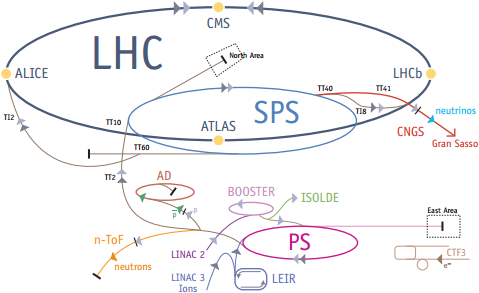
\includegraphics[width=.9\textwidth]{lhcb/lhc.png}

\column{.5\textwidth}
The main \lhc design parameters:
\resizebox{.9\textwidth}{!}{
\begin{tabular}{rr}\toprule
Circumference & 27\km\\
Center-of-mass energy & 14\tev\\
Injection energy & 450\gev\\
Field at 2 $\times$ 450\gev & 0.535\tesla\\
Field at 2 $\times$ 7\tev & 8\tesla\\
Helium temperature & 2\degk\\
Luminosity & $10^{34}\cm^{-2}s^{-1}$\\
Bunch spacing & 25\ns\\
Luminosity lifetime & 10\hr\\
Time between 2 fills & 7\hr\\
\bottomrule
\end{tabular}
}
\end{columns}
\bigskip
The \lhc operated mainly at center-of-mass energies of 7\tev and 8\tev in 2011
and 2012, respectively. In 2015, after the long  shutdown, \lhc is planned to
reach energy of 13\tev.
\end{frame}
% \begin{frame}[t]{The LHCb experiment (1)}
\small
\centering
\begin{columns}[t]
\column{.5\textwidth}
Forward spectrometer with planar detectors:
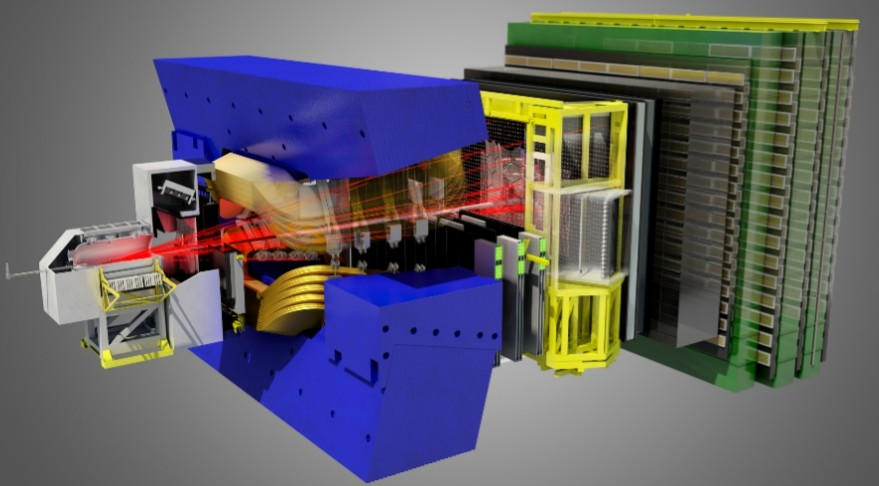
\includegraphics[width=.9\textwidth]{lhcb/lhcb-general}

\begin{itemize}
\item \textcolor{red}{LHCb uniqueness:}
\begin{itemize}
\footnotesize
\item Tracking, RICH and calorimeters cover
the full detector acceptance ($2.0< \eta <5.0$);
tracking coverage also in the backward
region ($-4.0 < \eta <-1.5$)
\item Covers just ~4\% of the solid angle but captures
~25\% of heavy quark pairs produced at the \lhc.
\item Ability to study low-pT processes at large $\eta$
\end{itemize}
\end{itemize}

\column{.5\textwidth}
Heavy quark pair production at the \lhc:
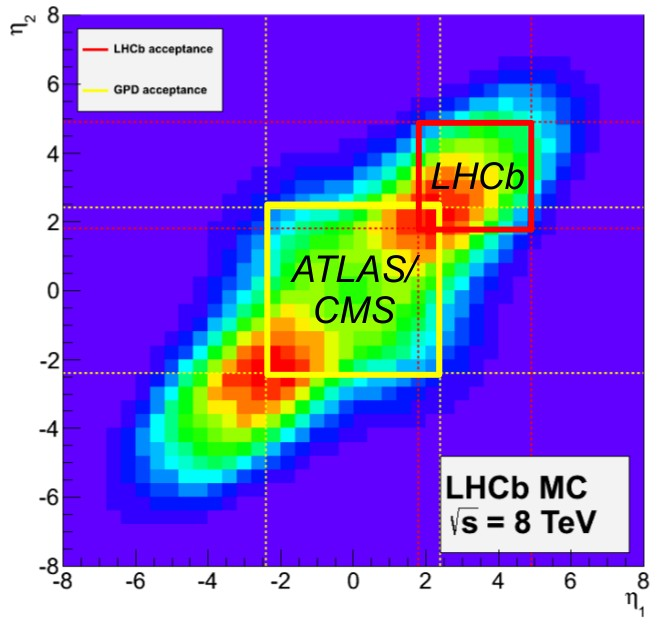
\includegraphics[width=.9\textwidth]{lhcb/bb-range}

Fraction of $b\bar{b}$ pairs in the acceptance:
\resizebox{.9\textwidth}{!}{
\begin{tabular}{rrr}\toprule
\sqs & \atlas/\cms & \lhcb\\
\midrule
7\tev & 44\% & 25\%\\
14\tev & 41\% & 24\%\\
\bottomrule
\end{tabular}
}
\end{columns}

\end{frame}
% \begin{frame}[t]{The LHCb experiment (2)}

\centering

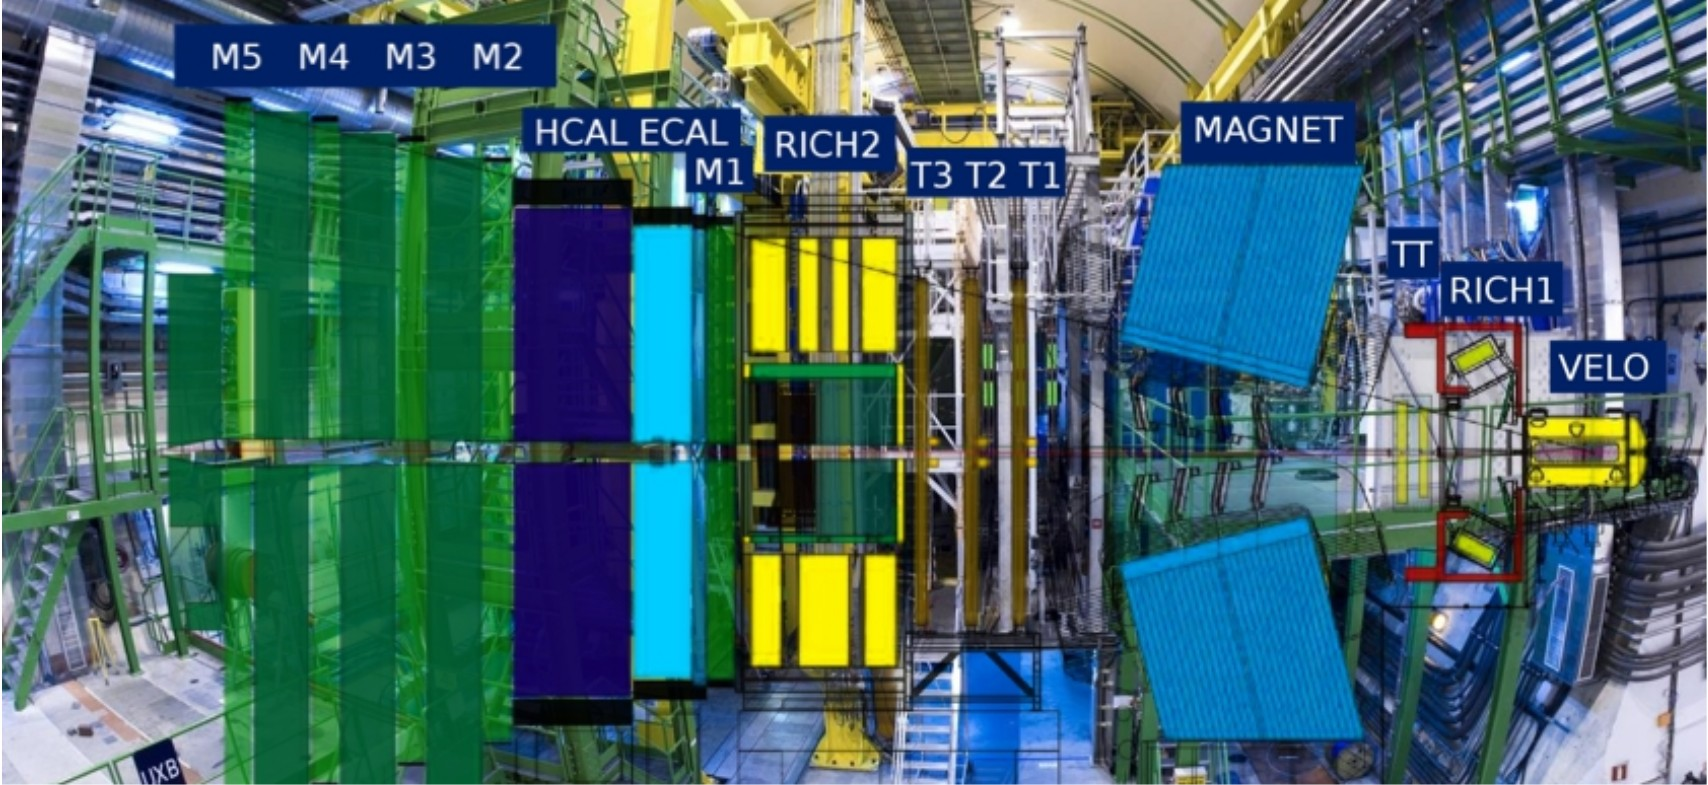
\includegraphics[width=.75\textwidth]{lhcb/lhcb-sub}

\begin{itemize}
\item Excellent tracking performance
\item High quality particle identification: robust hadron ID + photon/lepton/hadron separation
\item Selective and flexible trigger system
\end{itemize}
\end{frame}
% \begin{frame}[t]{The LHCb experiment (3)}

\begin{columns}[t]

\column{.5\textwidth}
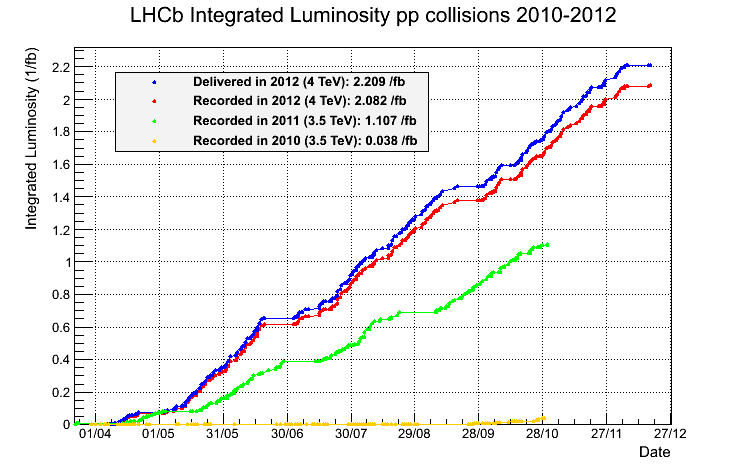
\includegraphics[width=.9\textwidth]{lhcb/lumi}

\column{.5\textwidth}
\begin{minipage}[c][.55\textheight][t]{\linewidth}
\lhcb 2010--2012 operation:

\bigskip
Integrated luminosities:

\begin{itemize}
\item $0.038\invfb$ in 2010
\item $1.107\invfb$ in 2011
\item $2.082\invfb$ in 2012
\end{itemize}

Visible  interactions:
\begin{itemize}
\item $2\times10^{14}$ visible $pp$ interactions 
\item $6\times10^{12}$ visible $c\bar{c}$ interactions 
\item $3\times10^{11}$ visible $b\bar{b}$ interactions 
\end{itemize}
\end{minipage}
\end{columns}

\begin{itemize}
\item ${\sim}93\%$ data taking efficiency
\item ${\sim}99\%$ of accumulated data are useful for physics analyses
\item Luminosity leveling: constant and moderate interaction rate throughout the data taking periods
\item Smooth data taking in 2011--2012 regardless high luminosity running 
\end{itemize}

\end{frame}
% \begin{frame}
\begin{exampleblock}{}
    \begin{center}
        {\huge Study of $\chi_{b}$ production}
    \end{center}
\end{exampleblock}
\end{frame}
\begin{frame}{Motivation}

\frametitle{Motivation}
Bound $b\bar{b}$ states, which can be produced in different spin
configurations, are an ideal laboratory for QCD tests. It's like a hydrogen
atom in QCD.
\begin{columns}[c]
\column{.4\textwidth}
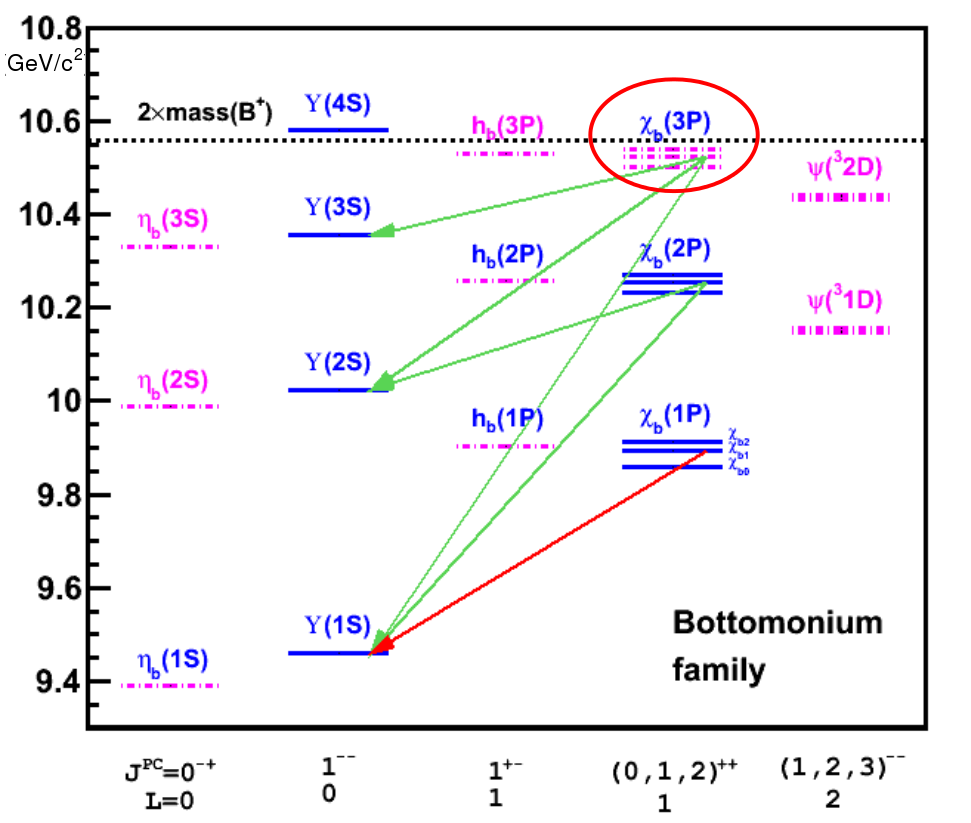
\includegraphics[width=\textwidth]{bfamily.png}
\begin{itemize}
  \item \textcolor{blue}{Measured mass}
  \item \textcolor{red}{Mass from theory}
\end{itemize}
\column{.6\textwidth}
\fontsize{9pt}{7.2}\selectfont
States with parallel quark spins (S=1):
\begin{itemize}
  \item S-wave $\Upsilon$ state.
  \item P-wave $\chi_{b}$ states, composed by 3 spin states $\chi_{b(0,1,2)}$. 
  \item $\Upsilon$ can be readily produced in the radiative decays of $\chib$.
  \item $\chi_{b}(3P)$ state recently observed by ATLAS, D0 and LHCb.
\end{itemize}
\textcolor{red}{This thesis:}
\begin{enumerate}
  \item Measurement of  $\Upsilon(NS)$ (N=1, 2, 3) fraction  originating from \chib decays as function of $p_T(\Upsilon)$.
  \item Measurement of $\chi_{b}(3P)$ mass.
\end{enumerate}
\end{columns}

\end{frame}
% \begin{frame}{Properties of quarkonium states}

{\scriptsize There is a
wide variety of quarkonium states, each differing from other by quantum
numbers: the principal quantum number ($n$), the relative angular momentum
between the quarks ($L$), the spin combination of the two quarks ($S$) and the
total angular momentum ($J$) with $J = L + S$. The spectroscopic notation
$J^{PC}$ is often used, where $P$ and $C$ are parity and
charge conjugation values, respectively. For the quarkonium states, they are
defined as $P=(-1)^{L+1}$ and $C=(-1)^{L+S}$.}

\begin{center}
\resizebox{.4\textwidth}{!}{
\begin{tabular}{lccl}\toprule
Meson & $n^{2S+1} L_J$ &  $J^{PC}$ & Mass (\mevcc)\\
\midrule
$\eta_c(1S)$    & $1^1 S_0$ & $0^{-+}$ & $2980.4 \pm 1.2$ \\
$\jpsi(1S)$    & $1^3 S_1$ & $1^{--}$ & $3096.916 \pm 0.011$ \\
$\chi_{c0}(1P)$ & $1^3 P_0$ & $0^{++}$ & $3414.75 \pm 0.31$ \\
$\chi_{c1}(1P)$ & $1^3 P_1$ & $1^{++}$ & $3510.66 \pm 0.07$ \\
$h_{c}(1P)$     & $1^3 P_1$ & $1^{++}$ & $3525.93 \pm 0.27$ \\
$\chi_{c2}(1P)$ & $1^3 P_2$ & $2^{++}$ & $3556.20 \pm 0.09$ \\
$\eta_{c}(2S)$  & $2^1 S_0$ & $0^{-+}$ & $3637 \pm 4$ \\
$\psi(2S)$      & $2^3 S_1$ & $1^{--}$ & $3686.09 \pm 0.04$ \\
\midrule
$\eta_b$        & $1^1 S_0$ & $0^{-+}$ & $9388.9 \pm 2.5 \pm 2.7$ \\
$\textcolor{red}{\Upsilon(1S)}$  & $1^3 S_1$ & $1^{--}$ & $9460.30 \pm 0.26$\\
$\textcolor{red}{\chi_{b0}(1P)}$ & $1^3 P_0$ & $0^{++}$ & $9859.44 \pm 0.42 \pm 0.31$ \\
$\textcolor{red}{\chi_{b1}(1P)}$ & $1^3 P_1$ & $1^{++}$ & $9892.78 \pm 0.26 \pm 0.31$ \\
$\textcolor{red}{\chi_{b2}(1P)}$ & $1^3 P_2$ & $2^{++}$ & $9912.21 \pm 0.26 \pm 0.31$ \\
$\textcolor{red}{\Upsilon(2S)}$  & $2^3 S_1$ & $1^{--}$ & $10023.26 \pm 0.31$ \\
$\textcolor{red}{\chi_{b0}(2P)}$ & $2^3 P_0$ & $0^{++}$ & $10232.5 \pm 0.4 \pm 0.5$ \\ 
$\textcolor{red}{\chi_{b1}(2P)}$ & $2^3 P_1$ & $1^{++}$ & $10255.46 \pm 0.22 \pm 0.5$ \\ 
$\textcolor{red}{\chi_{b2}(2P)}$ & $2^3 P_2$ & $2^{++}$ & $10268.65 \pm 0.22 \pm 0.5$ \\ 
$\textcolor{red}{\Upsilon(3S)}$  & $2^3 S_1$ & $1^{--}$ & $10355.2 \pm 0.5$ \\
\bottomrule
\end{tabular}
}
\end{center}
\end{frame}
% \begin{frame}{Theory predictions}

\footnotesize

\begin{columns}[t]
\column{.5\textwidth}
1. Prediction for the production cross sections for different radial excitations of $\chi_b$ states:

$$
\frac{\sigma^{th}[2P,1S]}{\sigma^{th}[1P,1S]} = (0.29 \pm 0.01^{th} \pm 0.1^{br}) \Bigl| \frac{R'_{2P}}{R'_{1P}}\Bigr|^2, 
$$
\begin{itemize}
\item  $\sigma^{th}[nP,mS]$ ---  sum over the possible $\chi_b(nP)$ spin
states of the production cross section for that state multiplied by its
branching fraction for the $\Upsilon(mS)$ decay.
\item $R'_{nP} \sim 1$ --- derivative of the $\chi_b(nP)$ state wave function at the origin
\end{itemize}

\textbf{Predictions for this
ratio in the range between 0.14 and 0.4 have been obtained by using different
potential models.}

\column{.5\textwidth}
2. The $\sigma(\chi_{b2})/\sigma(\chi_{b1})$ ratio prediction
\resizebox{.9\textwidth}{!}{
\setlength{\unitlength}{1mm}
\begin{picture}(75,60)
%
 \put(0,0){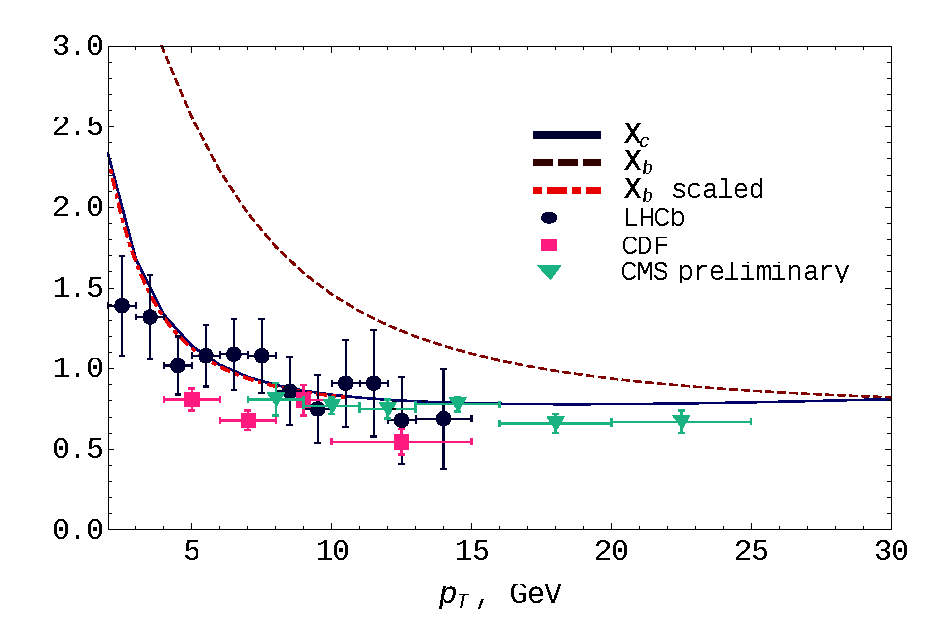
\includegraphics[width=75mm, height=60mm]{theory/ratio}}
 \put(-1,22){\begin{sideways}$\sigma({\chi_2})/\sigma({\chi_1}$)\end{sideways}}
\end{picture}
}
Transverse momentum distributions of the
$d\sigma\left[\chi_{2}\right]/d\sigma[\chi_{1}]$ ratio. Solid and dashed lines
stand for charmonium and bottomonium mesons. The dot-dashed line corresponds to
the rescaled bottomonium ratio.
\end{columns}
\end{frame}
\begin{frame}{Previous analysis at LHCb}
\begin{itemize}
\item "Measurement of the fraction of $\Upsilon(1S)$ originating from $\chi_b(1P)$ in pp collisions at \sqs=7\tev", arXiv:1209.0282, \intlum{32} \invpb
\item "Observation of the $\chi_b(3P)$ state at LHCb in pp collisions at \sqs=7\tev",
LHCb-CONF-2012-020, \intlum{0.9} \invfb.
\end{itemize}
\end{frame}
\begin{frame}
\frametitle{In this thesis}

The results in this study extend the statistical precision of 
previous LHCb measurements and add considerably more decays and higher transverse
momentum regions.  The measurement of \Y3S fraction in radiative \chibThreeP
decay was performed for the first time.
\bigskip

In each $p_T(\Upsilon)$ bin calculate:
\begin{center}
$
\frac{\sigma(pp \to \chi_b (mP) X) \times Br (\chi_b (mP) \to \Upsilon(nS) \gamma)}{\sigma(pp \to \Upsilon(nS) X)} =
\frac{N_{\chi_b (mP)\to \Upsilon(nS) \gamma}}{N_{\Upsilon(nS)}} \times \frac{\epsilon_{\Upsilon(nS)}}{\epsilon_{\chi_b (mP)\to \Upsilon(nS) \gamma}} =
\frac{N_{\chi_b (mP)\to \Upsilon(nS) \gamma}}{N_{\Upsilon(nS)}} \times \frac{1}{\epsilon^{reco}_{\gamma}}
$
\end{center}
\begin{itemize}
  \item Calculate for each $\Upsilon(nS), n=1,2,3$ and $\chi_b(mP), m=1,2,3$
  \item Get N from fits: $N_{\Upsilon}$ from  $m(\mu^+ \mu^-)$ and $N_{\chi_b \rightarrow \Upsilon \gamma}$ from [$m(\mu^+ \mu^- \gamma) - m(\mu^+ \mu^-)$] (for better resolution)
  \item Compute efficiency $\epsilon^{reco}_{\gamma}$  from Monte-Carlo simulation
\end{itemize}
\end{frame}
\begin{frame}{Analysis Plan}
\begin{enumerate}
\item Datasets
\item Determination of $\Upsilon$ yields
\item Determination of \chib yields in the following decays:
\begin{itemize}
    \item $\chi_b(1,2,3P) \to \OneS \gamma$
    \item $\chi_b(2,3P) \to \TwoS \gamma$
    \item $\chi_b(3P) \to \ThreeS \gamma$
\end{itemize}
\item Monte-Carlo efficiencies
% \item The fraction of $\Upsilon$ originating from \chib decays.
\item Systematic uncertainties 
\item Results
\end{enumerate}
\end{frame}

\begin{frame}{Datasets}
\begin{itemize}
\item Full 2011 dataset at \sqs=7\tev. \intlum{1} \invfb
\item Full 2012 dataset at \sqs=8\tev. \intlum{2} \invfb
\item Monte-Carlo simulation of \chib inclusive decays, generated
$62\times10^6$ events.
\end{itemize}
\end{frame}

\begin{frame}{The $\Upsilon$ selection}
\begin{center}
\scalebox{0.7}{
\begin{tabular}{cl}\toprule
Description & Requirement \\
\midrule
$\Upsilon$ rapidity\footnotemark &  $2.0 < y^{\Upsilon} < 4.5$ \\
Track fit quality &  $\chisq/\rm{ndf} < 4$ \\
Track $p_T$ &  $> 1$ \gevc \\
$\mumu$ vertex probability & $> 0.5 \%$ \\
Luminous region &  $|z_{PV}| < 0.5 m$ and $x_{PV}^2 + y_{PV}^2 < 100 mm^2$ \\
Kullback-Leibler distance & $> 5000$ \\
\rule{0pt}{4ex}Muon and hadron hypotheses & $\Delta\log\lum^{\mmu-\Ph} > 0$ \\
Muon probability & ProbNN  $> 0.5$ \\
\multicolumn{2}{l}{\rule{0pt}{4ex}Trigger lines:} \\
L0 &  L0DiMuon \\
HLT1 & Hlt1DiMuonHighMass \\
HLT2 & HLT2DiMuonB \\
\bottomrule
\end{tabular}
} % scale
\end{center}
\footnotetext[1]{$y = \frac{1}{2}\ln(\frac{E+p_L}{E-p_L})$, where $p_L$  is the
component of the momentum along the beam axis}
\end{frame}


\begin{frame}{The $\Upsilon$ fit model}
\setlength{\unitlength}{1mm}
\begin{columns}
\column{.5\textwidth}
\scalebox{0.7}{
  \begin{picture}(75,60)
    \put(0,0){
      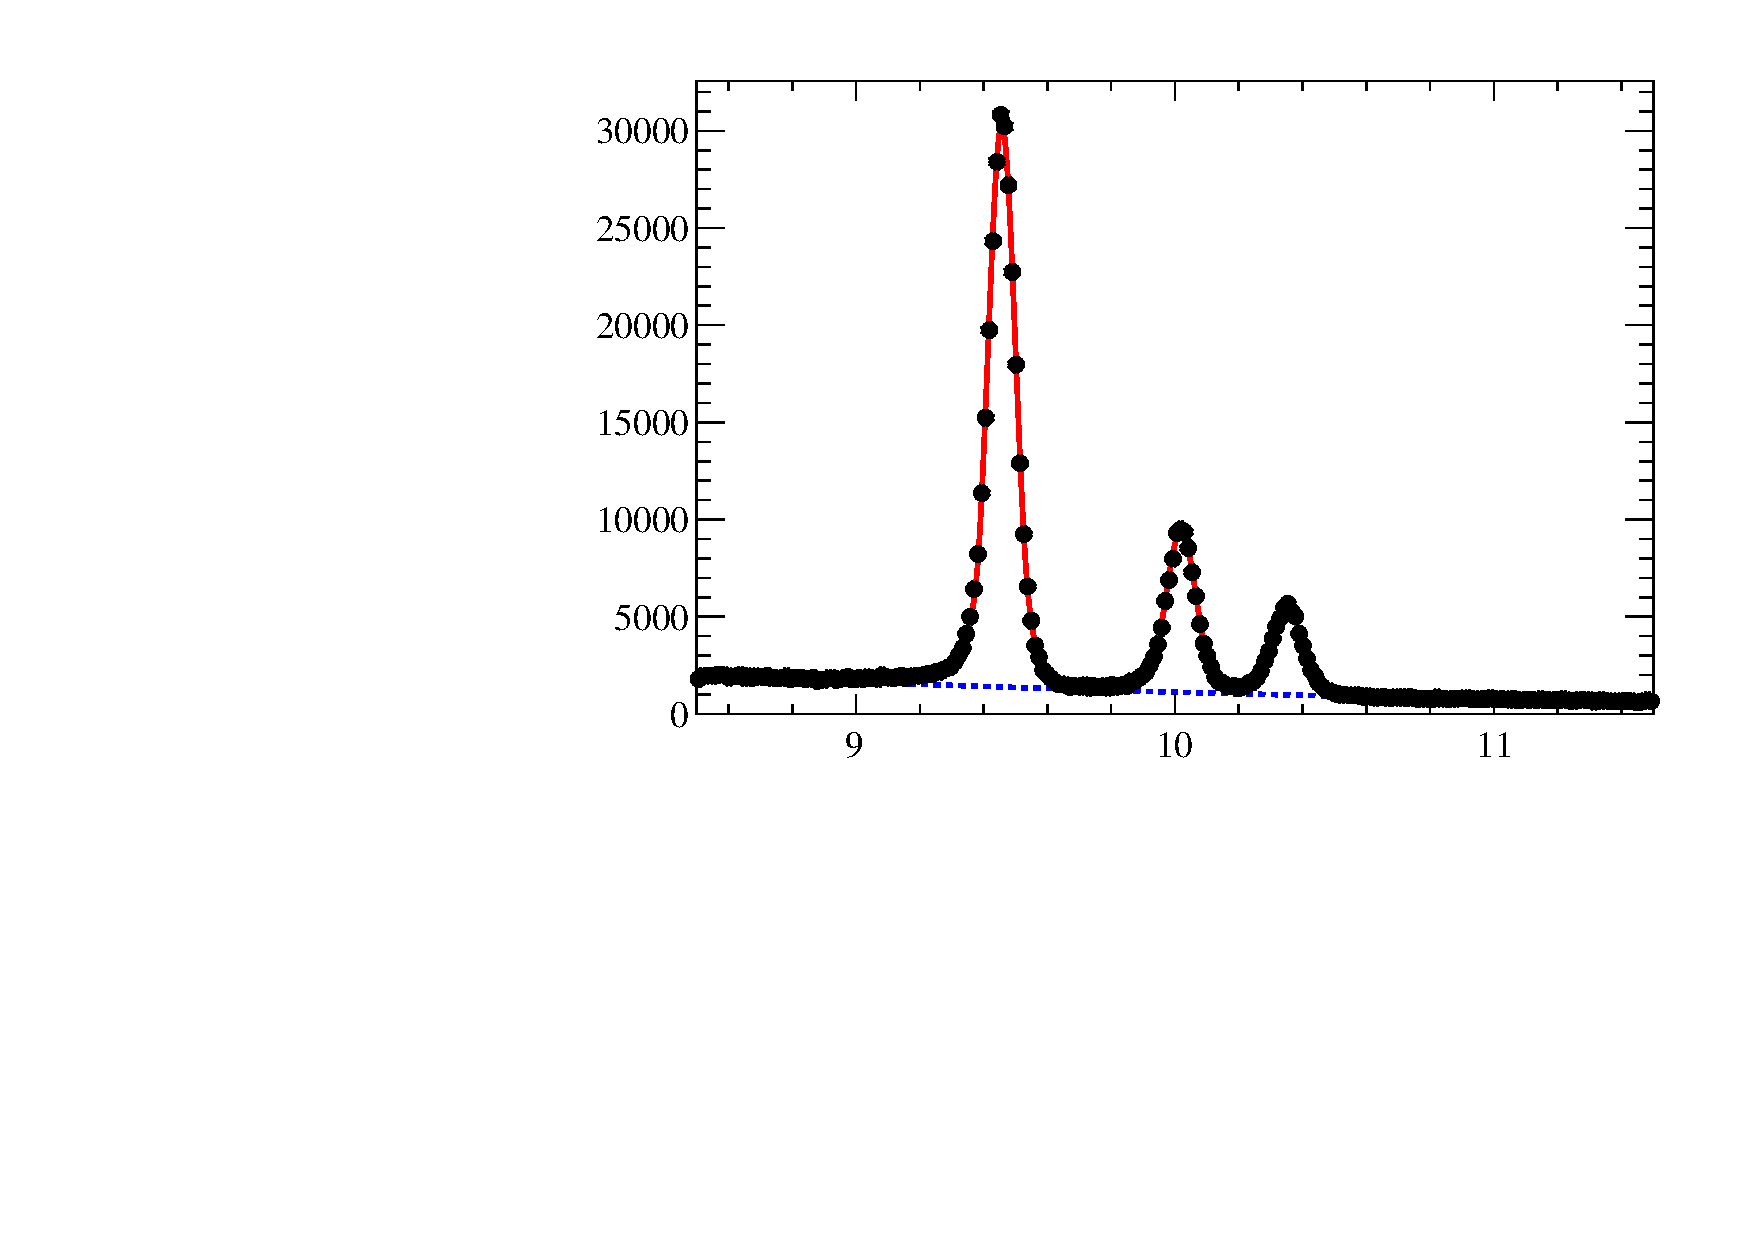
\includegraphics[width=75mm, height=60mm]{upsilon-fit/f2011_6_40}
    }
    \put(0,18){\small \begin{sideways}Candidates/(40\mevcc)\end{sideways}}
    \put(25, 0){$m_{\mumu} \left[\gevcc\right]$}
    \put(45,45){\sqs = 7 \tev}
    \put(35,38){$6 < p_T^{\mumu} < 40 \gevc$}
    
    \put(18,50){\Y1S}
    \put(40,25){\Y2S}
    \put(50,20){\Y3S}
    % \graphpaper[5](0,0)(75, 60)
  \end{picture}
}
\begin{itemize}
\item 3 Double Crystal Ball functions for signal yields. $\alpha$ and $n$ fixed
from simulation.
\item Exponential function for combinatorial background.
\end{itemize}

\column{.5\textwidth}
\resizebox{.75\textwidth}{!}{
\begin{tabular}{lrr}\toprule
 & \multicolumn{2}{c}{$\mumu$ transverse momentum intervals, \gevc}\\
 & \multicolumn{2}{c}{6 -- 40}\\
\cmidrule(r){2-3}
 & \multicolumn{1}{c}{\sqs = 7\tev} & \multicolumn{1}{c}{\sqs = 8\tev}\\
\midrule
$N_{\Y1S}$ & 283,300 $\pm$ 600 & 659,600 $\pm$ 900\\
$N_{\Y2S}$ & 87,500 $\pm$ 400 & 203,300 $\pm$ 600\\
$N_{\Y3S}$ & 50,420 $\pm$ 290 & 115,300 $\pm$ 400\\

\rule{0pt}{4ex}Background & 296,400 $\pm$ 700 & 721,300 $\pm$ 1100\\

\rule{0pt}{4ex}$\mu_{\Y1S}, \mevcc$ & 9457.02 $\pm$ 0.10 & 9455.58 $\pm$ 0.07\\
$\sigma_{\Y1S}, \mevcc$ & 42.86 $\pm$ 0.10 & 43.04 $\pm$ 0.06\\

\rule{0pt}{4ex}$\mu_{\Y2S}, \mevcc$ & 10,019.03 $\pm$ 0.21 & 10,018.05 $\pm$ 0.14\\
$\sigma_{\Y2S}, \mevcc$ & 46.38 $\pm$ 0.20 & 46.45 $\pm$ 0.14\\

\rule{0pt}{4ex}$\mu_{\Y3S}, \mevcc$ & 10,351.16 $\pm$ 0.32 & 10,349.41 $\pm$ 0.16\\
$\sigma_{\Y3S}, \mevcc$ & 48.63 $\pm$ 0.31 & 48.24 $\pm$ 0.11\\

$\tau$ & -0.3887 $\pm$ 0.0023 & -0.3819 $\pm$ 0.0015\\
\bottomrule
\end{tabular}
} % scalebox

\bigskip

\begin{itemize}
\item \Y1S mass is about 5 \mevcc lower than PDG value $9460.30 \pm  0.26$ \mevcc
% \item In this study \OneS mass was fixed to $9.456 \gevcc$ 
\end{itemize}
\end{columns}


\end{frame}


\begin{frame}{$\Upsilon$ yields as function of $p_T$}
  \setlength{\unitlength}{1mm}
  \centering
  \scalebox{0.55 }{
  \begin{picture}(150,120)
    \put(0,0){
      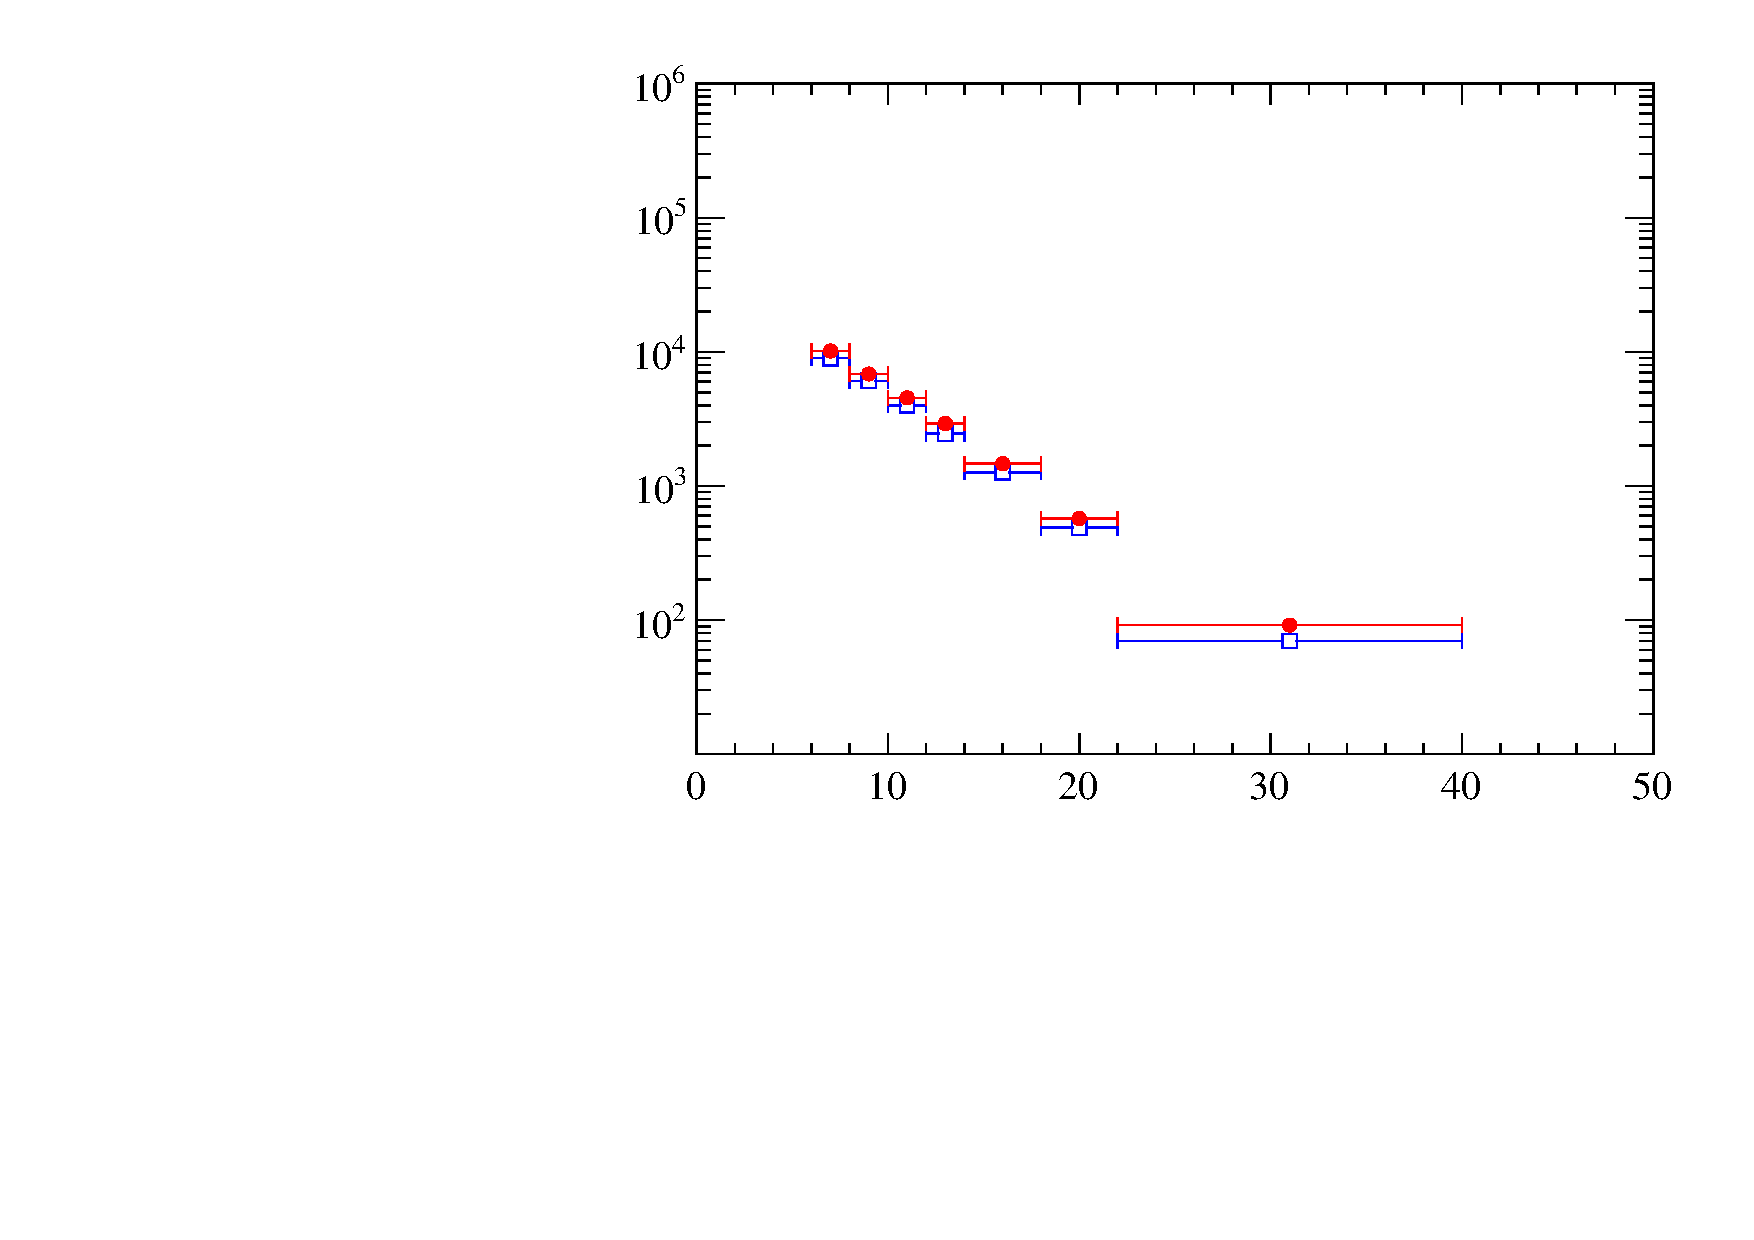
\includegraphics[width=75mm, height=60mm]{upsilon-yields/N3S_scaledbylum}
    }
    \put(0,60){
      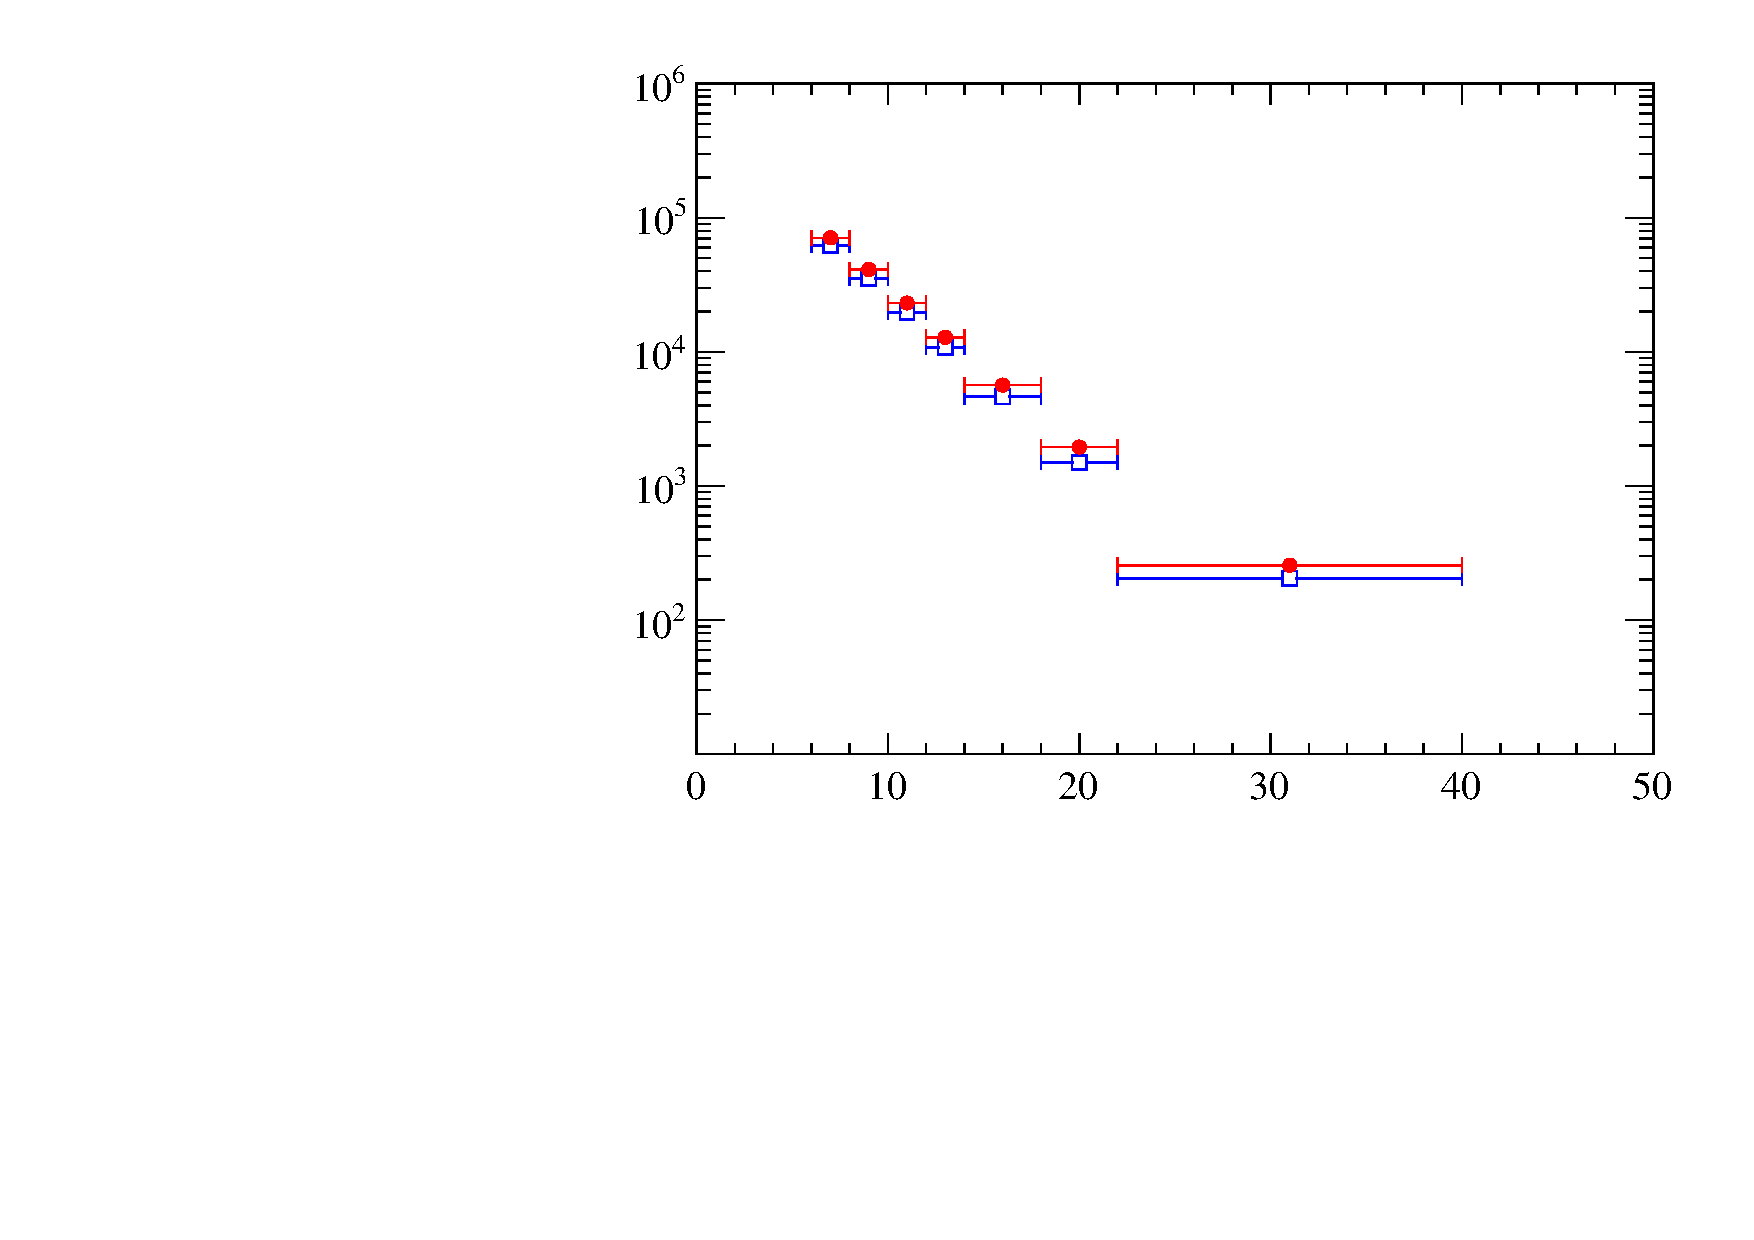
\includegraphics[width=75mm, height=60mm]{upsilon-yields/N1S_scaledbylum}
    }
    \put(75,60){
      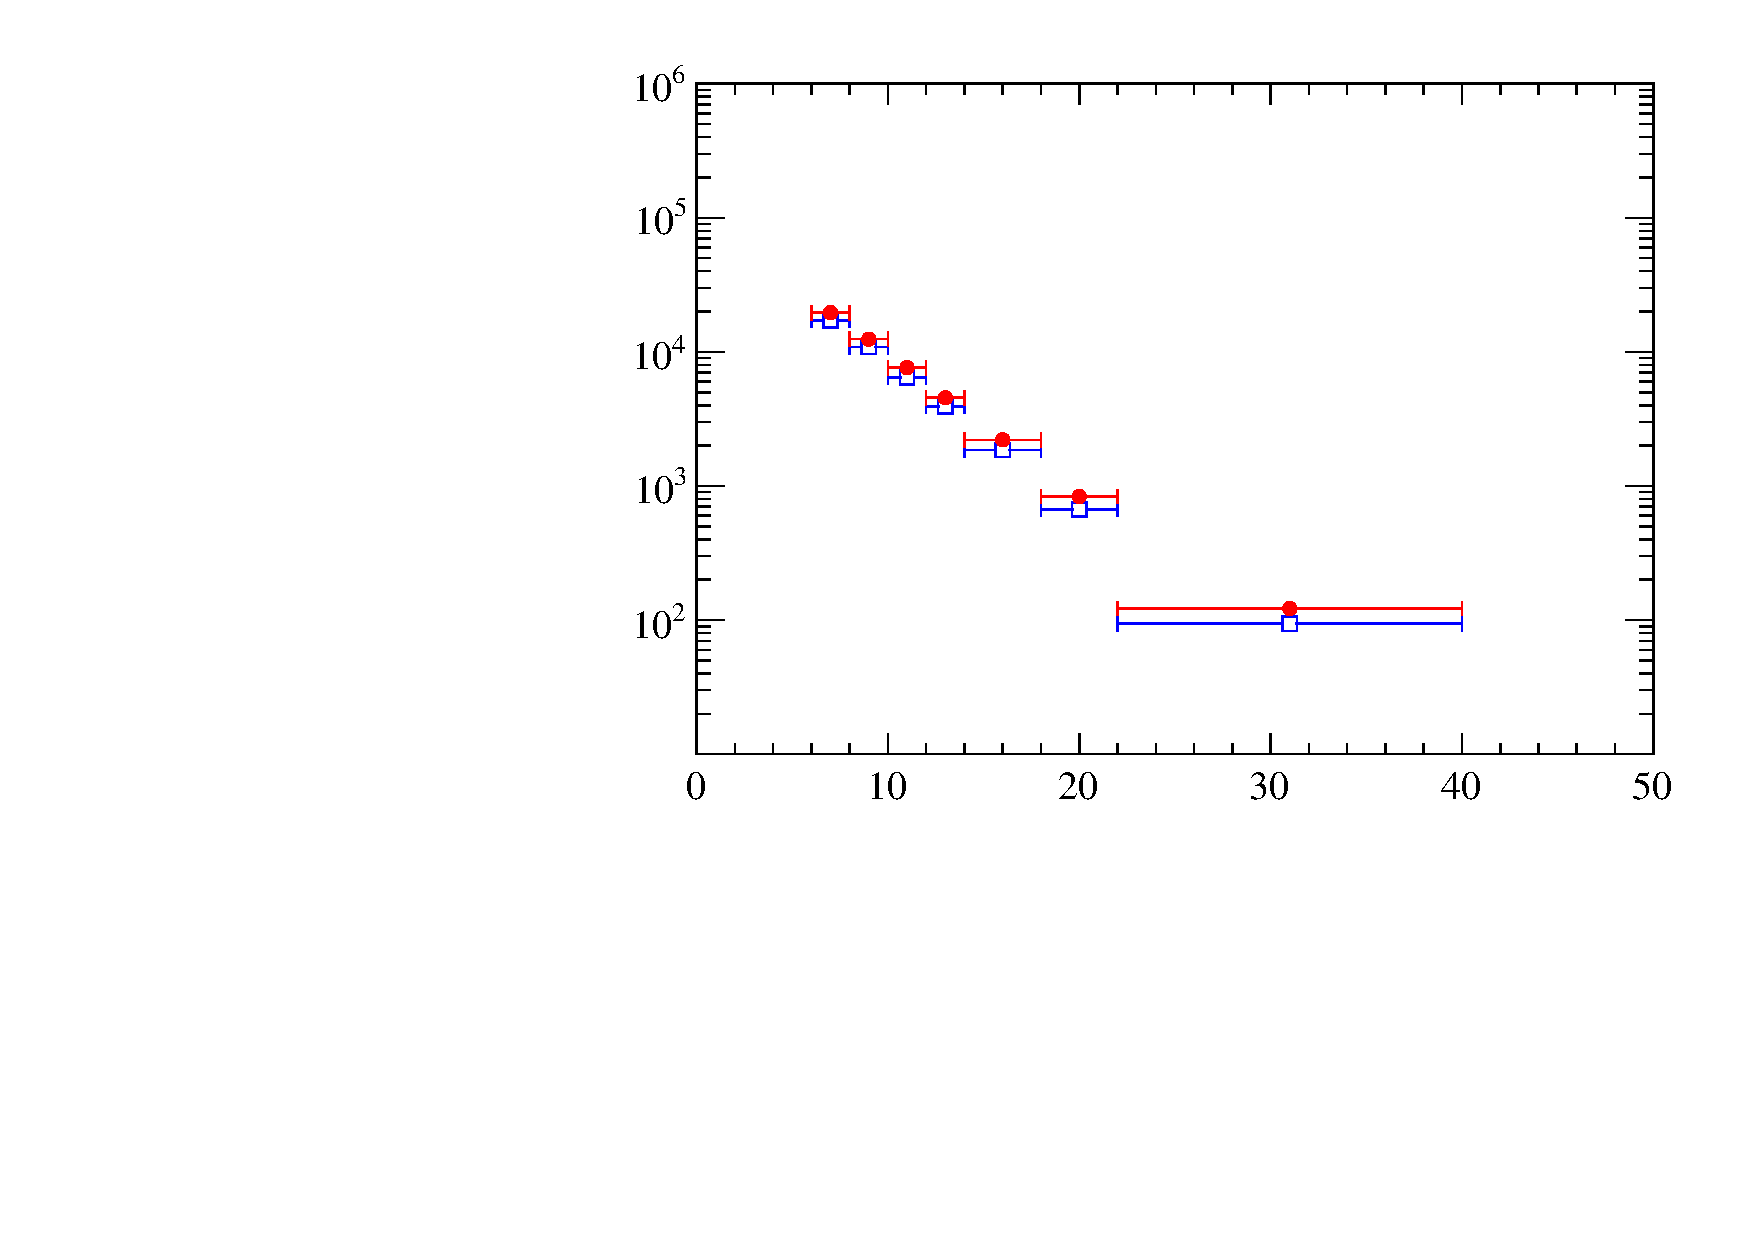
\includegraphics[width=75mm, height=60mm]{upsilon-yields/N2S_scaledbylum}
    }

    \put(2,25){\begin{sideways}Events\end{sideways}}
    \put(35,2){$p_T(\Upsilon) \left[\gevc\right]$}
    \put(55,50){$\Y3S$}

    \put(2,85){\begin{sideways}Events\end{sideways}}
    \put(35,62){$p_T(\Upsilon) \left[\gevc\right]$}
    \put(55,110){$\Y1S$}

    \put(77,85){\begin{sideways}Events\end{sideways}}
    \put(110,62){$p_T(\Upsilon) \left[\gevc\right]$}
    \put(130,110){$\Y2S$}


    \put(50,45){\textcolor{blue}{\sqs=7\tev}}
    \put(50,40){\textcolor{red}{\sqs=8\tev}}
    \put(45,45){
      
\includegraphics[width=3mm, height=2mm]{bsf}
    }
    \put(45,40){
      
\includegraphics[width=3mm, height=2mm]{rco}
    }

    \put(50,105){\textcolor{blue}{\sqs=7\tev}}
    \put(50,100){\textcolor{red}{\sqs=8\tev}}
    \put(45,105){
      
\includegraphics[width=3mm, height=2mm]{bsf}
    }
    \put(45,100){
      
\includegraphics[width=3mm, height=2mm]{rco}
    }

    \put(125,105){\textcolor{blue}{\sqs=7\tev}}
    \put(125,100){\textcolor{red}{\sqs=8\tev}}
    \put(120,105){
      
\includegraphics[width=3mm, height=2mm]{bsf}
    }
    \put(120,100){
      
\includegraphics[width=3mm, height=2mm]{rco}
    }


  % \graphpaper[5](0,0)(75, 60)
  \end{picture}
  }

Yields normalized by bin width and luminosity.

\begin{block}{}
The small difference between 7 and 8\tev data is due to the production
cross-sections, which are expected to be about 10\% larger.
\end{block}
 
\end{frame}


\begin{frame}{\chib selection}
\begin{itemize}
\item In this study photons reconstructed using the calorimeter information. 
Another approach uses photon conversions in $e^{+}e^{-}$ pairs  --- this method
has better invariant mass resolution, but requires more statistics.

\item Cuts on $\gamma$:
\begin{center}
\scalebox{0.9}{
\begin{tabular}{lr}\toprule
Transverse momentum of $\gamma$ & $p_T(\gamma) > 600 \mevc$ \\
Polar angle of $\gamma$ in the $\mumu\gamma$ rest frame & $\cos\theta_{\gamma} > 0$ \\
Confidence level of $\gamma$ & $cl(\gamma) > 0.01$ \\
\bottomrule
\end{tabular}
}
\end{center}

\bigskip

\item Dimuon mass windows:
\begin{center}
\scalebox{0.6}{
\begin{tabular}{lrr}\toprule
\multicolumn{1}{c}{Decay} & \multicolumn{1}{c}{Cut} & \multicolumn{1}{c}{Description}\\
\midrule
$\chib(1,2,3P) \to \Upsilon(1S)$ & $9310 < \mumu < 9600 \mevc$ & $3 \sigma_{\Y1S} < \mumu < 2.5 \sigma_{\Y1S} \mevc$\\
$\chib(2,3P) \to \Upsilon(2S)$ & $9870 < \mumu < 10090  \mevc$ &  $3 \sigma_{\Y2S} < \mumu < \sigma_{\Y2S} \mevc$\\
$\chib(3P) \to \Upsilon(3S)$ & $10300 < \mumu < 10526  \mevc$ &   $\sigma_{\Y3S} < \mumu < 3 \sigma_{\Y3S} \mevc$\\
\bottomrule
\end{tabular}
}
\end{center}

\end{itemize}
\end{frame}

\begin{frame}{$\chi_{b1,2}(1,2,3P) \to \OneS \gamma$ fit model}
\begin{columns}
\column{.5\textwidth}
  \centering
  \setlength{\unitlength}{1mm}
  \begin{picture}(50,80)
      %
    \put(0,0){
      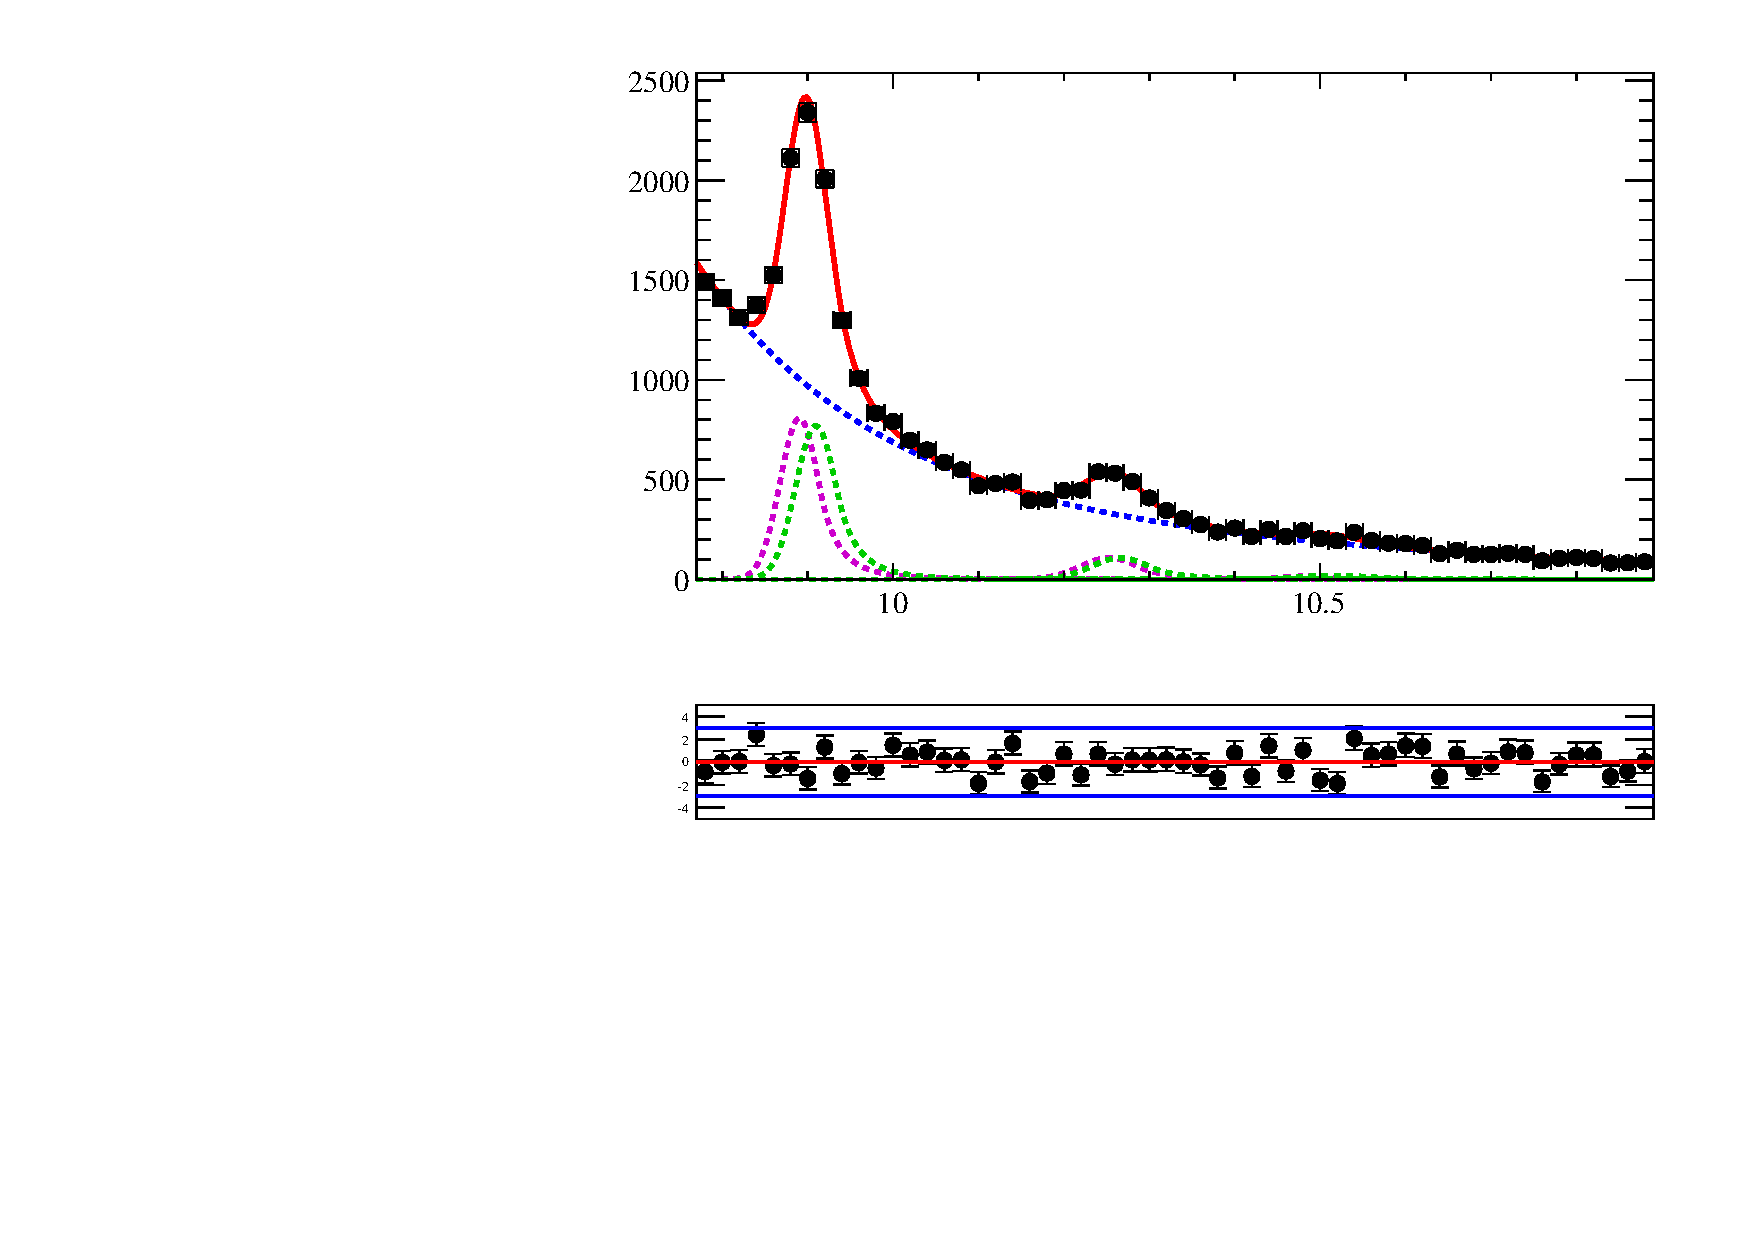
\includegraphics[width=50mm, height=40mm]{chib1s-fit/f2012_14_40}
    }
    
    \put(0,40){
      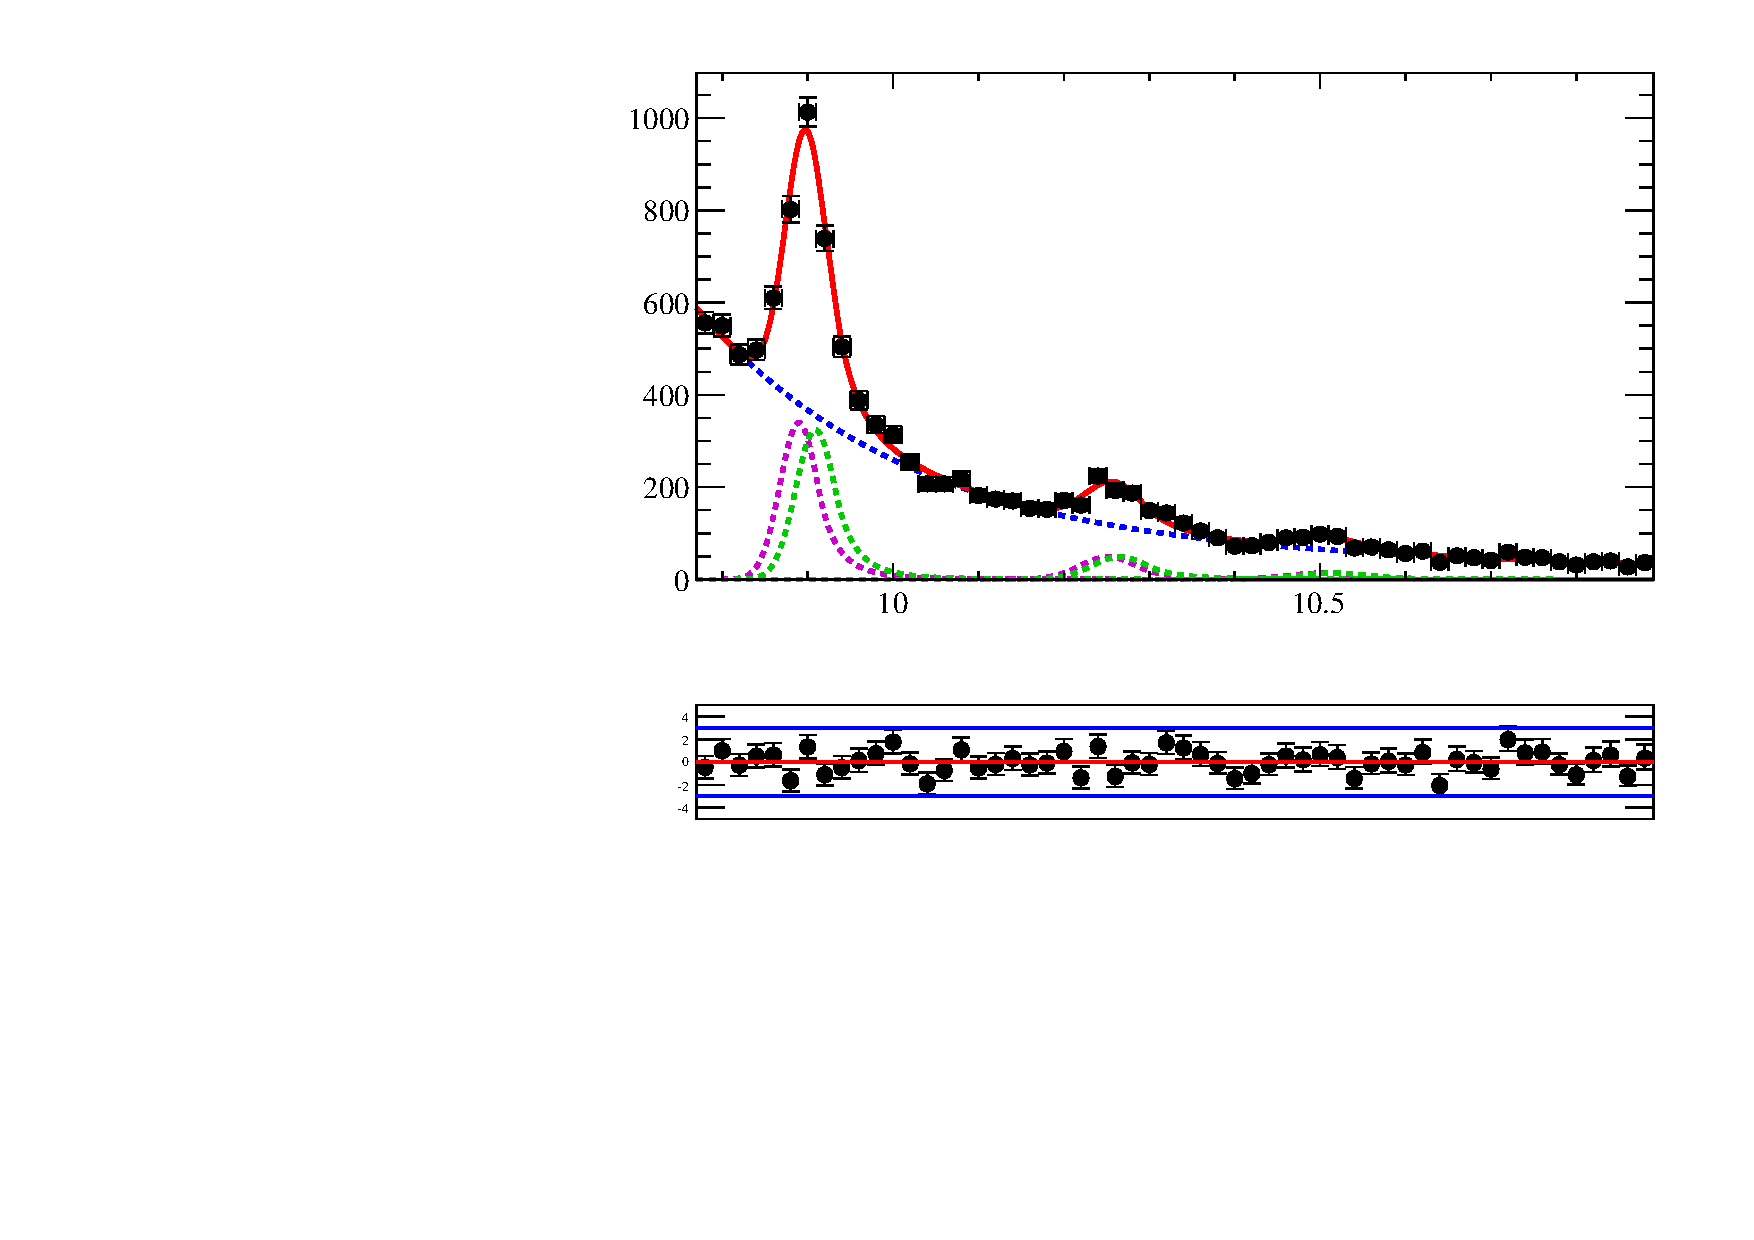
\includegraphics[width=50mm, height=40mm]{chib1s-fit/f2011_14_40}
    }

    \put(0,15){\tiny \begin{sideways}Candidates/(20\mevcc)\end{sideways}}
    \put(5,9){\tiny $m_{\mumu \gamma} - m_{\mumu} + m_{\Y1S}^{PDG} \left[\gevcc\right]$}
    \put(25,30){$\sqrt{s} = 8\tev$}
    \put(16,25){\tiny $14 < p_T^{\Y1S} < 40 \gevc$}
    
    \put(0,55){\tiny \begin{sideways}Candidates/(20\mevcc)\end{sideways}}
    \put(5, 49){\tiny $m_{\mumu \gamma} - m_{\mumu} + m_{\Y1S}^{PDG} \left[\gevcc\right]$}
    \put(25,70){$\sqrt{s} = 7\tev$}
    \put(16,65){\tiny $14 < p_T^{\Y1S} < 40 \gevc$}
    
    \put(15,75){\tiny \chibOneP}
    \put(25,60){\tiny \chibTwoP}
    \put(35,57){\tiny \chibThreeP}
    \put(15,35){\tiny \chibOneP}
    \put(25,20){\tiny \chibTwoP}
    \put(35,17){\tiny \chibThreeP}
        

    % \graphpaper[5](0,0)(50, 80)        
  \end{picture}
\column{.5\textwidth}
\begin{itemize}
\item One Crystal Ball (CB) for each $\chi_{b1,2}(1P,2P,3P)$ state: 6 CB in total
\item Exclude the study of $\chi_{b0}$ due to its low radiative branching ratio.
\item Product of exponential and linear combination of 
polynomials  for combinatorial background.
\end{itemize}
\end{columns}
\end{frame}

\begin{frame}{$\chi_{b1,2}(1,2,3P) \to \OneS \gamma$ fit model (2)}
\begin{columns}[T]
\column{.6\textwidth}
\begin{itemize}
\item Free parameters: $\mu_{\chi_{b1}(1P)}$, yields and background parameters.
\item Linked parameters for \chibone and \chibtwo signals:
    \begin{itemize}
    \item $\mu_{\chi_{b2}(jP)} = \mu_{\chi_{b1}(jP)} + \Delta m_{\chi_{b2}(jP)}^{PDG}$, j=1,2
    \item $\mu_{\chi_{b2}(3P)} = \mu_{\chi_{b1}(3P)} + \Delta m_{\chi_{b2}(3P)}^{theory}$
    \item $N_{\chi_{b}} = \lambda N_{\chi_{b1}} + (1-\lambda) N_{\chi_{b2}}$
    \item $\sigma_{\chi_{b2}} = \sigma_{\chi_{b1}}$
    \end{itemize}
\item Other linked parameters:    
    \begin{itemize}
        \item $\mu_{\chiboneTwoP} = \mu_{\chiboneOneP} + \Delta m_{\chi_{b1}(2P)}^{PDG}$
        \item $\mu_{\chiboneThreeP} = \mu_{\chiboneOneP} + \Delta m_{\chi_{b1}(3P)}$ ($\Delta m_{\chi_{b1}(3P)}$ measured in this study)
    \end{itemize}
\item Fixed parameters from MC study:
    \begin{itemize}
    \item $\sigma_{\chiboneOneP}$ \scriptsize{scaled by 1.17}, $\frac{\sigma_{\chiboneTwoP}}{\sigma_{\chiboneOneP}}$,$\frac{\sigma_{\chiboneThreeP}}{\sigma_{\chiboneOneP}}$
    \item $\alpha$ and $n$ parameters of CB.
    \end{itemize}
\end{itemize}
\column{.4\textwidth}
\resizebox{.9\textwidth}{!}{
\begin{tabular}{lrr}\toprule
 & \multicolumn{2}{c}{$\Upsilon(1S)$ transverse momentum intervals, \gevc}\\
 & \multicolumn{2}{c}{14 -- 40}\\
\cmidrule(r){2-3}
 & \multicolumn{1}{c}{\sqs = 7\tev} & \multicolumn{1}{c}{\sqs = 8\tev}\\
\midrule
$N_{\chibOneP}$ & 2090 $\pm$ 80 & 5070 $\pm$ 130\\
$N_{\chibTwoP}$ & 450 $\pm$ 50 & 1010 $\pm$ 80\\
$N_{\chibThreeP}$ & 150 $\pm$ 40 & 220 $\pm$ 60\\

\rule{0pt}{4ex}Background & 8830 $\pm$ 130 & 23,910 $\pm$ 210\\

\rule{0pt}{4ex}$\mu_{\chiboneOneP}, \mevcc$ & 9889.7 $\pm$ 1.0 & 9890.3 $\pm$ 0.7\\
$\sigma_{\chiboneOneP}, \mevcc$ & 22.0 & 22.5\\
$\sigma_{\chi_{b1}(2P)} / \sigma_{\chi_{b1}(1P)}$ & 1.5 & 1.5\\
$\sigma_{\chi_{b1}(3P)} / \sigma_{\chi_{b1}(1P)}$ & 1.86 & 1.86\\

\rule{0pt}{4ex}$\tau$ & -2.6 $\pm$ 0.5 & -3.27 $\pm$ 0.30\\
$c_0$ & -0.08 $\pm$ 0.12 & 0.07 $\pm$ 0.06\\
$c_1$ & 1.33 $\pm$ 0.04 & 0.29 $\pm$ 0.04\\

\rule{0pt}{4ex}$\chi^2 / n.d.f$ & 1.03 & 1.24\\
\bottomrule
\end{tabular}
} % scalebox

\bigskip

{\tiny \textcolor{blue}{ $\chi_{b1}(1P)$ mass agrees with the PDG value
$9892.78 \pm 0.26\stat \pm0.31\syst \mevcc$.}}
\end{columns}


\end{frame}

\begin{frame}{Mass of \chiboneOneP in $\chib \to \OneS \gamma$ decay}
\begin{center}
\resizebox{.5\textwidth}{!}{
\setlength{\unitlength}{1mm}
\begin{picture}(70,50)
  %
\put(0,0){
  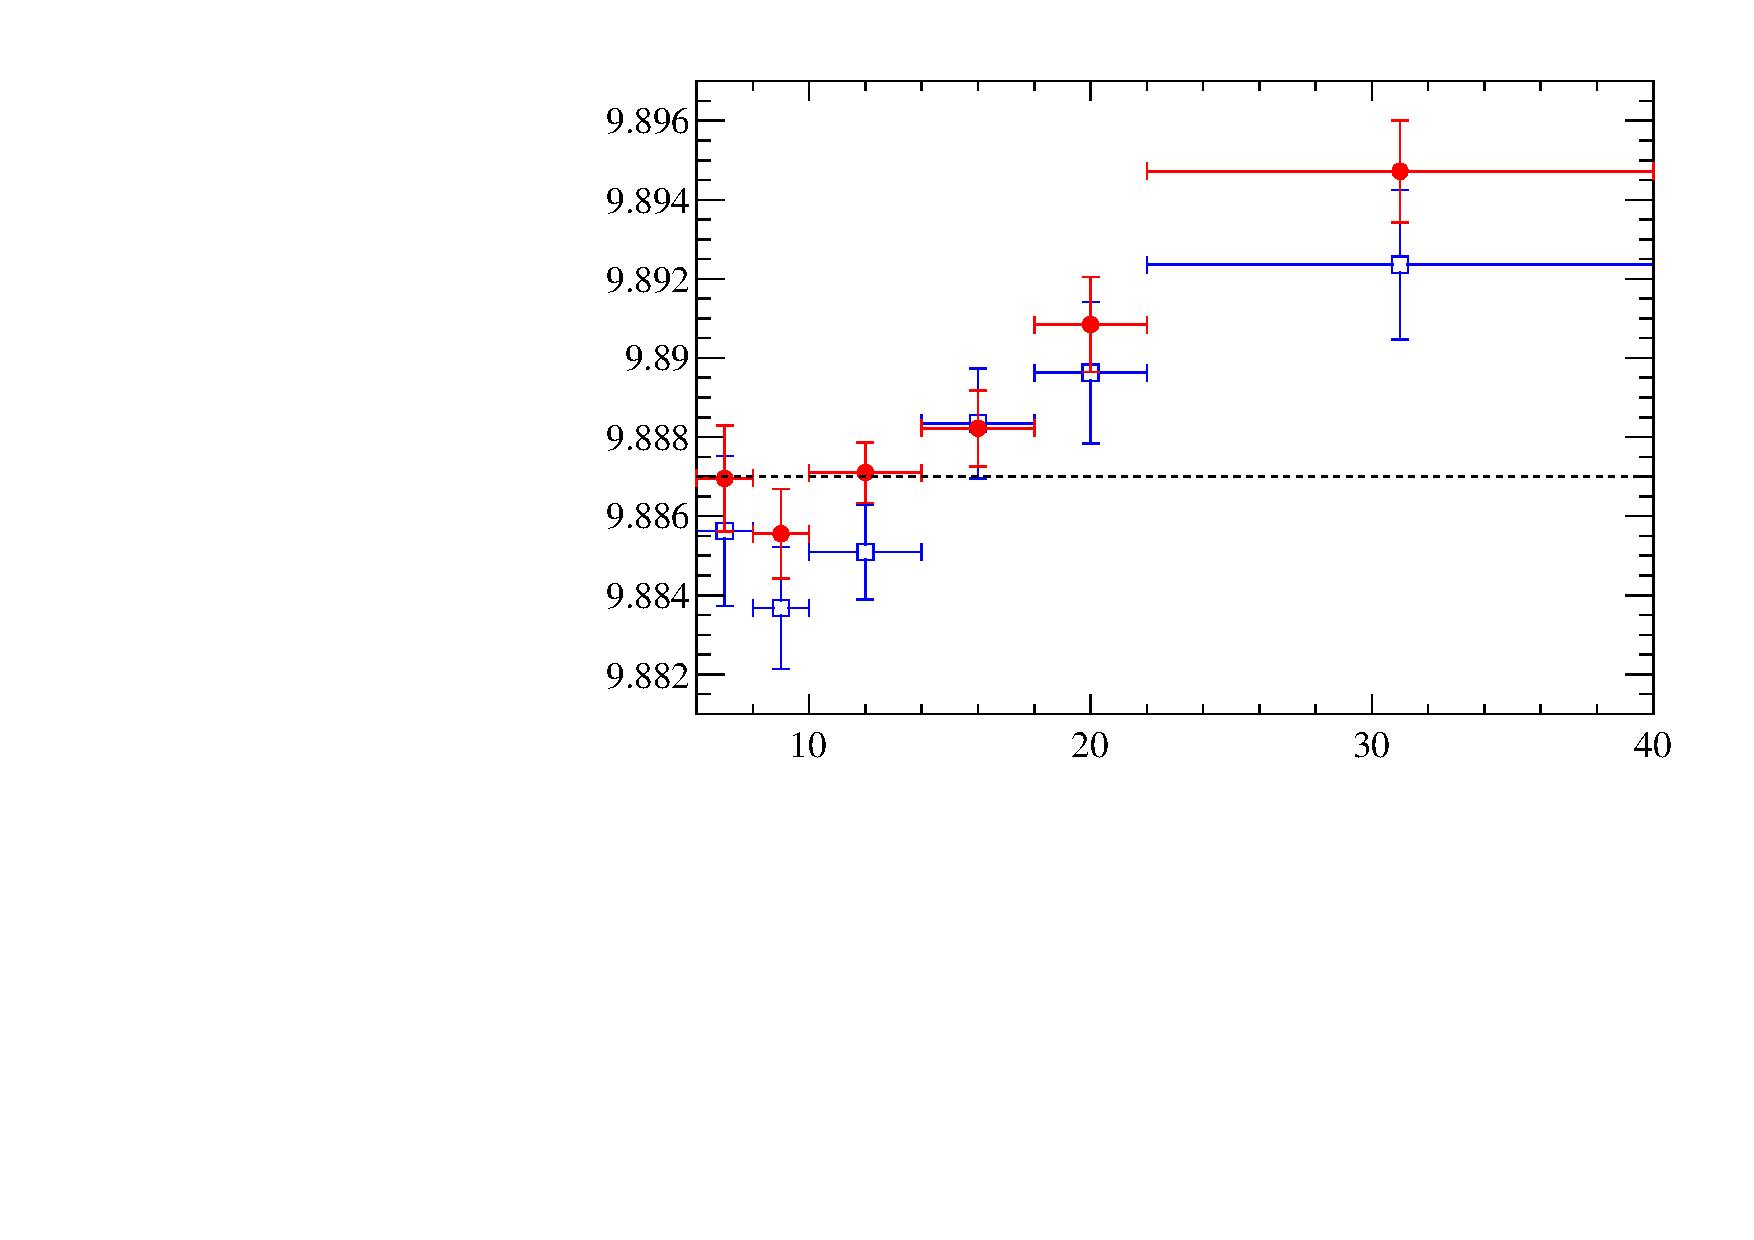
\includegraphics[width=70mm, height=50mm]{chib1s-m/mass1p}
}

\put(27, 15){\textcolor{blue}{\sqs=7\tev}, \textcolor{red}{\sqs=8\tev}}
% \put(27, 40){\textcolor{blue}{\sqs=7\tev}, \textcolor{red}{\sqs=8\tev}}
\put(0,12){\begin{sideways}\chiboneOneP mass \gevcc\end{sideways}}
\put(20,1){$p_T^{\Y1S} \left[\gevc\right]$}
\end{picture}
}
\end{center}
\begin{alertblock}{}
The major cause of  \chiboneOneP mass floating in 10 \mevcc range can be the unknown fraction
between $N_{\chibone}$ and $N_{\chibtwo}$ yields ($\lambda$ parameter). 
We have only theoretical prediction for $\lambda$ value . In this study
$\lambda$ is fixed to 0.5 for all $\chib$ decays.
\end{alertblock}

In the following, this mass was fixed to $9.887\gevcc$  which is the value
measured on the combined 2011 and 2012 datasets. A systematic uncertainty due
to this assumption has been assigned.

\end{frame}
\begin{frame}{$\chi_b$ yields in $\chi_b \to \OneS \gamma$ decays}
  \setlength{\unitlength}{1mm}
  \centering
  \resizebox{0.65\textwidth}{!}{
  \begin{picture}(150,120)
    \put(0,0){
      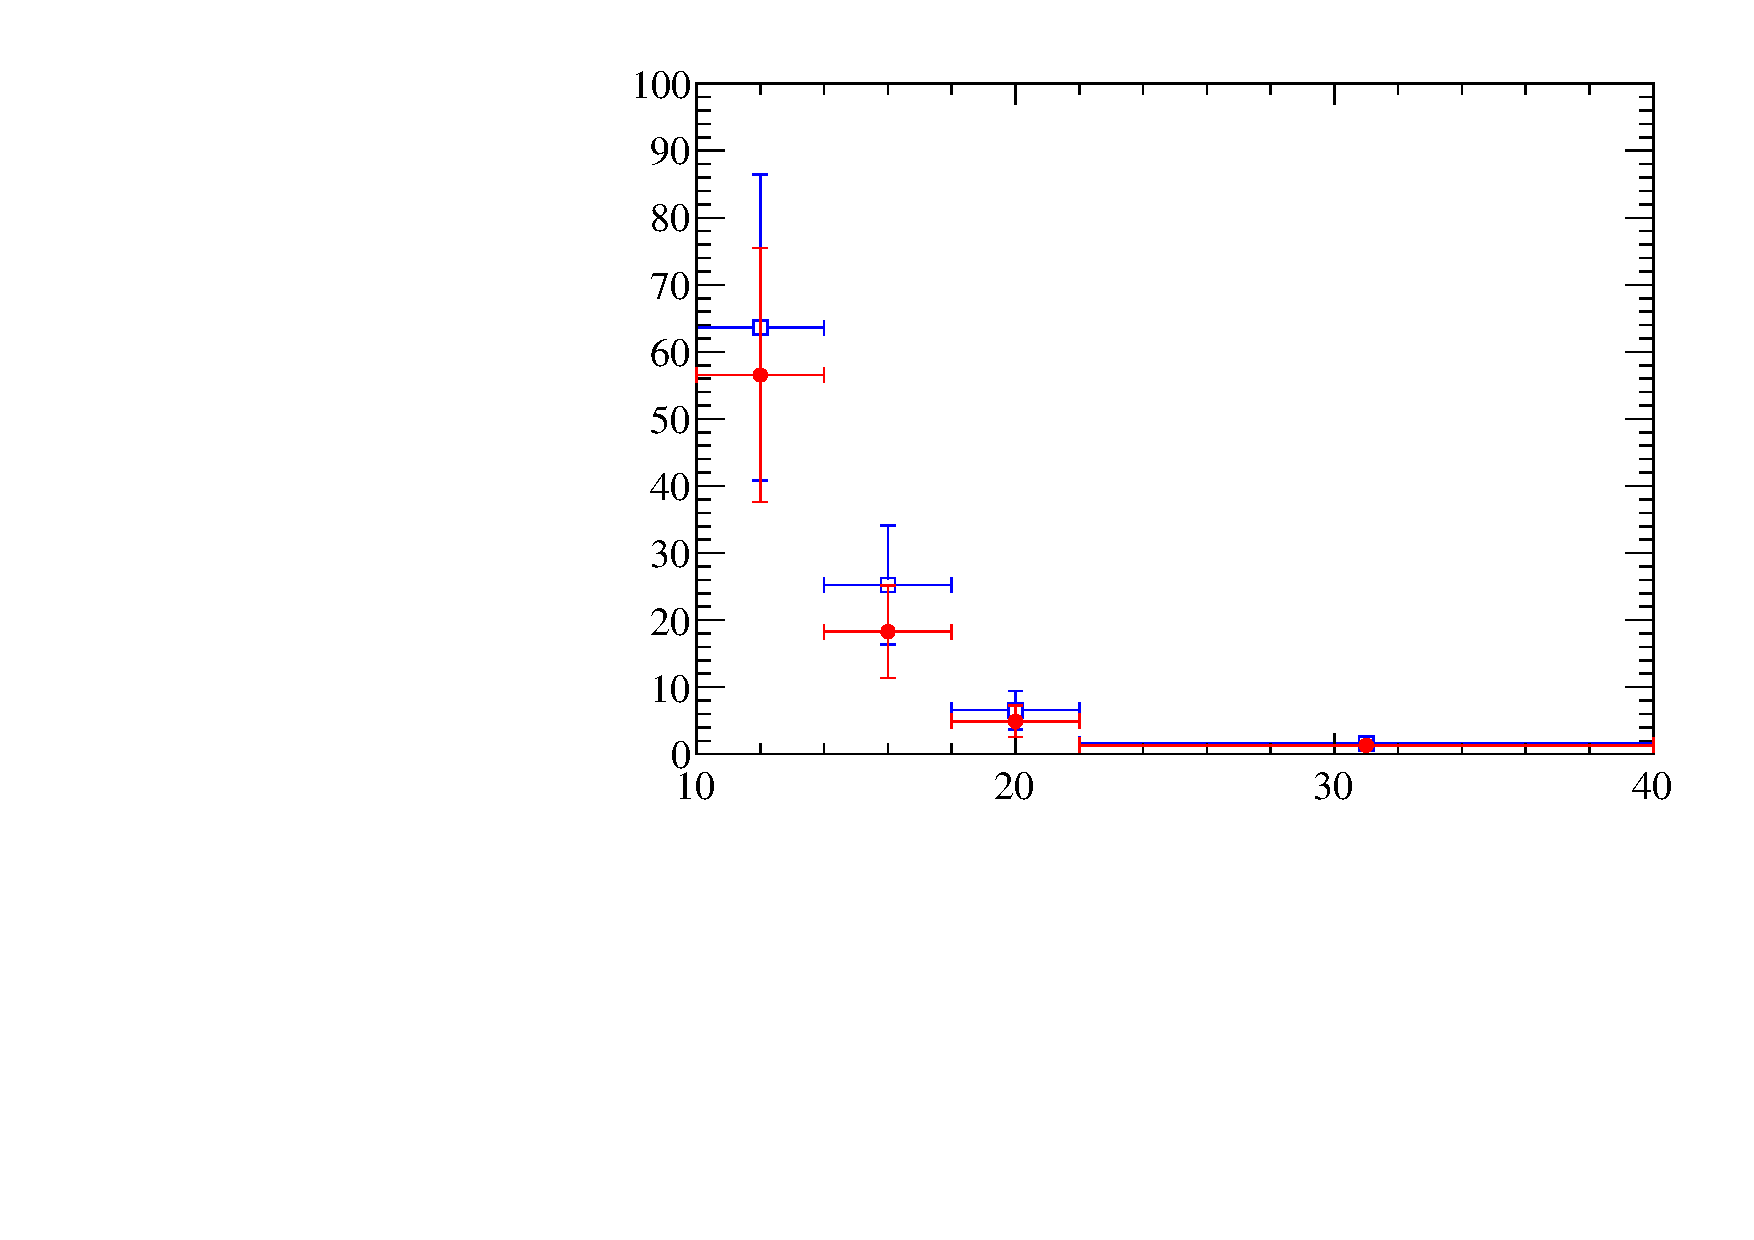
\includegraphics[width=75mm, height=60mm]{chib1s-yields/N3P_scaledbylum}
    }
    \put(0,60){
      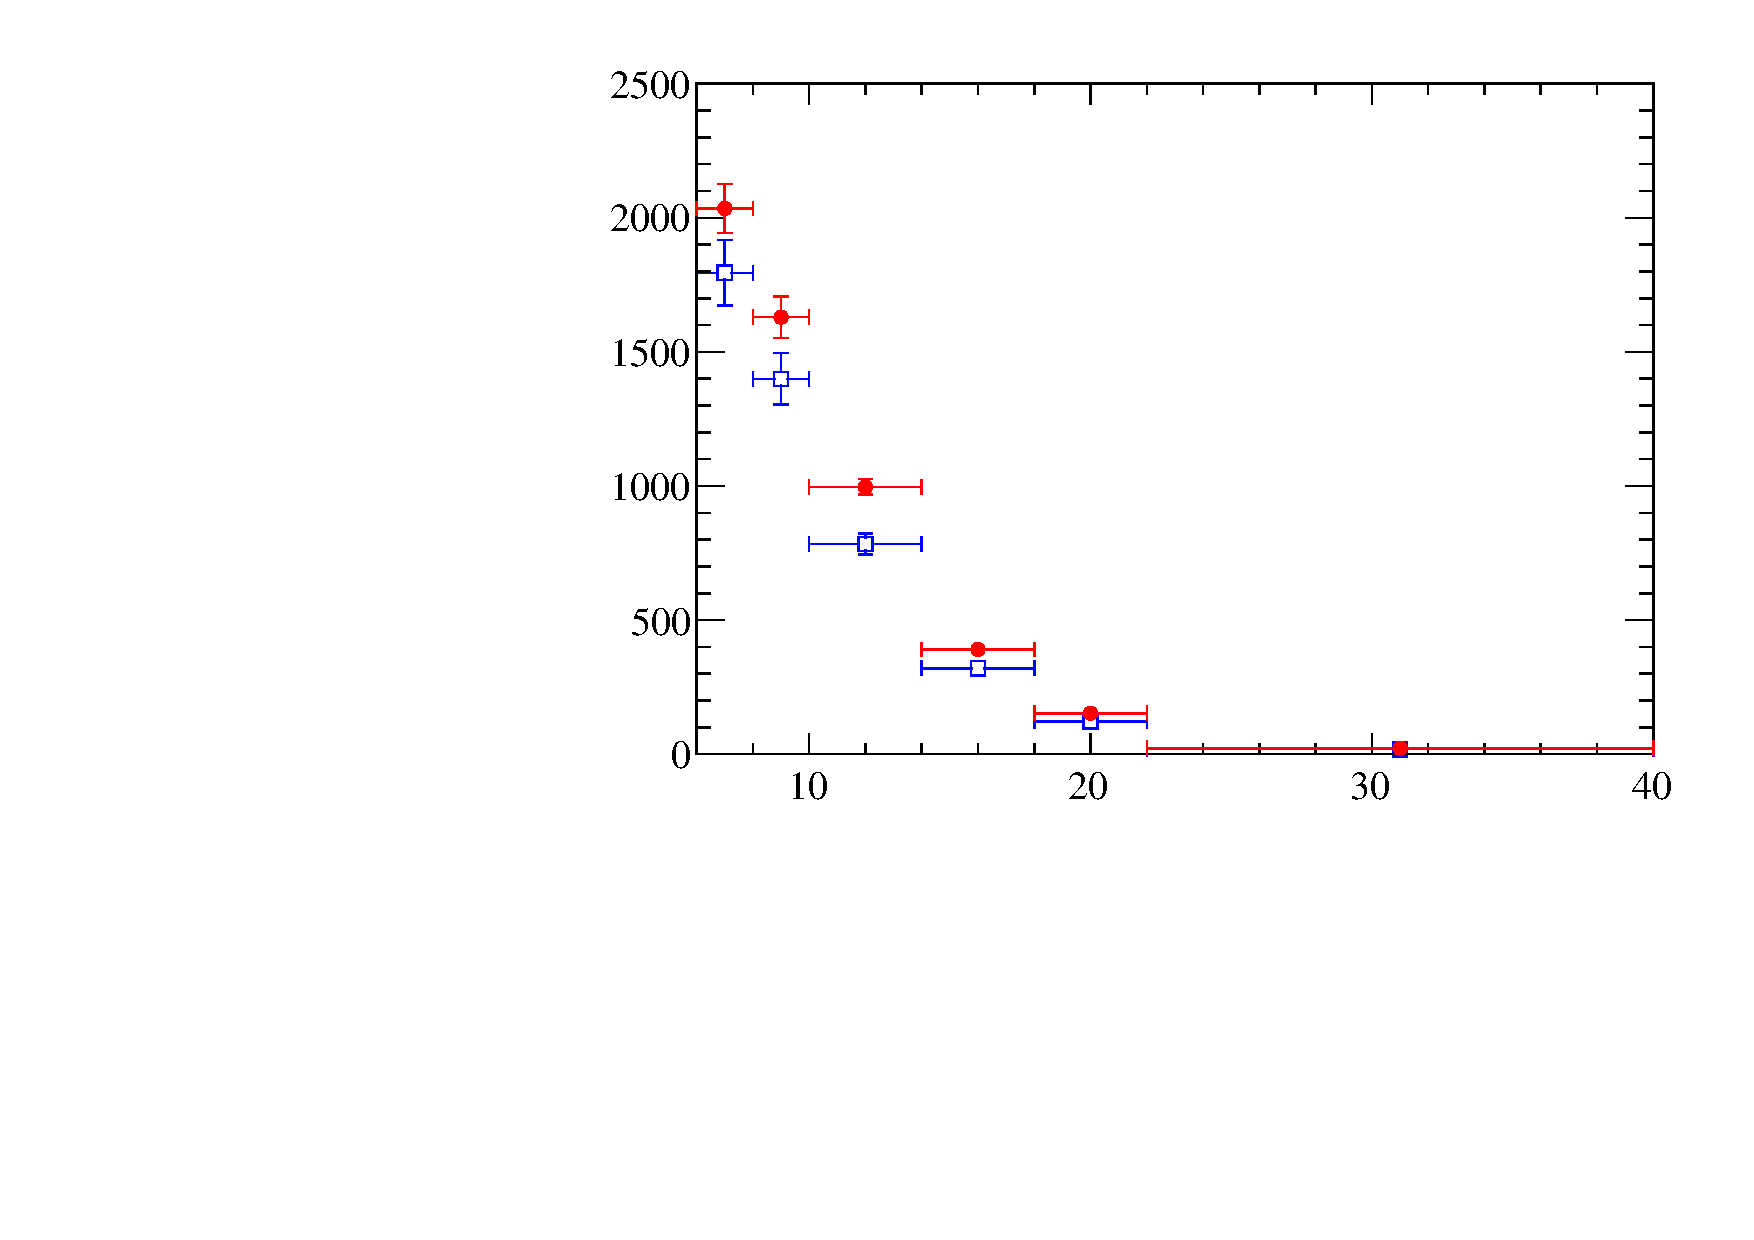
\includegraphics[width=75mm, height=60mm]{chib1s-yields/N1P_scaledbylum}
    }
    \put(75,60){
      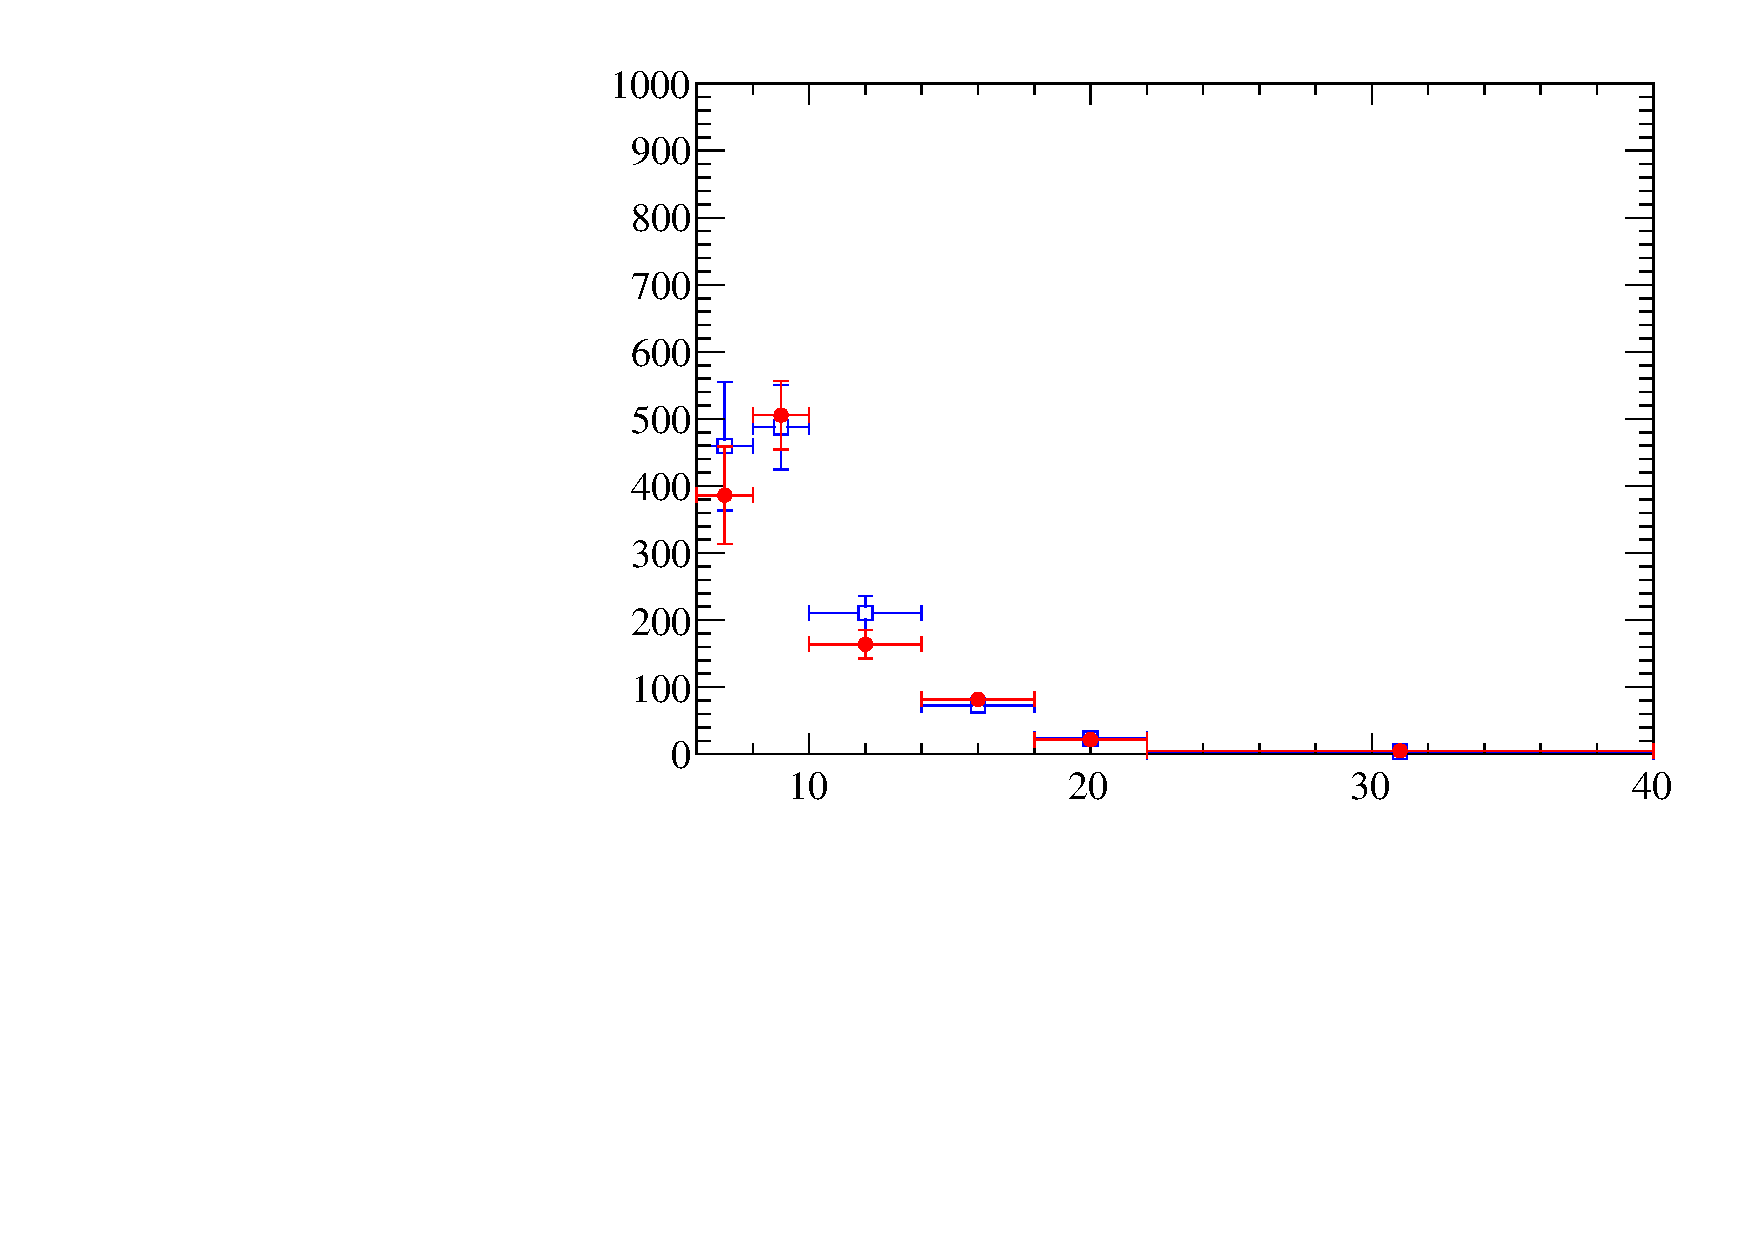
\includegraphics[width=75mm, height=60mm]{chib1s-yields/N2P_scaledbylum}
    }

    \put(2,25){\begin{sideways}Events\end{sideways}}
    \put(35,2){$p_T^{\Y1S} \left[\gevc\right]$}
    \put(55,50){$\chibThreeP$}

    \put(2,85){\begin{sideways}Events\end{sideways}}
    \put(35,62){$p_T^{\Y1S} \left[\gevc\right]$}
    \put(55,110){$\chibOneP$}

    \put(77,85){\begin{sideways}Events\end{sideways}}
    \put(110,62){$p_T^{\Y1S} \left[\gevc\right]$}
    \put(130,110){$\chibTwoP$}


    \put(50,45){\textcolor{blue}{\sqs=7\tev}}
    \put(50,40){\textcolor{red}{\sqs=8\tev}}
    \put(45,45){
      
\includegraphics[width=3mm, height=2mm]{bsf}
    }
    \put(45,40){
      
\includegraphics[width=3mm, height=2mm]{rco}
    }

    \put(50,105){\textcolor{blue}{\sqs=7\tev}}
    \put(50,100){\textcolor{red}{\sqs=8\tev}}
    \put(45,105){
      
\includegraphics[width=3mm, height=2mm]{bsf}
    }
    \put(45,100){
      
\includegraphics[width=3mm, height=2mm]{rco}
    }

    \put(125,105){\textcolor{blue}{\sqs=7\tev}}
    \put(125,100){\textcolor{red}{\sqs=8\tev}}
    \put(120,105){
      
\includegraphics[width=3mm, height=2mm]{bsf}
    }
    \put(120,100){
      
\includegraphics[width=3mm, height=2mm]{rco}
   }
  % \graphpaper[5](0,0)(75, 60)
  \end{picture}
}  
\begin{center}
Yields normalized by bin width and luminosity.
\end{center}  
\begin{block}{}
The small difference between 7 and 8\tev data is due to the production
cross-sections, which are expected to be about 10\% larger..
\end{block}
\end{frame}


\begin{frame}{$\chi_{b1,2}(2,3P) \to \TwoS \gamma$ fit model}
\begin{columns}[T]
\column{.5\textwidth}
  \centering
  \setlength{\unitlength}{1mm}
  \begin{picture}(50,80)
      %
    \put(0,0){
      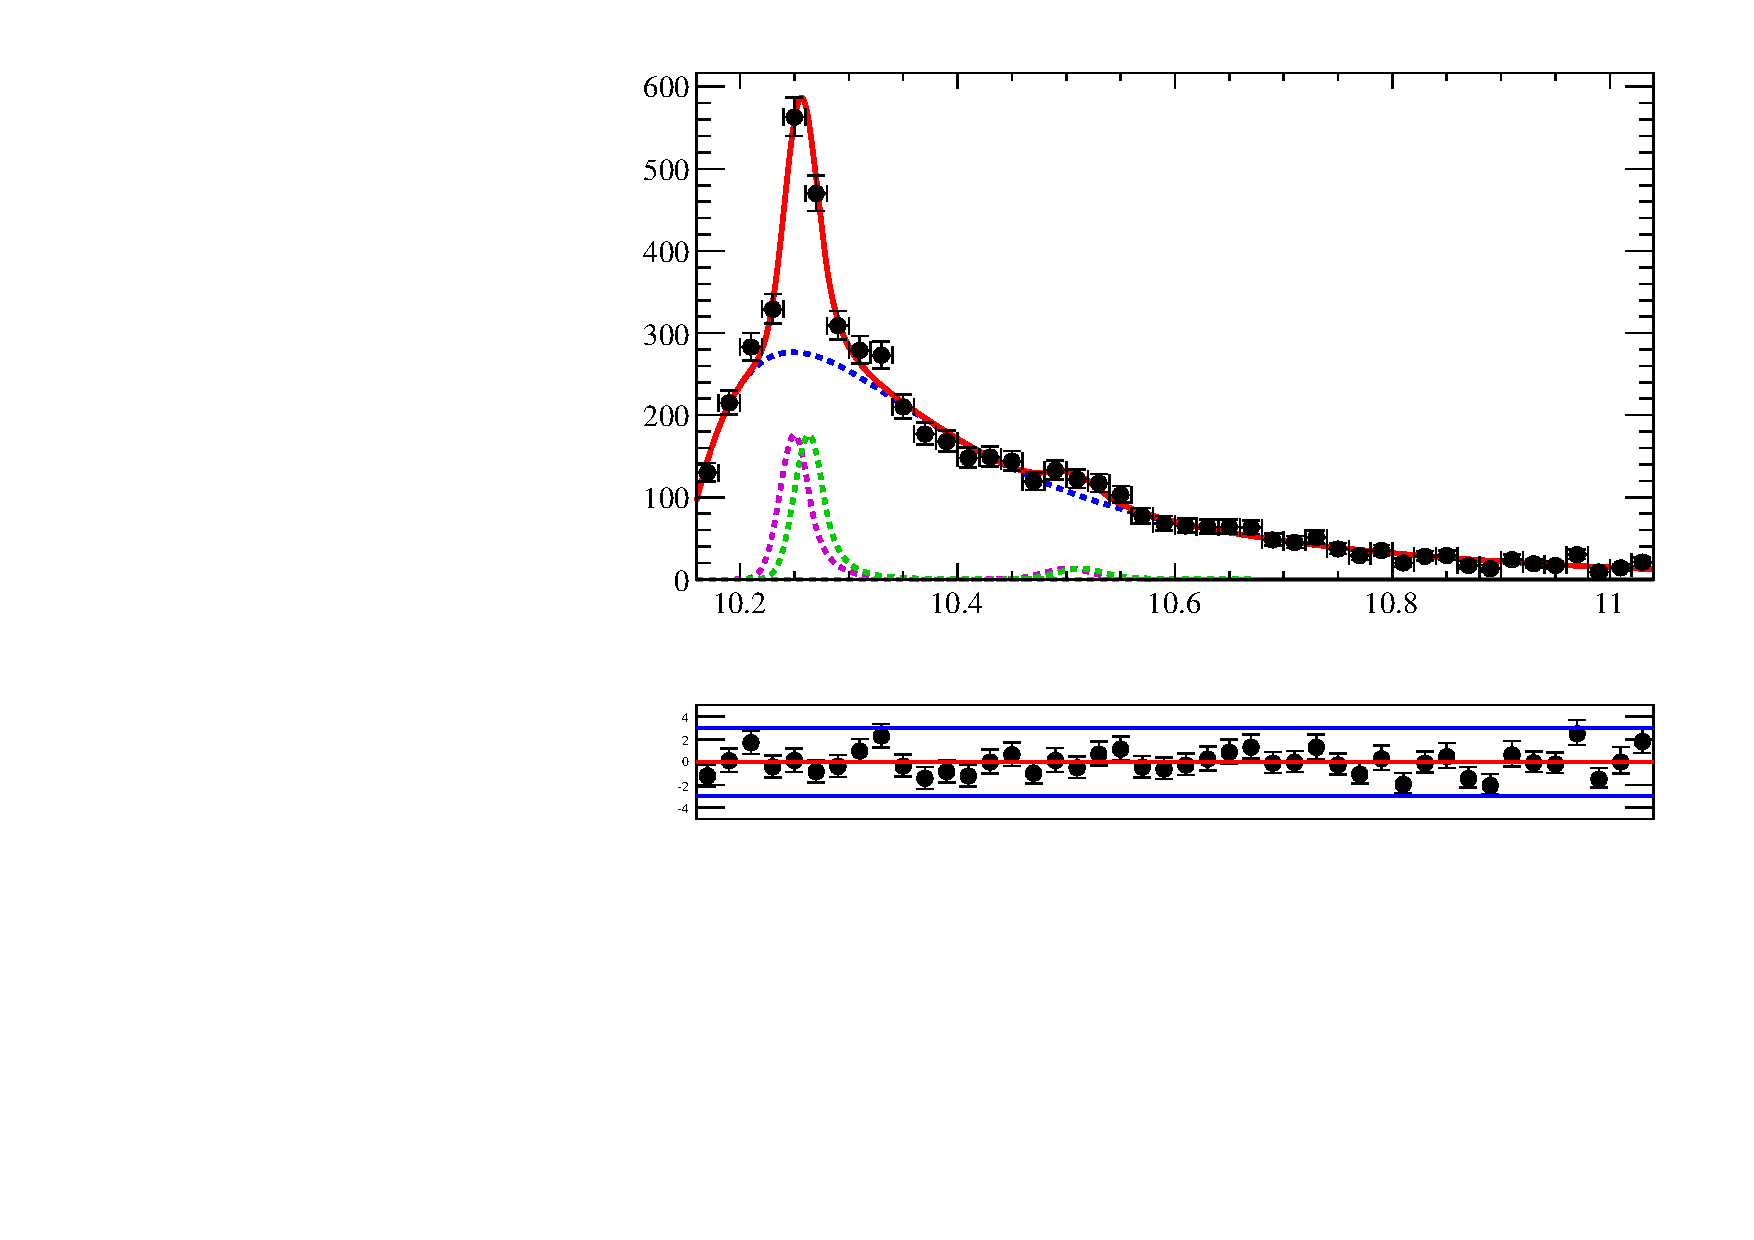
\includegraphics[width=50mm, height=40mm]{chib2s-fit/f2012_18_40}
    }
    
    \put(0,40){
      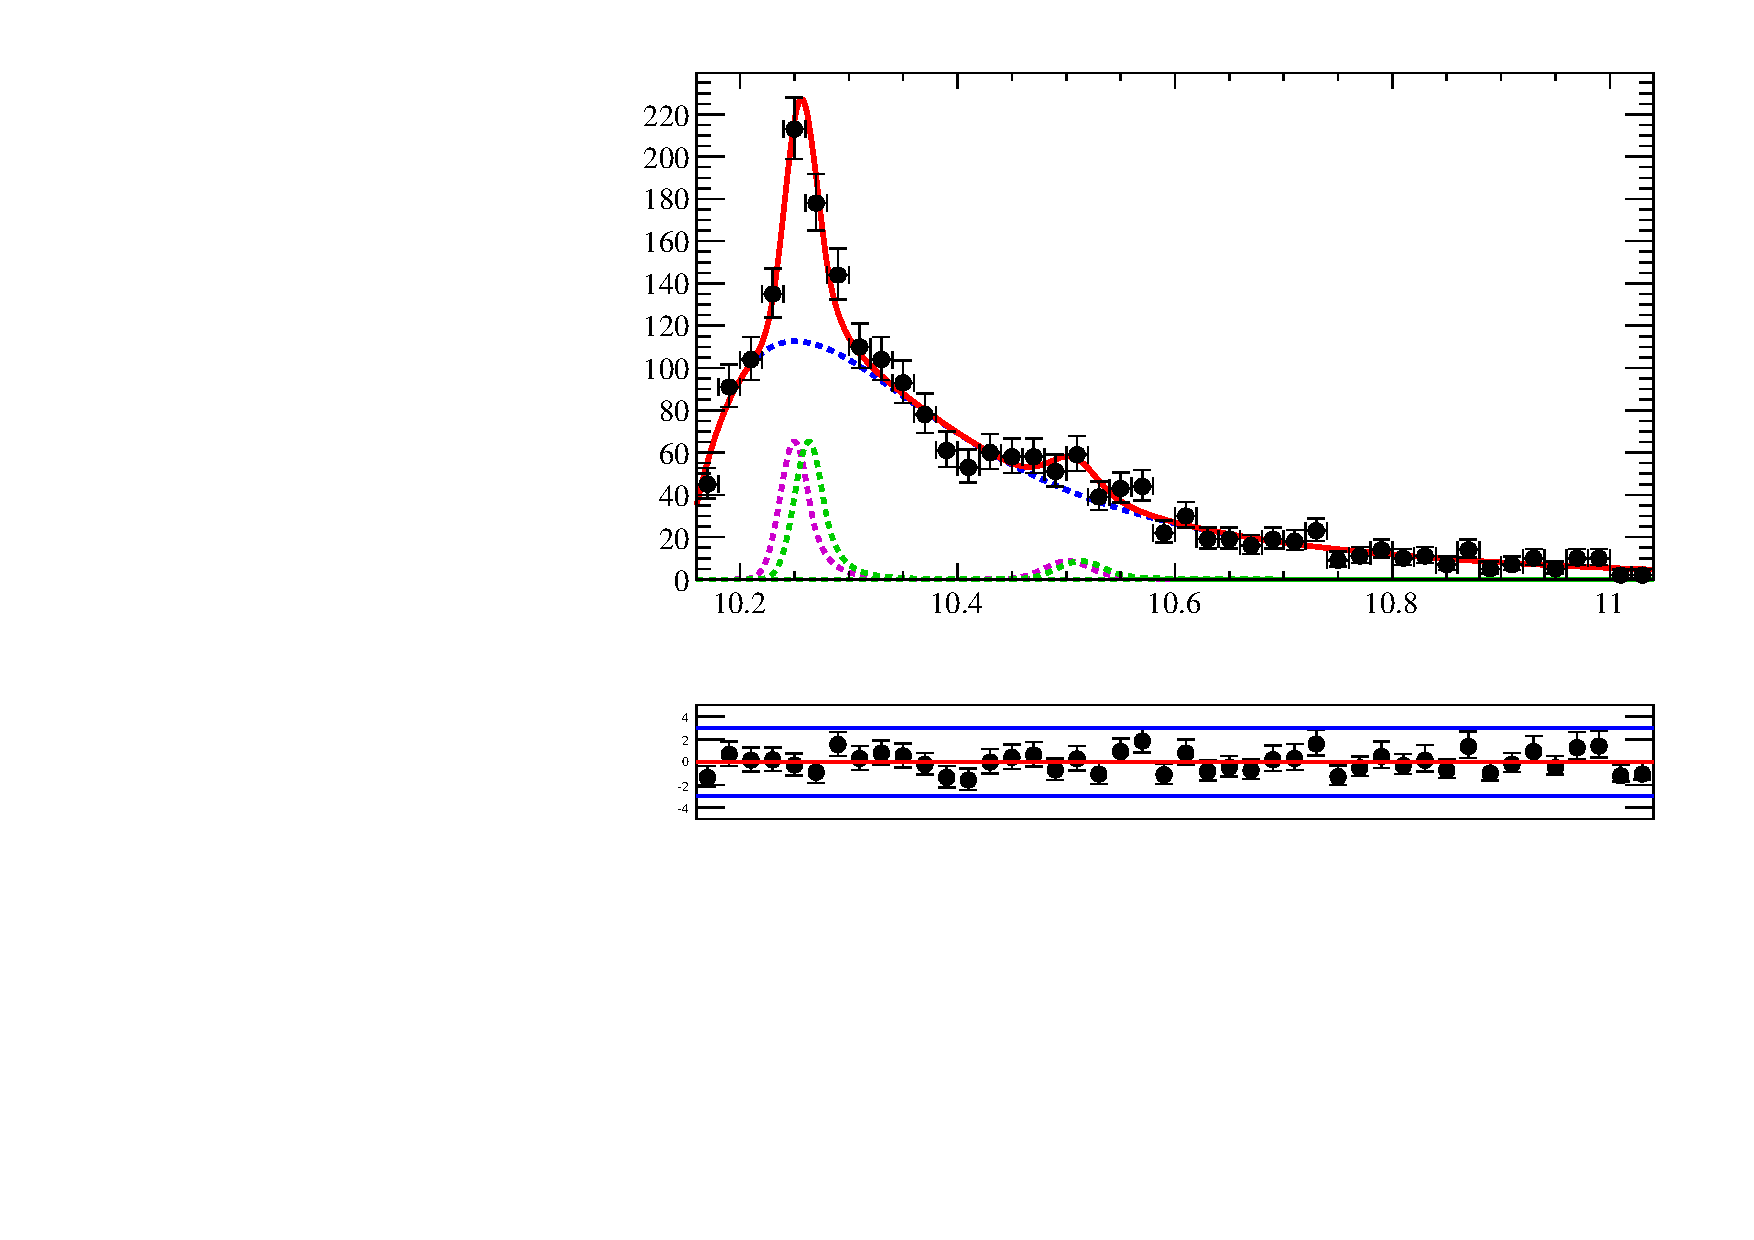
\includegraphics[width=50mm, height=40mm]{chib2s-fit/f2011_18_40}
    }

    \put(0,15){\tiny \begin{sideways}Candidates/(20\mevcc)\end{sideways}}
    \put(2,9){\tiny $m_{\mumu \gamma} - m_{\mumu} + m_{\Y2S}^{PDG} \left[\gevcc\right]$}
    \put(25,30){$\sqs=8 \tev$}
    \put(20,25){\tiny $ 18 < p_T^{\Y2S} < 40\gevc$}
    
    \put(0,55){\tiny \begin{sideways}Candidates/(20\mevcc)\end{sideways}}
    \put(2, 49){\tiny $m_{\mumu \gamma} - m_{\mumu} + m_{\Y2S}^{PDG} \left[\gevcc\right]$}
    \put(25,70){$\sqs=7 \tev$}
    \put(20,65){\tiny $18 < p_T^{\Y2S} < 40\gevc$}
    
    \put(15,75){\tiny \chibTwoP}
    \put(25,60){\tiny \chibThreeP}
    \put(15,35){\tiny \chibTwoP}
    \put(25,20){\tiny \chibThreeP}

    % \graphpaper[5](0,0)(50, 80)        
  \end{picture}
\column{.5\textwidth}
\begin{itemize}
\item One Crystal Ball (CB) for each $\chi_{b1,2}(2P,3P)$ state: 4 CB in total
\item Exclude the study of $\chi_{b0}$ due to its low radiative branching ratio.
\item Product of exponential and linear combination of polynomials  for combinatorial background.
\end{itemize}
\end{columns}
\end{frame}

\begin{frame}{$\chi_{b1,2}(2,3P) \to \TwoS \gamma$ fit model (2)}
\begin{columns}[T]
\column{.6\textwidth}
\begin{itemize}
\item Free parameters: $\mu_{\chi_{b1}(2P)}$, yields and background parameters.
\item Linked parameters for \chibone and \chibtwo signals:
    \begin{itemize}
    \item $\mu_{\chi_{b2}(2P)} = \mu_{\chi_{b1}(2P)} + \Delta m_{\chi_{b2}(2P)}^{PDG}$
    \item $\mu_{\chi_{b2}(3P)} = \mu_{\chi_{b1}(3P)} + \Delta m_{\chi_{b2}(3P)}^{theory}$
    \item $N_{\chi_{b}} = \lambda N_{\chi_{b1}} + (1-\lambda) N_{\chi_{b2}}$
    \item $\sigma_{\chi_{b2}} = \sigma_{\chi_{b1}}$
    \end{itemize}
\item Other linked parameters:    
    \begin{itemize}
        \item $\mu_{\chiboneThreeP} = \mu_{\chiboneOneP} + \Delta m_{\chi_{b1}(3P)}$ ($\Delta m_{\chi_{b1}(3P)}$ measured in this study)
    \end{itemize}
\item Fixed parameters from MC study:
    \begin{itemize}
    \item $\sigma_{\chiboneTwoP}$,  $\frac{\sigma_{\chiboneThreeP}}{\sigma_{\chiboneTwoP}}$
    \item $\alpha$ and $n$ parameters of CB.
    \end{itemize}
\end{itemize}
\column{.4\textwidth}
\resizebox{.9\textwidth}{!}{
\begin{tabular}{lrr}\toprule
 & \multicolumn{2}{c}{$\Upsilon(2S)$ transverse momentum intervals, \gevc}\\
 & \multicolumn{2}{c}{18 -- 40}\\
\cmidrule(r){2-3}
 & \multicolumn{1}{c}{\sqs = 7\tev} & \multicolumn{1}{c}{\sqs = 8\tev}\\
\midrule
$N_{\chibTwoP}$ & 237 $\pm$ 29 & 650 $\pm$ 50\\
$N_{\chibThreeP}$ & 50 $\pm$ 17 & 78 $\pm$ 26\\

\rule{0pt}{4ex}Background & 1830 $\pm$ 50 & 4600 $\pm$ 80\\

\rule{0pt}{4ex}$\mu_{\chiboneTwoP}, \mevcc$ & 10,249.1 $\pm$ 2.2 & 10,249.9 $\pm$ 1.3\\
$\sigma_{\chiboneTwoP}, \mevcc$ & 13.0 & 13.3\\
$\sigma_{\chi_{b1}(3P)} / \sigma_{\chi_{b1}(2P)}$ & 1.65 & 1.65\\

\rule{0pt}{4ex}$\tau$ & -7.5 $\pm$ 0.8 & -7.7 $\pm$ 0.5\\
$c_0$ & 0.431 $\pm$ 0.027 & 0.435 $\pm$ 0.016\\
$c_1$ & -2.07 $\pm$ 0.09 & -2.12 $\pm$ 0.05\\
$c_2$ & 0.79 $\pm$ 0.36 & 0.79 $\pm$ 0.17\\

\rule{0pt}{4ex}$\chi^2 / n.d.f$ & 0.98 & 1.35\\
\bottomrule
\end{tabular}
} % scalebox

\bigskip
{\tiny \textcolor{blue}{The mass of $\chi_{b1}(2P)$  is about 6 \mevcc  less than value in PDG (10.25546 \gevcc).}}
\end{columns}


\end{frame}

\begin{frame}{Mass of \chiboneTwoP in $\chib \to \TwoS \gamma$ decay}
\begin{center}
\setlength{\unitlength}{1mm}
\begin{picture}(70,50)
  %
\put(0,0){
  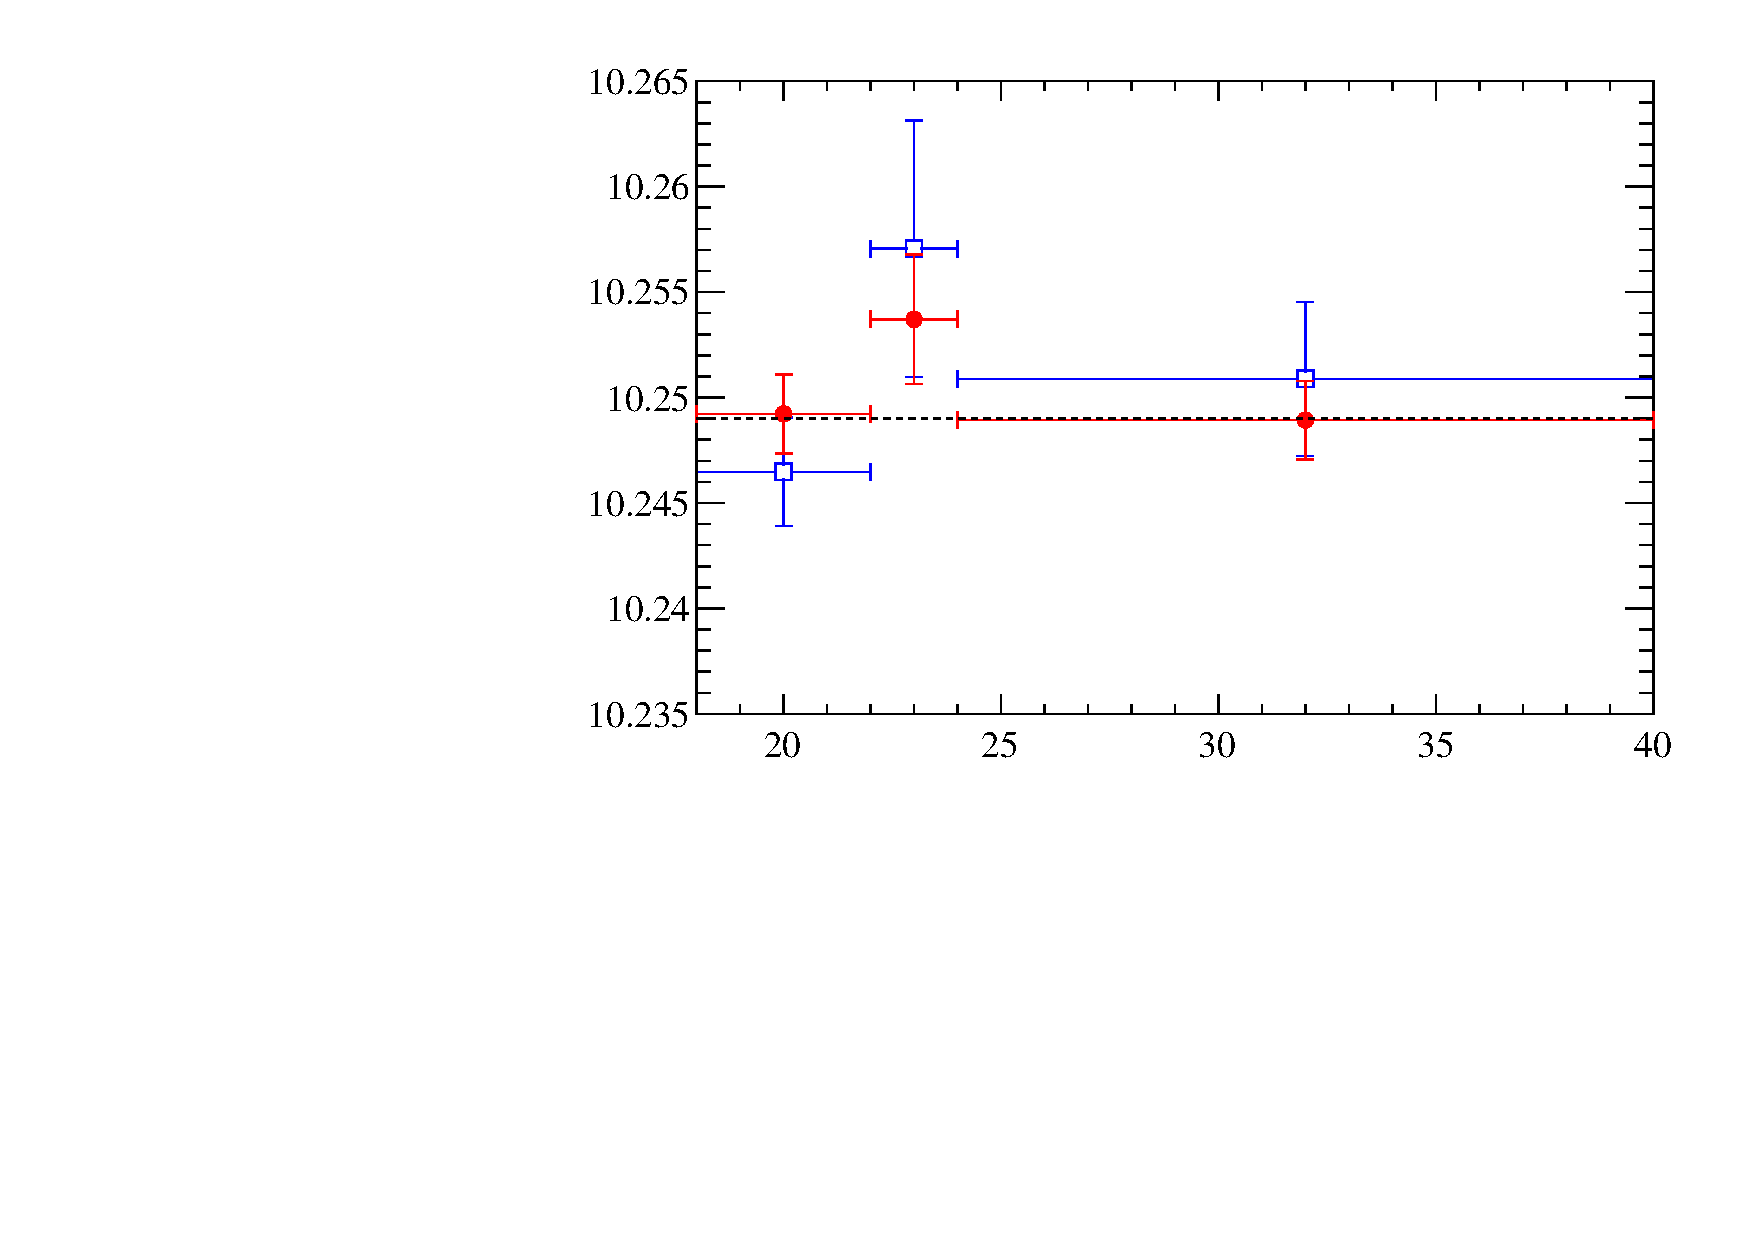
\includegraphics[width=70mm, height=50mm]{chib2s-m/m2p_2s}
}

\put(27, 40){\textcolor{blue}{\sqs=7\tev}, \textcolor{red}{\sqs=8\tev}}
\put(0,12){\begin{sideways}\chiboneTwoP mass \gevcc\end{sideways}}
\put(20,1){$p_T^{\Y2S} \left[\gevc\right]$}

\end{picture}
\end{center}

In the following, this mass was fixed to $10.249\gevcc$  which is the value
measured on the combined 2011 and 2012 datasets. A systematic uncertainty due
to this assumption has been assigned.


\end{frame}


\begin{frame}{$\chi_b$ yields in $\chi_b \to \TwoS \gamma$ decays}
  \setlength{\unitlength}{1mm}
  \centering
  \scalebox{0.7}{
  \begin{picture}(150,60)
    \put(0,0){
      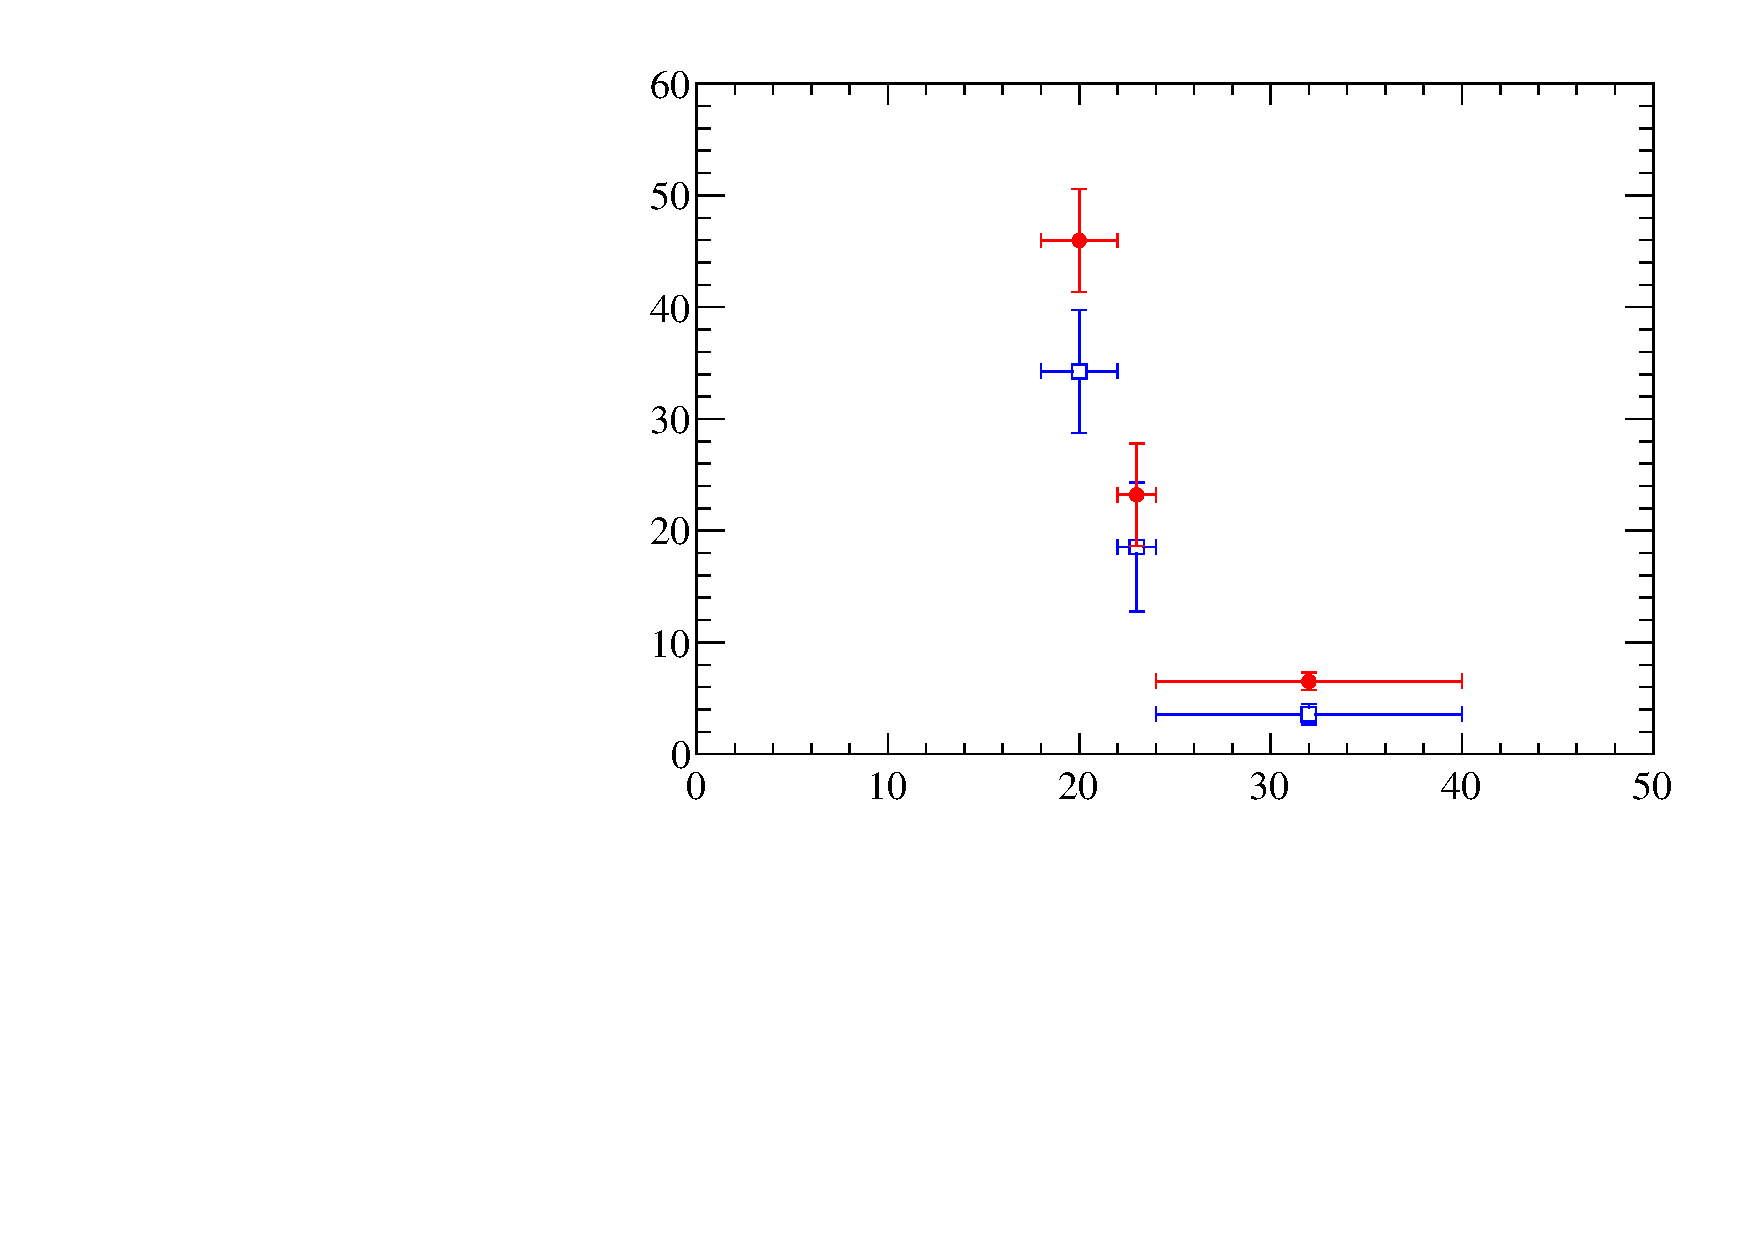
\includegraphics[width=75mm, height=60mm]{chib2s-yields/N2P_scaledbylum}
    }
    \put(75,0){
      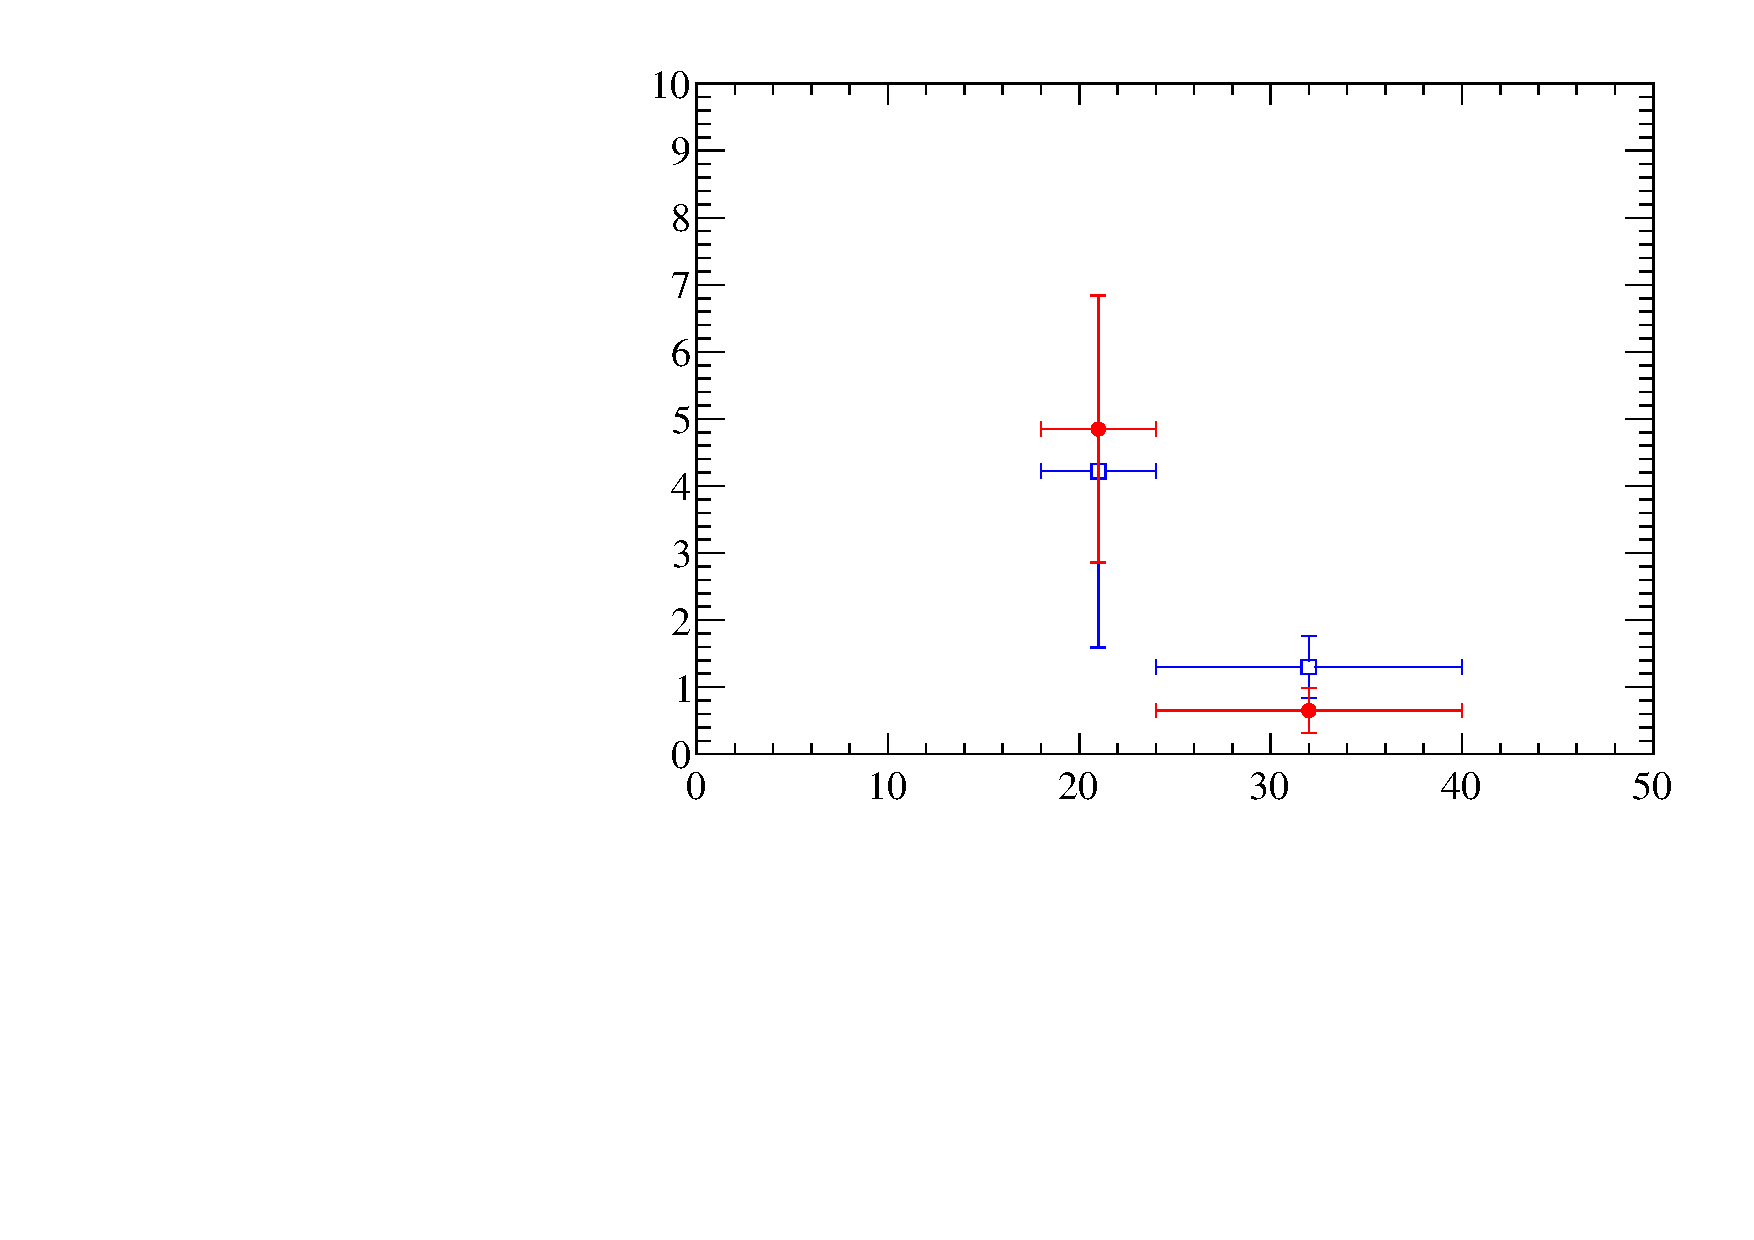
\includegraphics[width=75mm, height=60mm]{chib2s-yields/N3P_scaledbylum}
    }


    \put(2,25){\begin{sideways}Events\end{sideways}}
    \put(35,2){$p_T^{\Y2S} \left[\gevc\right]$}
    \put(55,50){$\chibTwoP$}

    \put(77,25){\begin{sideways}Events\end{sideways}}
    \put(110,2){$p_T^{\Y2S} \left[\gevc\right]$}
    \put(130,50){$\chibThreeP$}


    \put(50,45){\textcolor{blue}{\sqs=7\tev}}
    \put(50,40){\textcolor{red}{\sqs=8\tev}}
    \put(45,45){
      
\includegraphics[width=3mm, height=2mm]{bsf}
    }
    \put(45,40){
      
\includegraphics[width=3mm, height=2mm]{rco}
    }

    \put(125,45){\textcolor{blue}{\sqs=7\tev}}
    \put(125,40){\textcolor{red}{\sqs=8\tev}}
    \put(120,45){
      
\includegraphics[width=3mm, height=2mm]{bsf}
    }
    \put(120,40){
      
\includegraphics[width=3mm, height=2mm]{rco}
    }

  % \graphpaper[5](0,0)(75, 60)
  \end{picture}
}
\begin{center}
Yields normalized by bin width and luminosity.
\end{center}
\end{frame}


\begin{frame}{$\chi_{b1,2}(3P) \to \ThreeS \gamma$ fit model}
\begin{columns}[T]
\column{.5\textwidth}
  \centering
  \setlength{\unitlength}{1mm}
  \begin{picture}(50,80)
      %
    \put(0,0){
      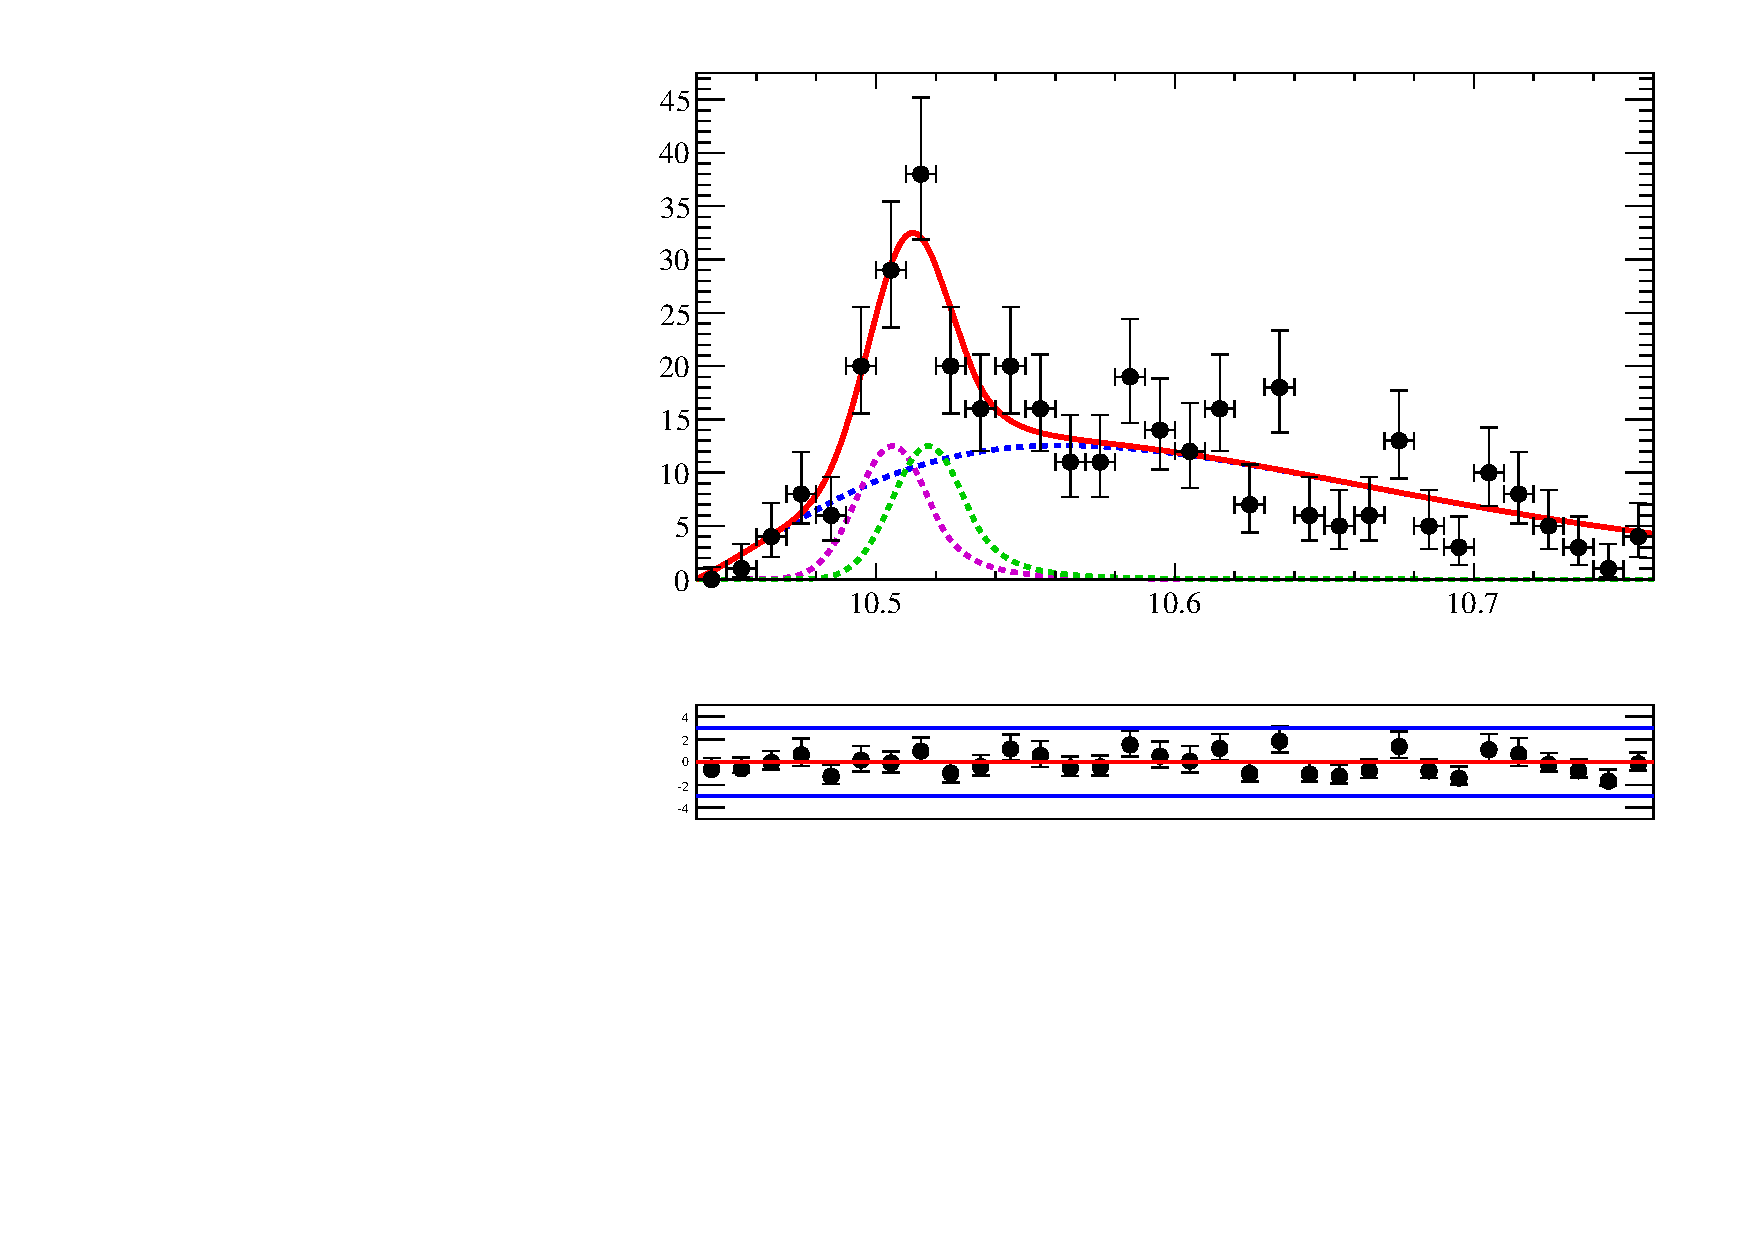
\includegraphics[width=50mm, height=40mm]{chib3s-fit/f2012_27_40}
    }
    
    \put(0,40){
      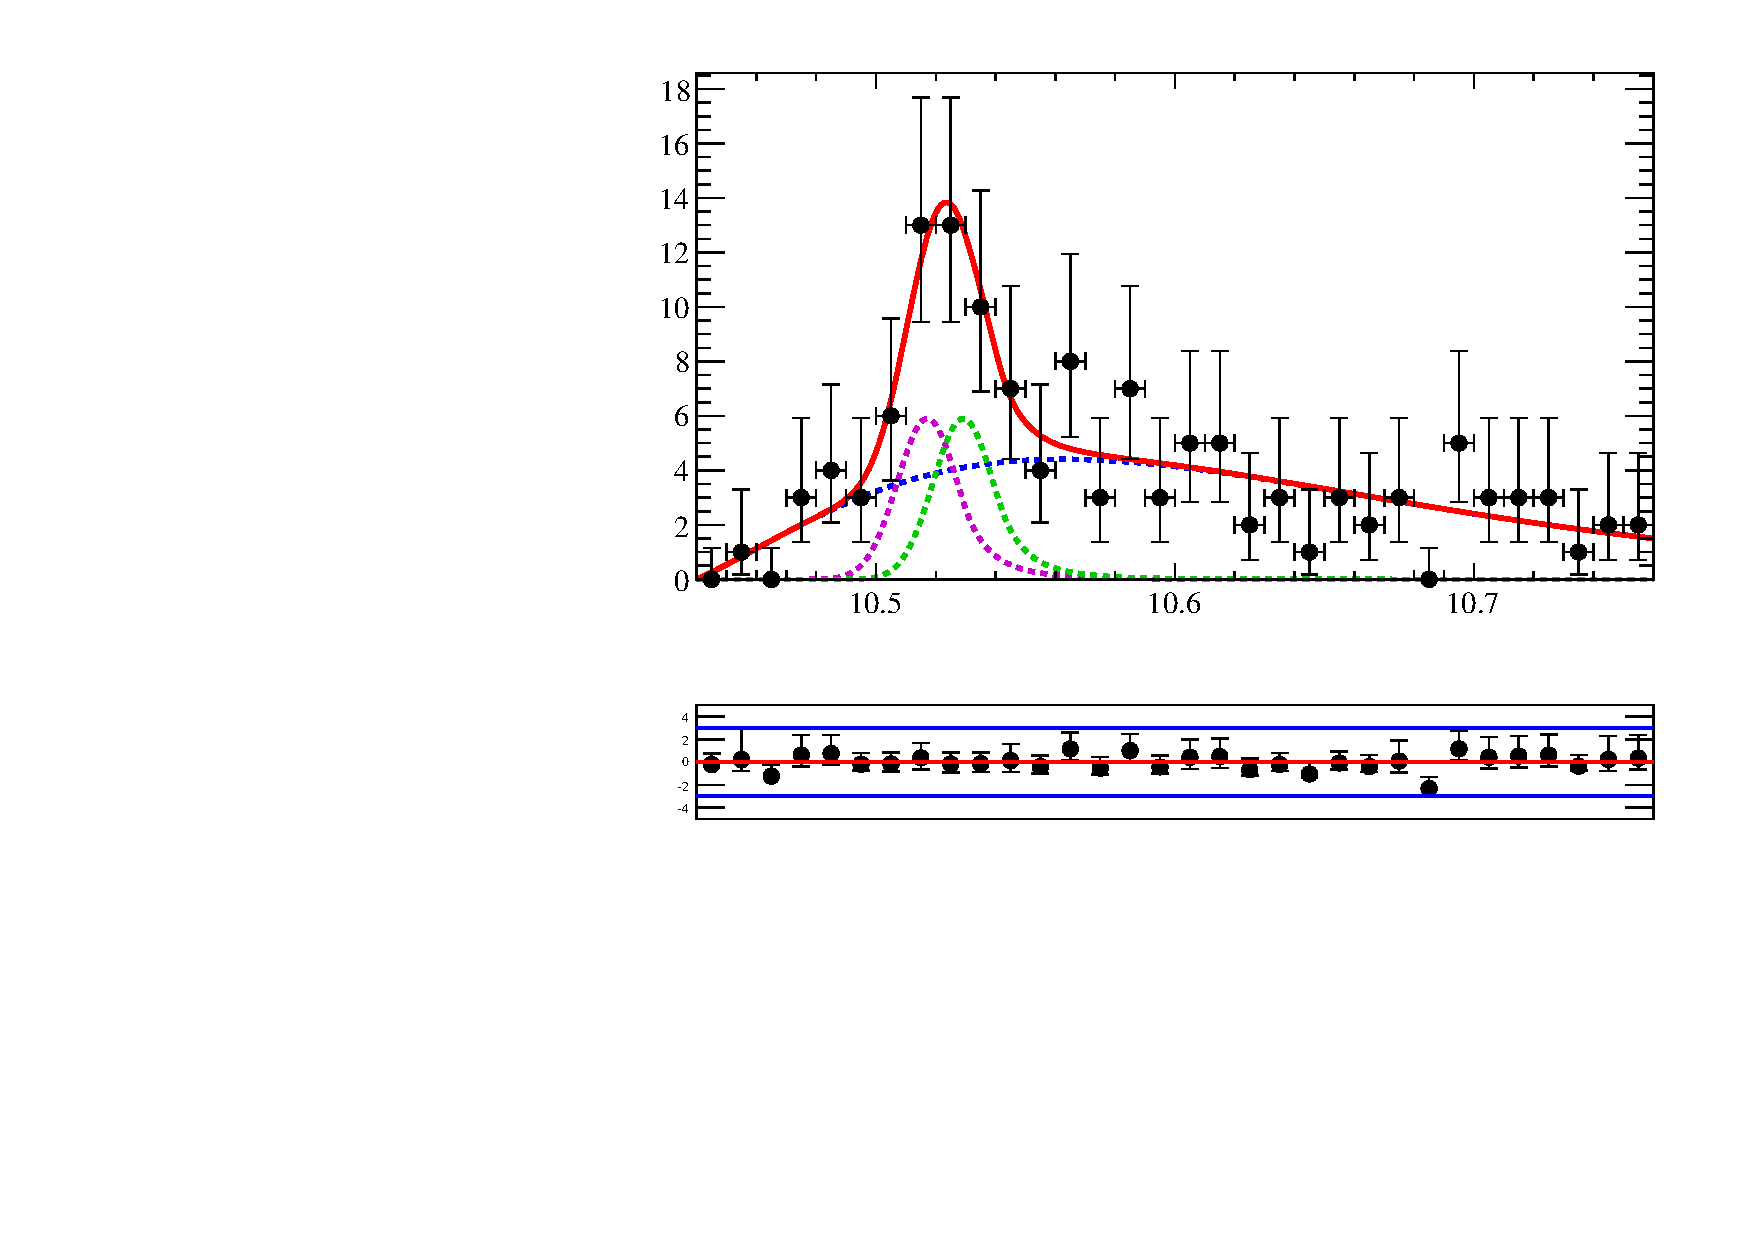
\includegraphics[width=50mm, height=40mm]{chib3s-fit/f2011_27_40}
    }

    \put(0,15){\tiny \begin{sideways}Candidates/(20\mevcc)\end{sideways}}
    \put(2,9){\tiny $m_{\mumu \gamma} - m_{\mumu} + m_{\Y3S}^{PDG} \left[\gevcc\right]$}
    \put(25,30){$\sqs=8\gev$}
    \put(20,25){\tiny $27 < p_T^{\Y3S} <  40 \gevc$}    
    
    \put(0,55){\tiny \begin{sideways}Candidates/(20\mevcc)\end{sideways}}
    \put(2, 49){\tiny $m_{\mumu \gamma} - m_{\mumu} + m_{\Y3S}^{PDG} \left[\gevcc\right]$}
    \put(25,70){$\sqs=7\gev$}     
    \put(20,65){\tiny $27 < p_T^{\Y3S} <  40 \gevc$}        
    
    \put(10,75){\tiny \chibThreeP}
    \put(10,35){\tiny \chibThreeP}

    % \graphpaper[5](0,0)(50, 80)        
  \end{picture}
\column{.5\textwidth}
\begin{itemize}
\item One Crystal Ball (CB) for each $\chi_{b1,2}(3P)$ state: 2 CB in total
\item Exclude the study of $\chi_{b0}$ due to its low radiative branching ratio.
\item Product of exponential and linear combination of polynomials  for combinatorial background.
\end{itemize}
\end{columns}
\end{frame}

\begin{frame}{$\chi_{b1,2}(3P) \to \ThreeS \gamma$ fit model (2)}
\begin{columns}[T]
\column{.5\textwidth}
\begin{itemize}
\item Free parameters: $\mu_{\chi_{b1}(3P)}$, $\sigma_{\chiboneThreeP}$, yields, background parameters.
\item Linked parameters for \chibone and \chibtwo signals:
    \begin{itemize}
    \item $\mu_{\chi_{b2}(3P)} = \mu_{\chi_{b1}(3P)} + \Delta m_{\chi_{b2}(3P)}^{theory}$
    \item $N_{\chi_{b}} = \lambda N_{\chi_{b1}} + (1-\lambda) N_{\chi_{b2}}$
    \item $\sigma_{\chi_{b2}} = \sigma_{\chi_{b1}}$
    \end{itemize}

\item Fixed parameters from MC study:
    \begin{itemize}
    \item $\alpha$ and $n$ parameters of CB.
    \end{itemize}
\end{itemize}
\column{.5\textwidth}
\resizebox{.9\textwidth}{!}{
\begin{tabular}{lrr}\toprule
 & \multicolumn{2}{c}{$\Upsilon(3S)$ transverse momentum intervals, \gevc}\\
 & \multicolumn{2}{c}{27 -- 40}\\
\cmidrule(r){2-3}
 & \sqs = 7\tev & \sqs = 8\tev\\
\midrule
$N_{\chibThreeP}$ & 31 $\pm$ 12 & 72 $\pm$ 16\\

\rule{0pt}{4ex}Background & 97 $\pm$ 14 & 283 $\pm$ 21\\

\rule{0pt}{4ex}$\mu_{\chiboneThreeP}, \mevcc$ & 10,517 $\pm$ 4 & 10,504.0 $\pm$ 2.5\\
$\sigma_{\chiboneThreeP}, \mevcc$ & 9 $\pm$ 6 & 8.3 $\pm$ 2.7\\

\rule{0pt}{4ex}$c_0$ & 0.52 $\pm$ 0.18 & 0.52 $\pm$ 0.09\\
$c_1$ & -0.42 $\pm$ 0.19 & -0.36 $\pm$ 0.10\\
$c_2$ & 1.3 $\pm$ 0.8 & -1.23 $\pm$ 0.18\\

\rule{0pt}{4ex}$\chi^2 / n.d.f$ & 0.38 & 1.09\\
\bottomrule
\end{tabular}
} % scalebox
%
\bigskip

In this study the mass of $\chi_{b1}(3P)$ was fixed to
\textcolor{blue}{10.508\gevcc} which is the value
measured on the combined 2011 and 2012 datasets.
\end{columns}


\end{frame}

\begin{frame}{Mass of \chiboneThreeP in $\chib \to \Y3S \gamma$ decay (1)}
\setlength{\unitlength}{1mm}
\centering

Systematic uncertanties due to unknown ratio and mass difference between $\chi_{b1}$ and $\chi_{b2}$ states:

\resizebox{0.5\textwidth}{!}{
\begin{picture}(80,60)
    %
    \put(0,0){
      \includegraphics*[width=80mm, height=60mm]{chib3s-lambda/m3p_lambda}
    }

     \put(0,15){\scriptsize \begin{sideways}Mass of \chiboneThreeP (\gevcc)\end{sideways}}
     \put(75,0){$\lambda$}

    \put(15,54){\includegraphics*[width=4mm, height=2mm]{blue}}
    \put(15,50){\includegraphics*[width=4mm, height=2mm]{red}}

    \put(20,54){\scriptsize \textcolor{blue}{$\Delta{m_{\chi_{b1,2}(3P)}} = 13\mevcc$}}
    \put(20,50){\scriptsize \textcolor{red}{$\Delta{m_{\chi_{b1,2}(3P)}} = 10\mevcc$}}
    % \put(48,140){\scriptsize \textcolor{cyan}{\sqs=7\tev (2010)}}
    
    % \put(15,169){\includegraphics*[width=4mm, height=2mm]{blue}}
    % \put(15,165){\includegraphics*[width=4mm, height=2mm]{red}}     

     % \graphpaper[5](0,0)(80, 60)
  \end{picture}
}
\begin{block}{}
\scriptsize
The mass is measured with different ratios ($\lambda$) and mass difference 
($\Delta{m_{\chi_{b1,2}(3P)}}$) between \chiboneThreeP and \chibtwoThreeP states.
The measurement is performed on the combined 2011 and 2012 datasets.
\end{block}

% \begin{alertblock}{}
% According to theory prediction, where this ratio is
% variates in range from 0.4 to 0.7, follows that \chiboneThreeP mass is in 
% the range between 10.504 and 10.514 \gevcc.
% \end{alertblock}

% In this study the mass of \chiboneOneP was fixed to \textcolor{blue}{9892} \mevcc.

\end{frame}
\begin{frame}{Mass of \chiboneThreeP in $\chib \to \Y3S \gamma$ decay (2)}
\begin{center}
The measured $m_{\chiboneThreeP}$=\textcolor{red}{$10{,}508\pm2\stat\pm8\syst\mevcc$} is consistent
with the mass measured in another study with converted photons ---
\textcolor{blue}{$10{,}510\pm3.0\stat^{+4.4}_{-3.4}\syst\mevcc$} (very preliminary results).
% 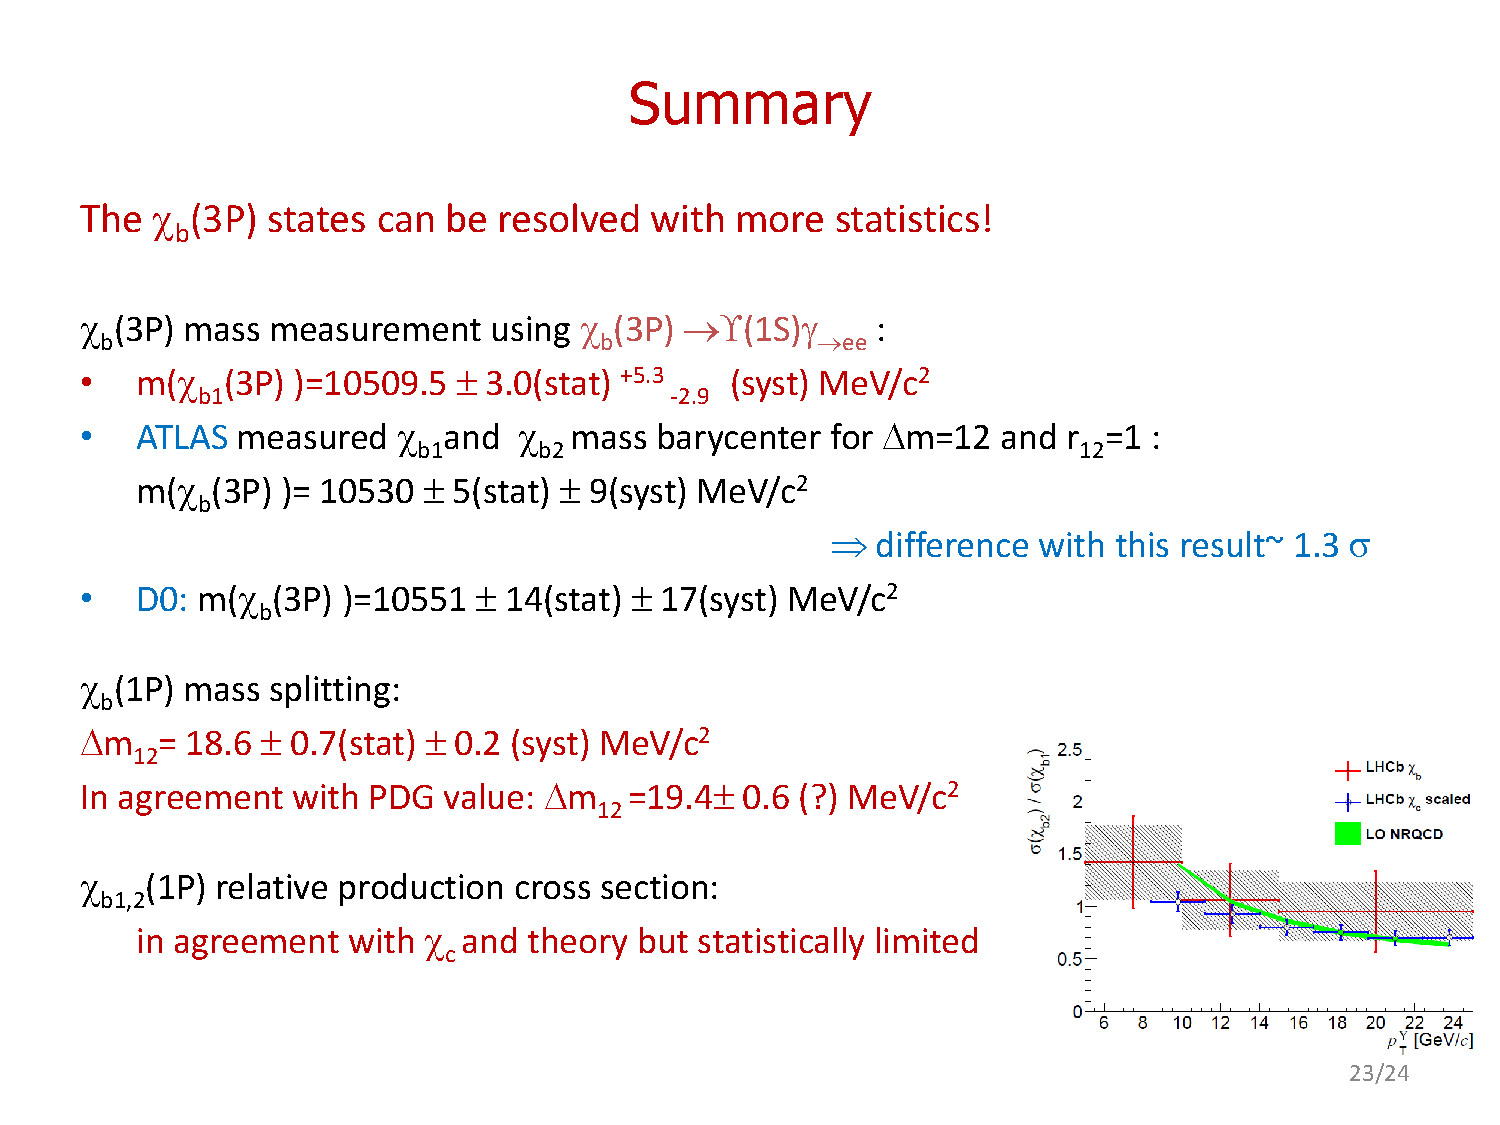
\includegraphics[width=85mm]{m3p-converted/converted}
\end{center}
\begin{itemize}
\item \atlas measured $\chi_{b1}$ and $\chi_{b2}$  mass barycenter for $m_{\chi_{b2}} - m_{\chi_{b1}}=12\mevcc$ and $\lambda=0.5$:
\textcolor{blue}{$m_{\chibThreeP} = 10{,}530\pm5\stat\pm9\syst\mevcc$}
\item D0: \textcolor{blue}{$m_{\chibThreeP} = 10{,}551\pm14\stat\pm17\syst\mevcc$}
\end{itemize}
\end{frame}

\begin{frame}{MC efficiency (1)}
\setlength{\unitlength}{1mm}
\begin{center}
MC true events $\chi_b(3P) \to \Y1S \gamma$ (other decays have the same shape)
\begin{picture}(70,50)
      %
    \put(0,0){
      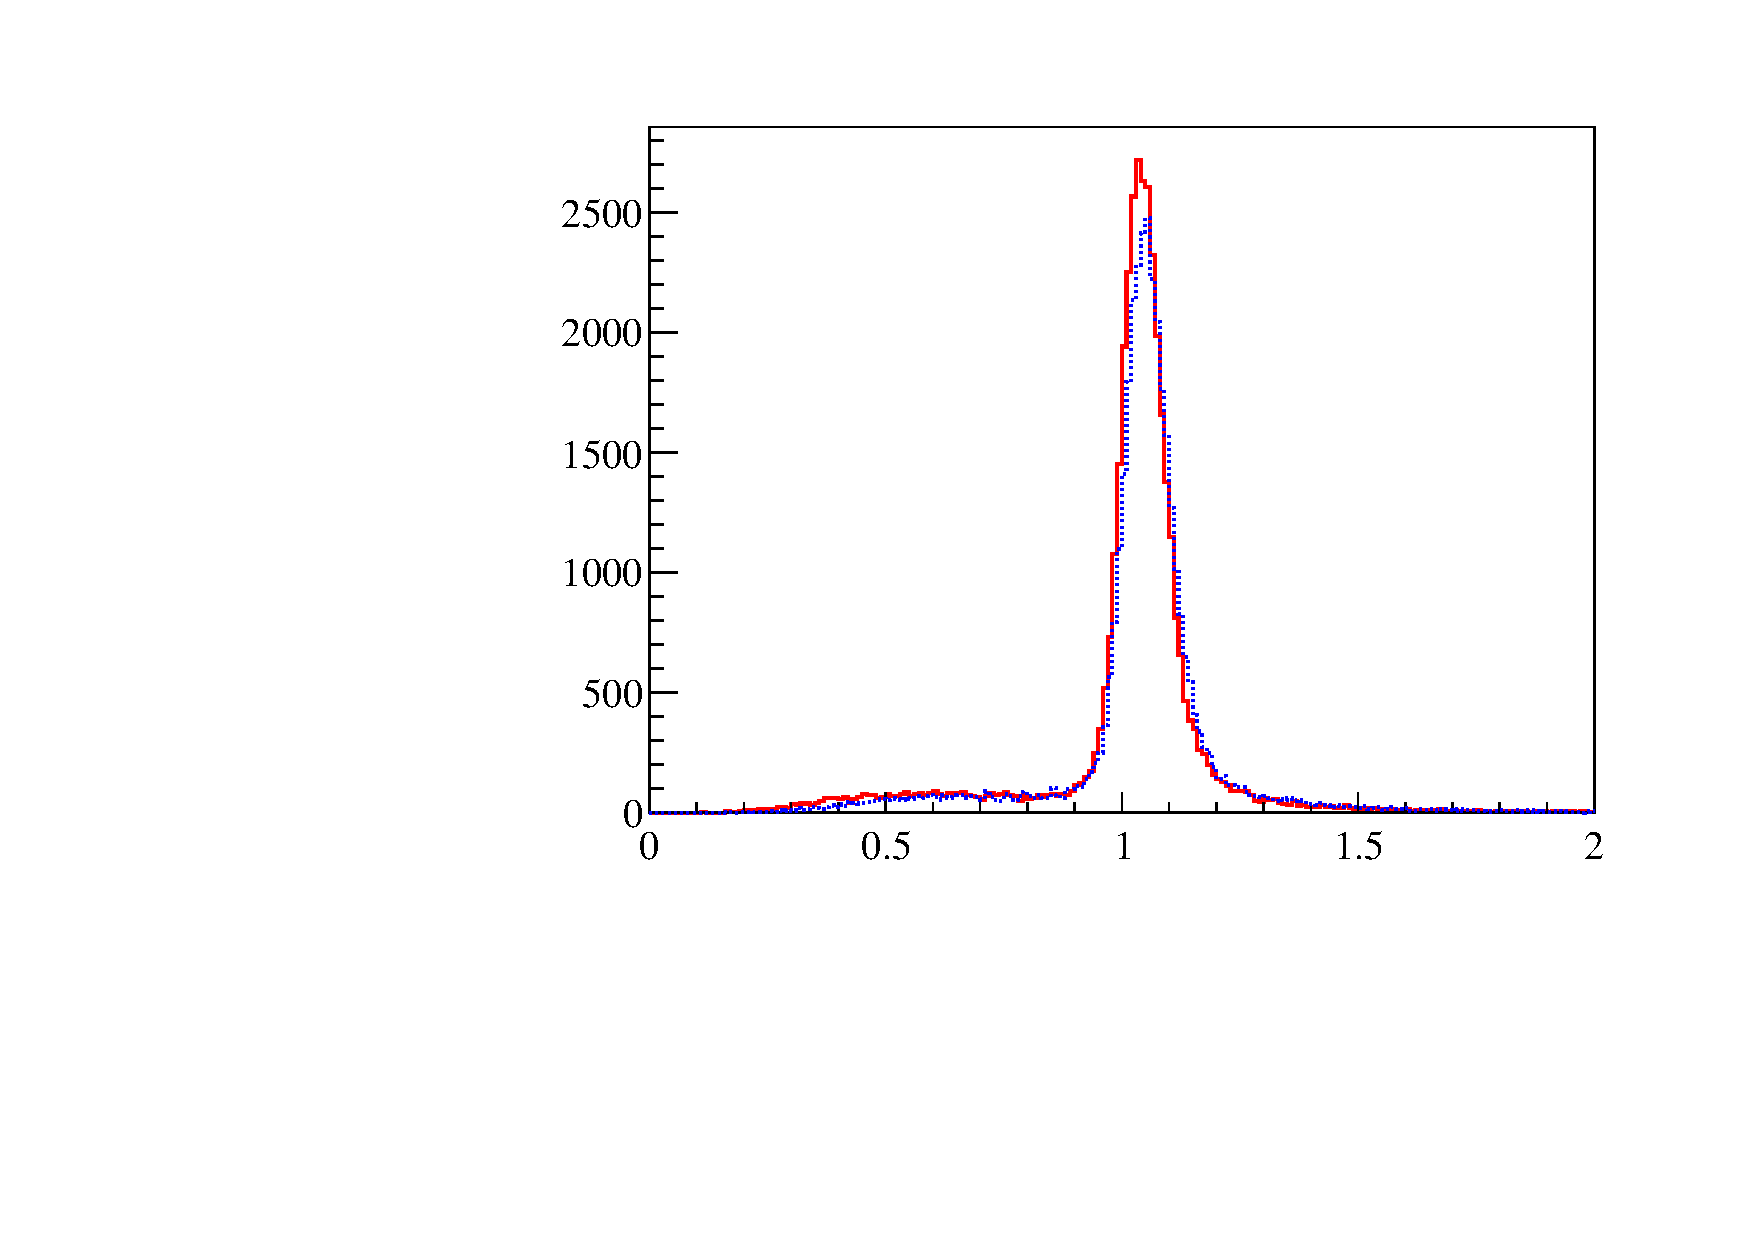
\includegraphics[width=70mm, height=50mm]{mc-fits/cb3_h}
    }
    
%    \put(0,40){
%      \includegraphics[width=50mm, height=40mm]{7.1-chib3s-fit/f2011_fix_27_None}
%    }

    \put(0,12){\begin{sideways}Candidates\end{sideways}}
    \put(20,0){$m_{\mumu \gamma} - m_{\mumu} \left[\gevcc\right]$}

%    
%    \put(0,55){\tiny \begin{sideways}Candidates/(20\mevcc)\end{sideways}}
%    \put(2, 49.5){\tiny $m_{\mumu \gamma} - m_{\mumu} + 10.3552 \left[\gevcc\right]$}
%    \put(25,70){$\sqrt{s} = 7 \gev$}     
%    \graphpaper[2](0,0)(70, 50)        
  \end{picture}
 \end{center}
 
\begin{alertblock}{}
\footnotesize
The flat left tails are due to photons which, although being correctly
associated to the \chib decay, are poorly reconstructed in the calorimeter. In
principle, these tails could be modeled in our fit to signal, but in practice
they will not be distinguishable from background. Therefore, the number of
\chib events for efficiency calculations \textbf{is not determined by simple event
counting but from a fit} where the tails are considered as background. $\Upsilon$
events are obtained by counting mc-true events.
\end{alertblock}

\end{frame}
\begin{frame}{Monte-Carlo photon reconstruction (2)}
Example of fits:
  \setlength{\unitlength}{1mm}
  \centering
  \scalebox{0.5}{
  \begin{picture}(225,120)
    \put(0,60){
      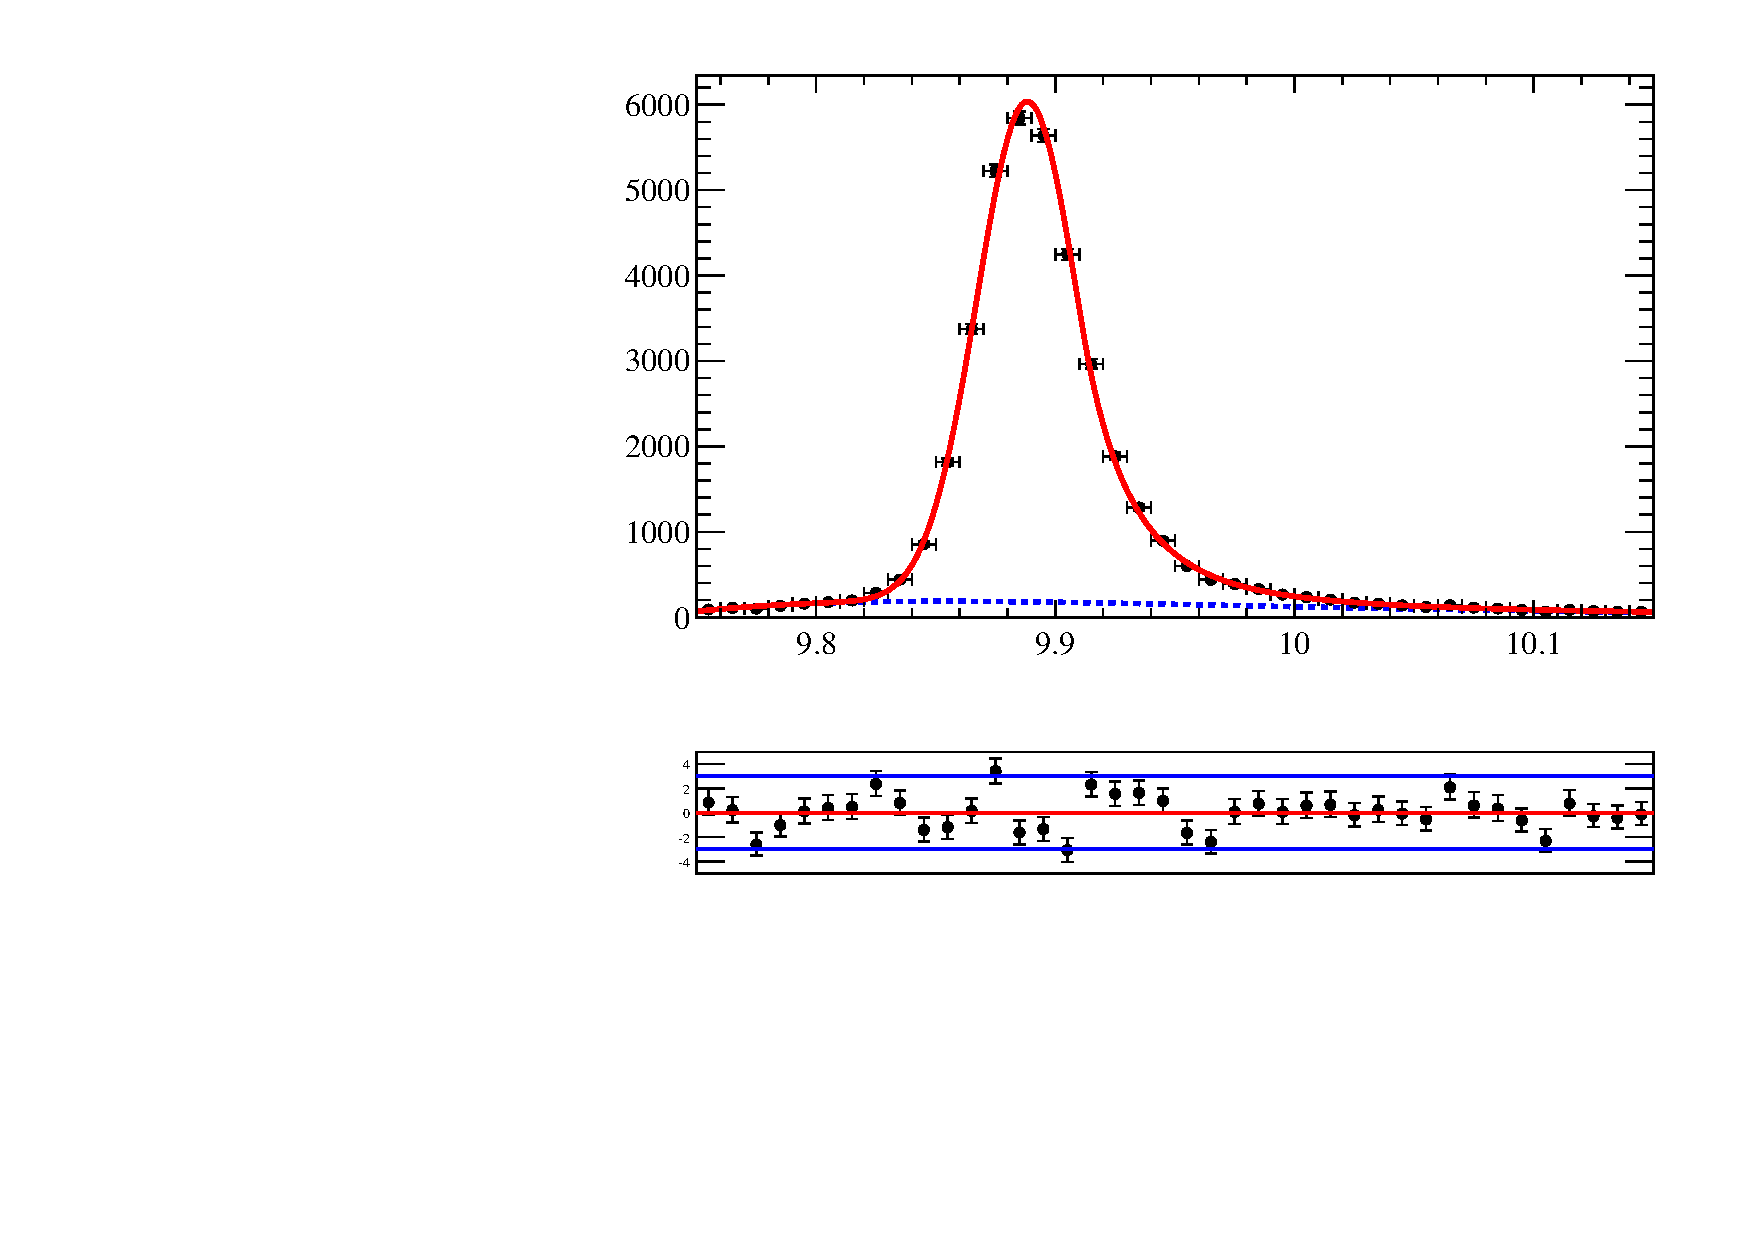
\includegraphics[width=75mm, height=60mm]{mc-fits-figs/cb11_6_40}
    }
    \put(42,114){\scriptsize $\chiboneOneP \to \Y1S \gamma$}
    \put(42,109){\scriptsize $6 < p_T^{\Y1S} < 40 \gevc$}
    \put(10,73){$m_{\mumu \gamma} - m_{\mumu} + m_{\Y1S}^{PDG} \left[\gevcc\right]$}
    \put(3,85){\scriptsize \begin{sideways}Candidates/(10\mevcc)\end{sideways}}    
    % \put(45,103){\scriptsize N = 34,330 $\pm$ 220}
    % \put(45,100){\scriptsize B = 5240 $\pm$ 140 (13.3 $\pm$ 0.4\%)}
    

    \put(75,60){
      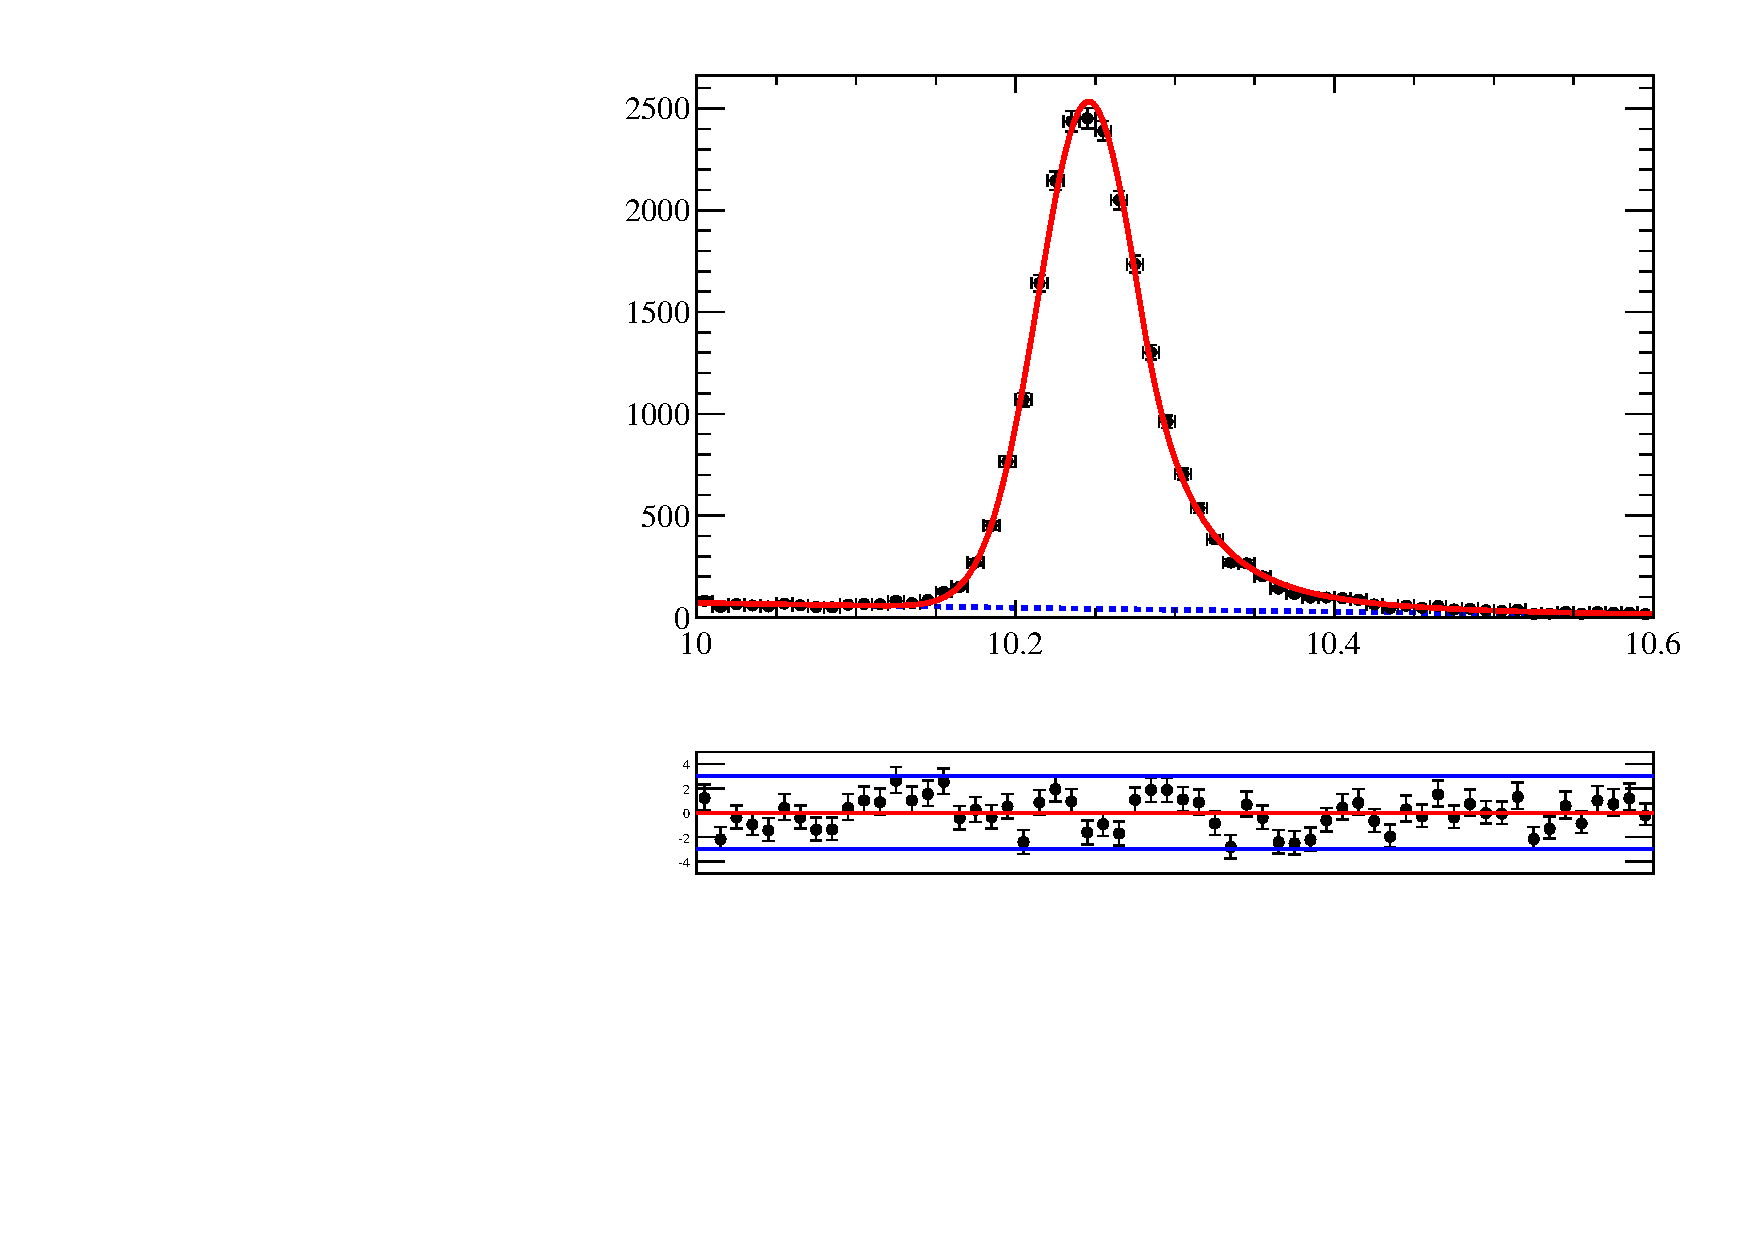
\includegraphics[width=75mm, height=60mm]{mc-fits-figs/cb12_6_40}
    }
    \put(117,114){\scriptsize $\chiboneTwoP \to \Y1S \gamma$}
    \put(117,109){\scriptsize $6 < p_T^{\Y1S} < 40 \gevc$}
    \put(85,73){$m_{\mumu \gamma} - m_{\mumu} + m_{\Y1S}^{PDG} \left[\gevcc\right]$}
    \put(78,85){\scriptsize \begin{sideways}Candidates/(10\mevcc)\end{sideways}}    
    % \put(120,103){\scriptsize N = 22,210 $\pm$ 170}
    % \put(120,100){\scriptsize B = 2290 $\pm$ 90 (9.3 $\pm$ 0.4\%)}
    

    \put(150,60){
      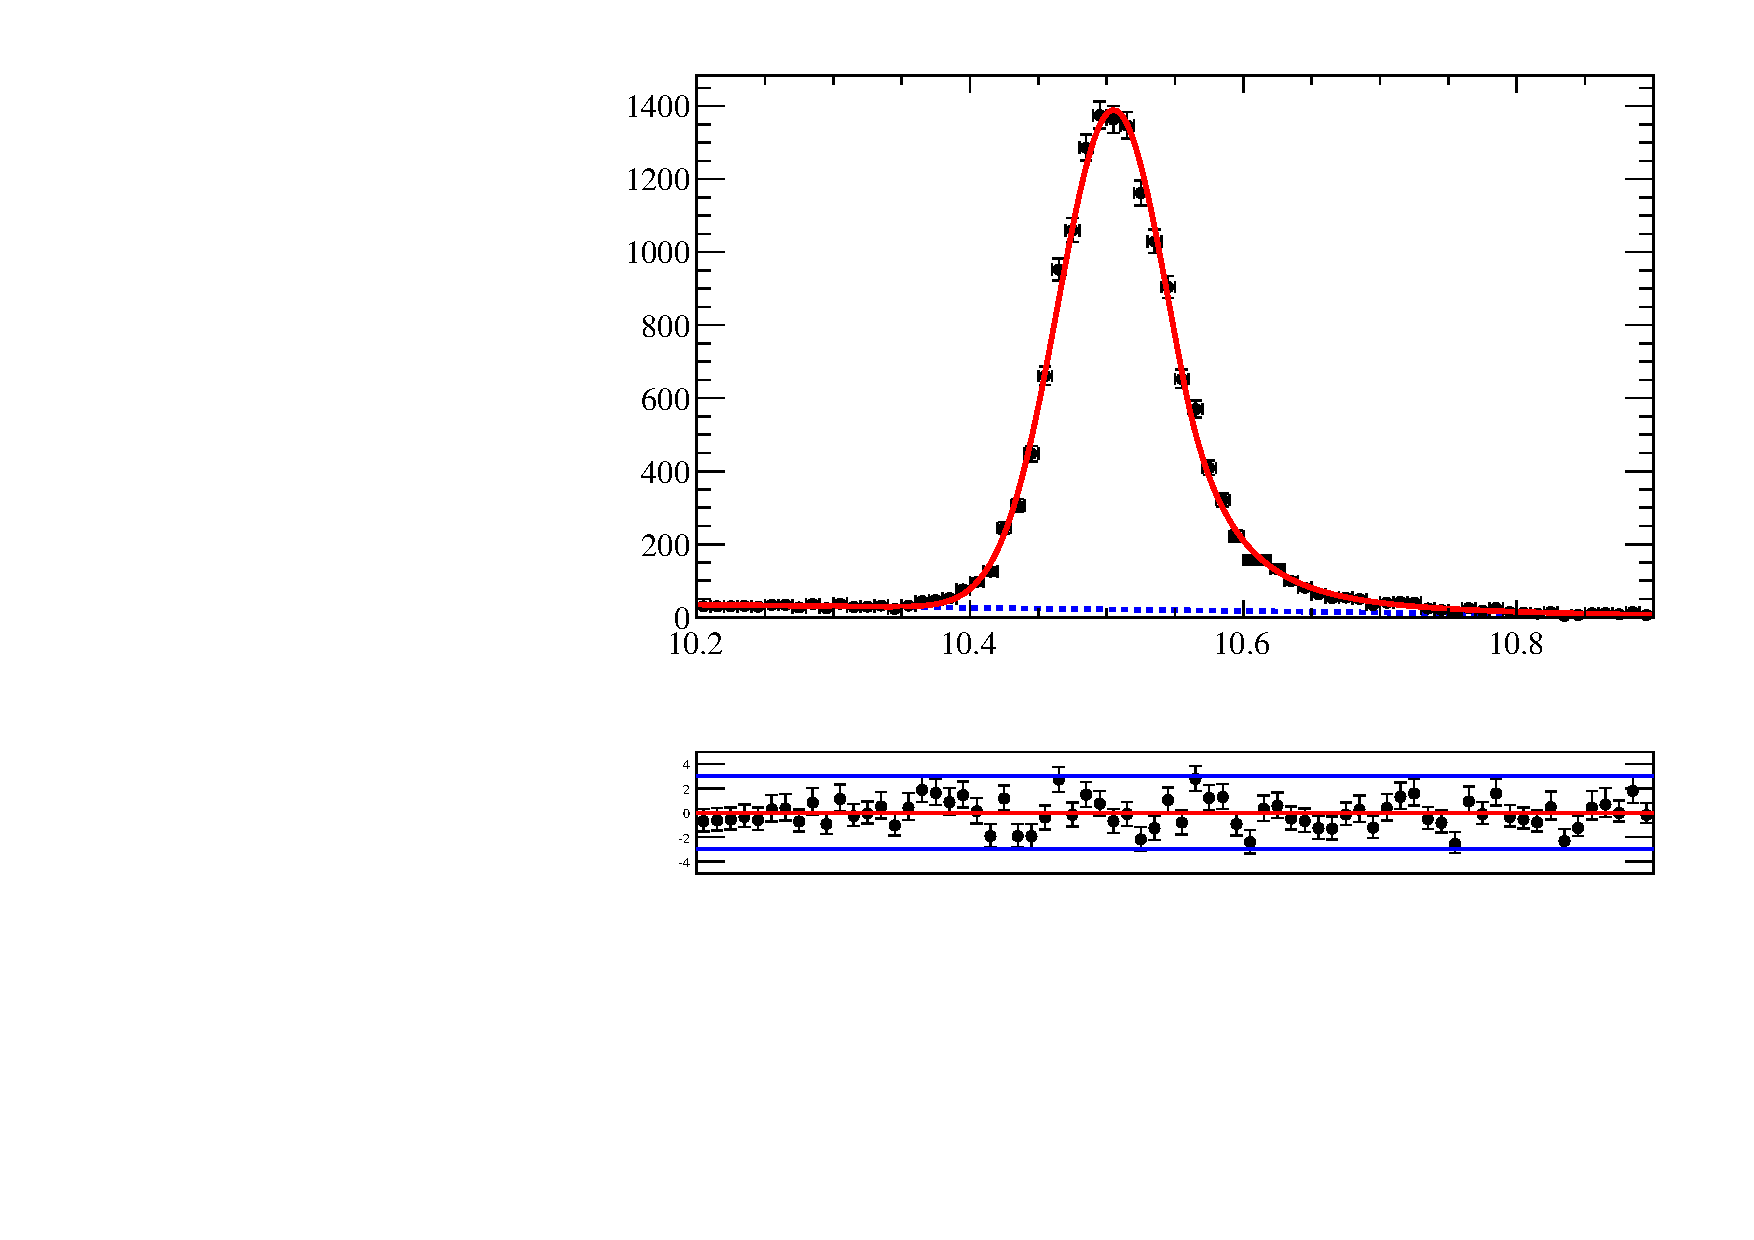
\includegraphics[width=75mm, height=60mm]{mc-fits-figs/cb13_6_40}
    }
    \put(192,114){\scriptsize $\chiboneThreeP \to \Y1S \gamma$}
    \put(192,109){\scriptsize $6 < p_T^{\Y1S} < 40 \gevc$}
    \put(160,73){$m_{\mumu \gamma} - m_{\mumu} + m_{\Y1S}^{PDG} \left[\gevcc\right]$}
    \put(153,85){\scriptsize \begin{sideways}Candidates/(10\mevcc)\end{sideways}}    
    % \put(195,103){\scriptsize N = 15,110 $\pm$ 130}
    % \put(195,100){\scriptsize B = 1360 $\pm$ 60 (8.26 $\pm$ 0.35\%)}
    

    \put(0,0){
      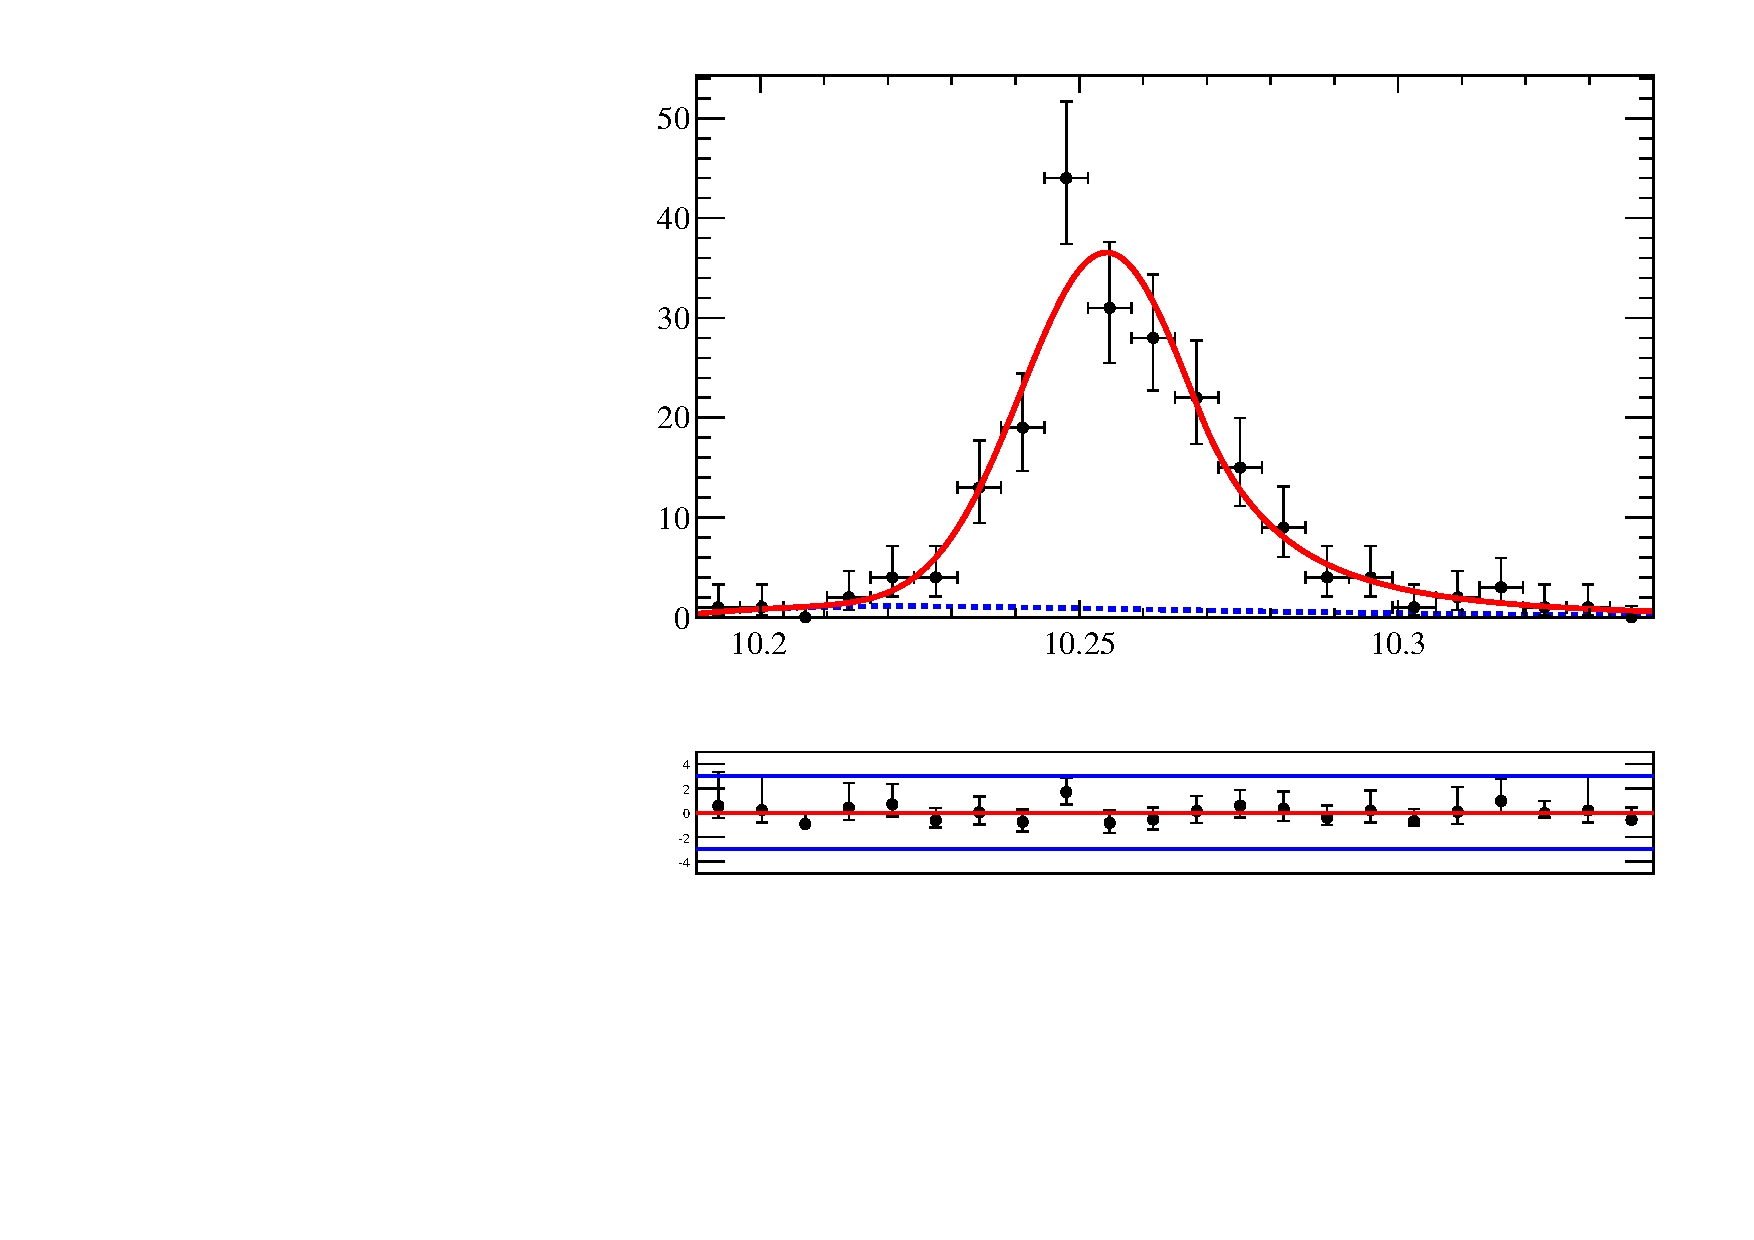
\includegraphics[width=75mm, height=60mm]{mc-fits-figs/cb12_18_40}
    }
    \put(42,54){\scriptsize $\chiboneTwoP \to \Y2S \gamma$}
    \put(42,49){\scriptsize $18 < p_T^{\Y2S} < 40 \gevc$}
    \put(10,13){$m_{\mumu \gamma} - m_{\mumu} + m_{\Y2S}^{PDG} \left[\gevcc\right]$}
    \put(3,25){\scriptsize \begin{sideways}Candidates/(10\mevcc)\end{sideways}}    
    % \put(45,43){\scriptsize N = 194 $\pm$ 21}
    % \put(45,40){\scriptsize B = 15 $\pm$ 17 (7 $\pm$ 8\%)}
    

    \put(75,0){
      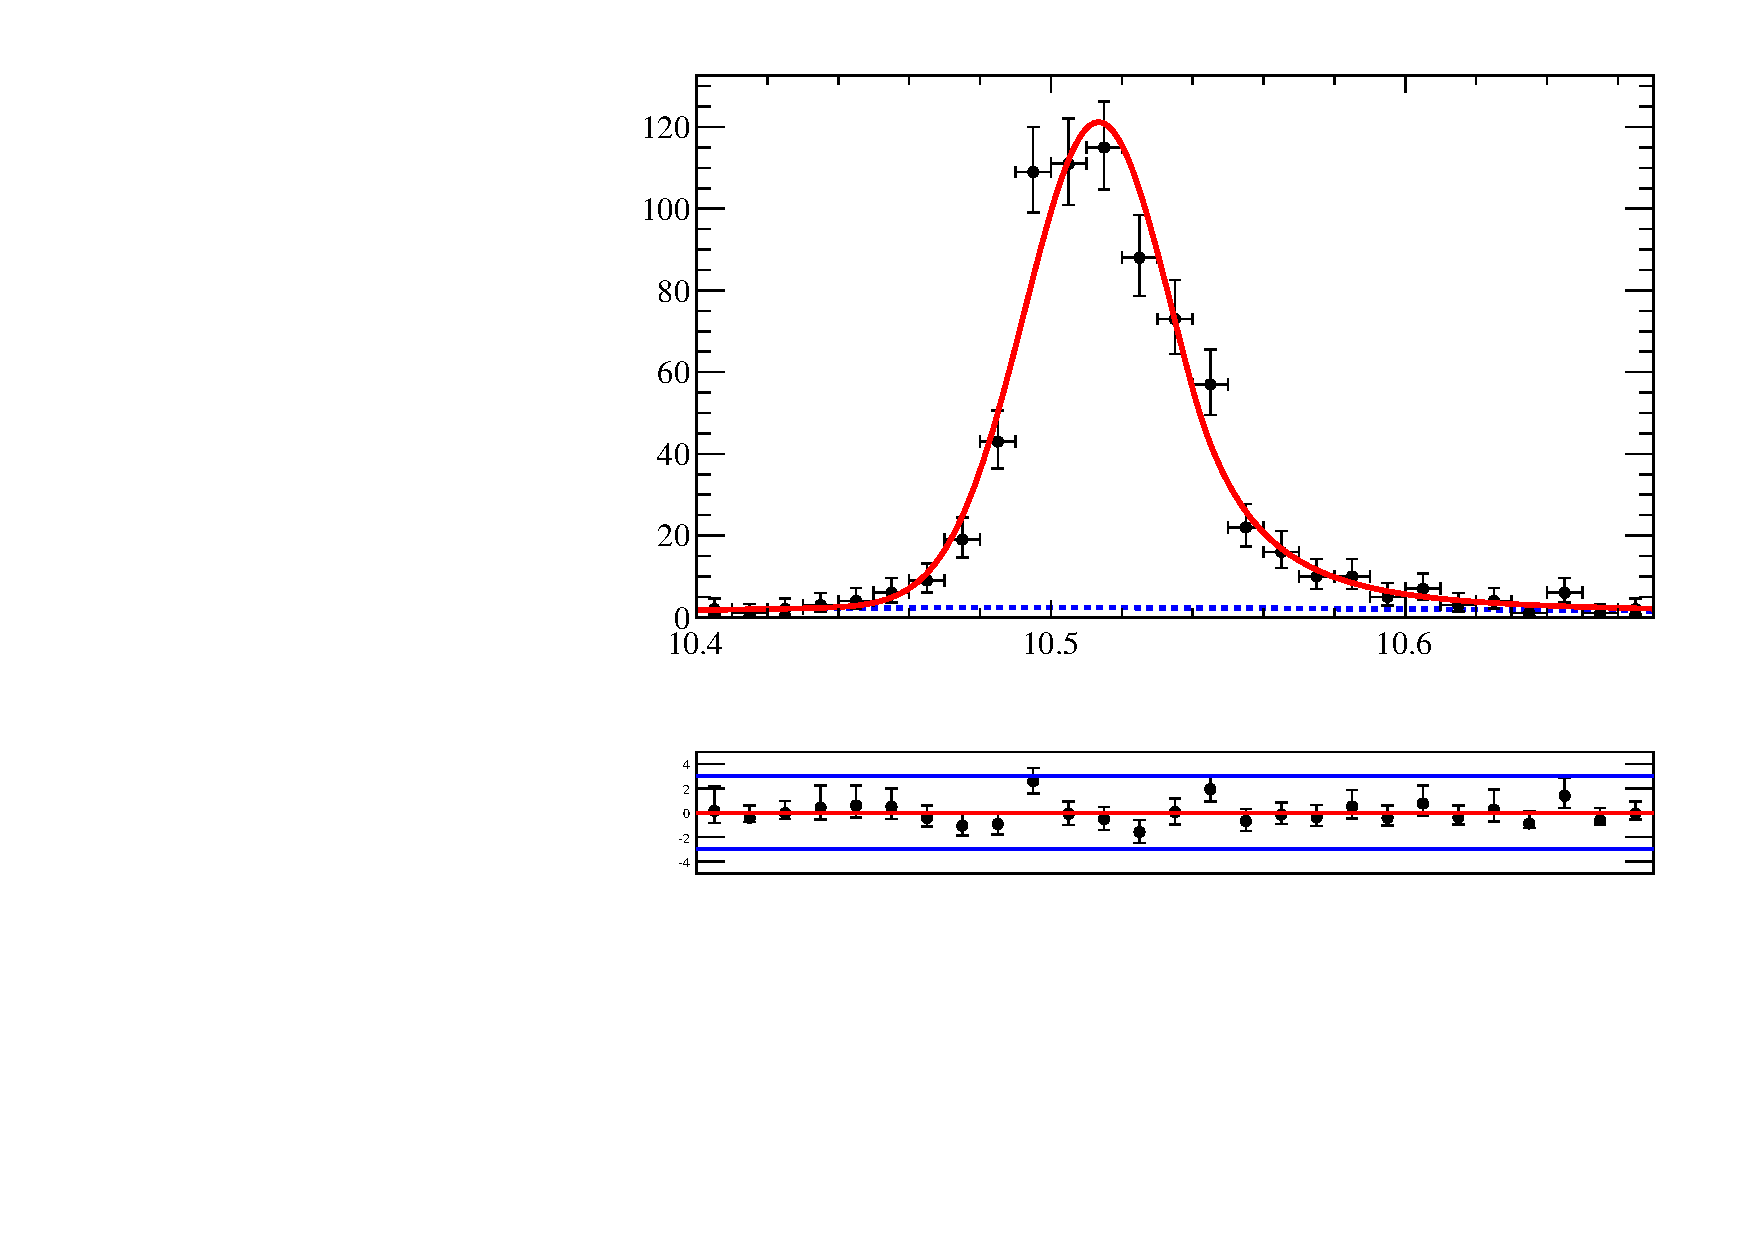
\includegraphics[width=75mm, height=60mm]{mc-fits-figs/cb13_18_40}
    }
    \put(117,54){\scriptsize $\chiboneThreeP \to \Y2S \gamma$}
    \put(117,49){\scriptsize $18 < p_T^{\Y2S} < 40 \gevc$}
    \put(85,13){$m_{\mumu \gamma} - m_{\mumu} + m_{\Y2S}^{PDG} \left[\gevcc\right]$}
    \put(78,25){\scriptsize \begin{sideways}Candidates/(10\mevcc)\end{sideways}}    
    % \put(120,43){\scriptsize N = 672 $\pm$ 32}
    % \put(120,40){\scriptsize B = 57 $\pm$ 21 (7.8 $\pm$ 2.9\%)}
    

    \put(150,0){
      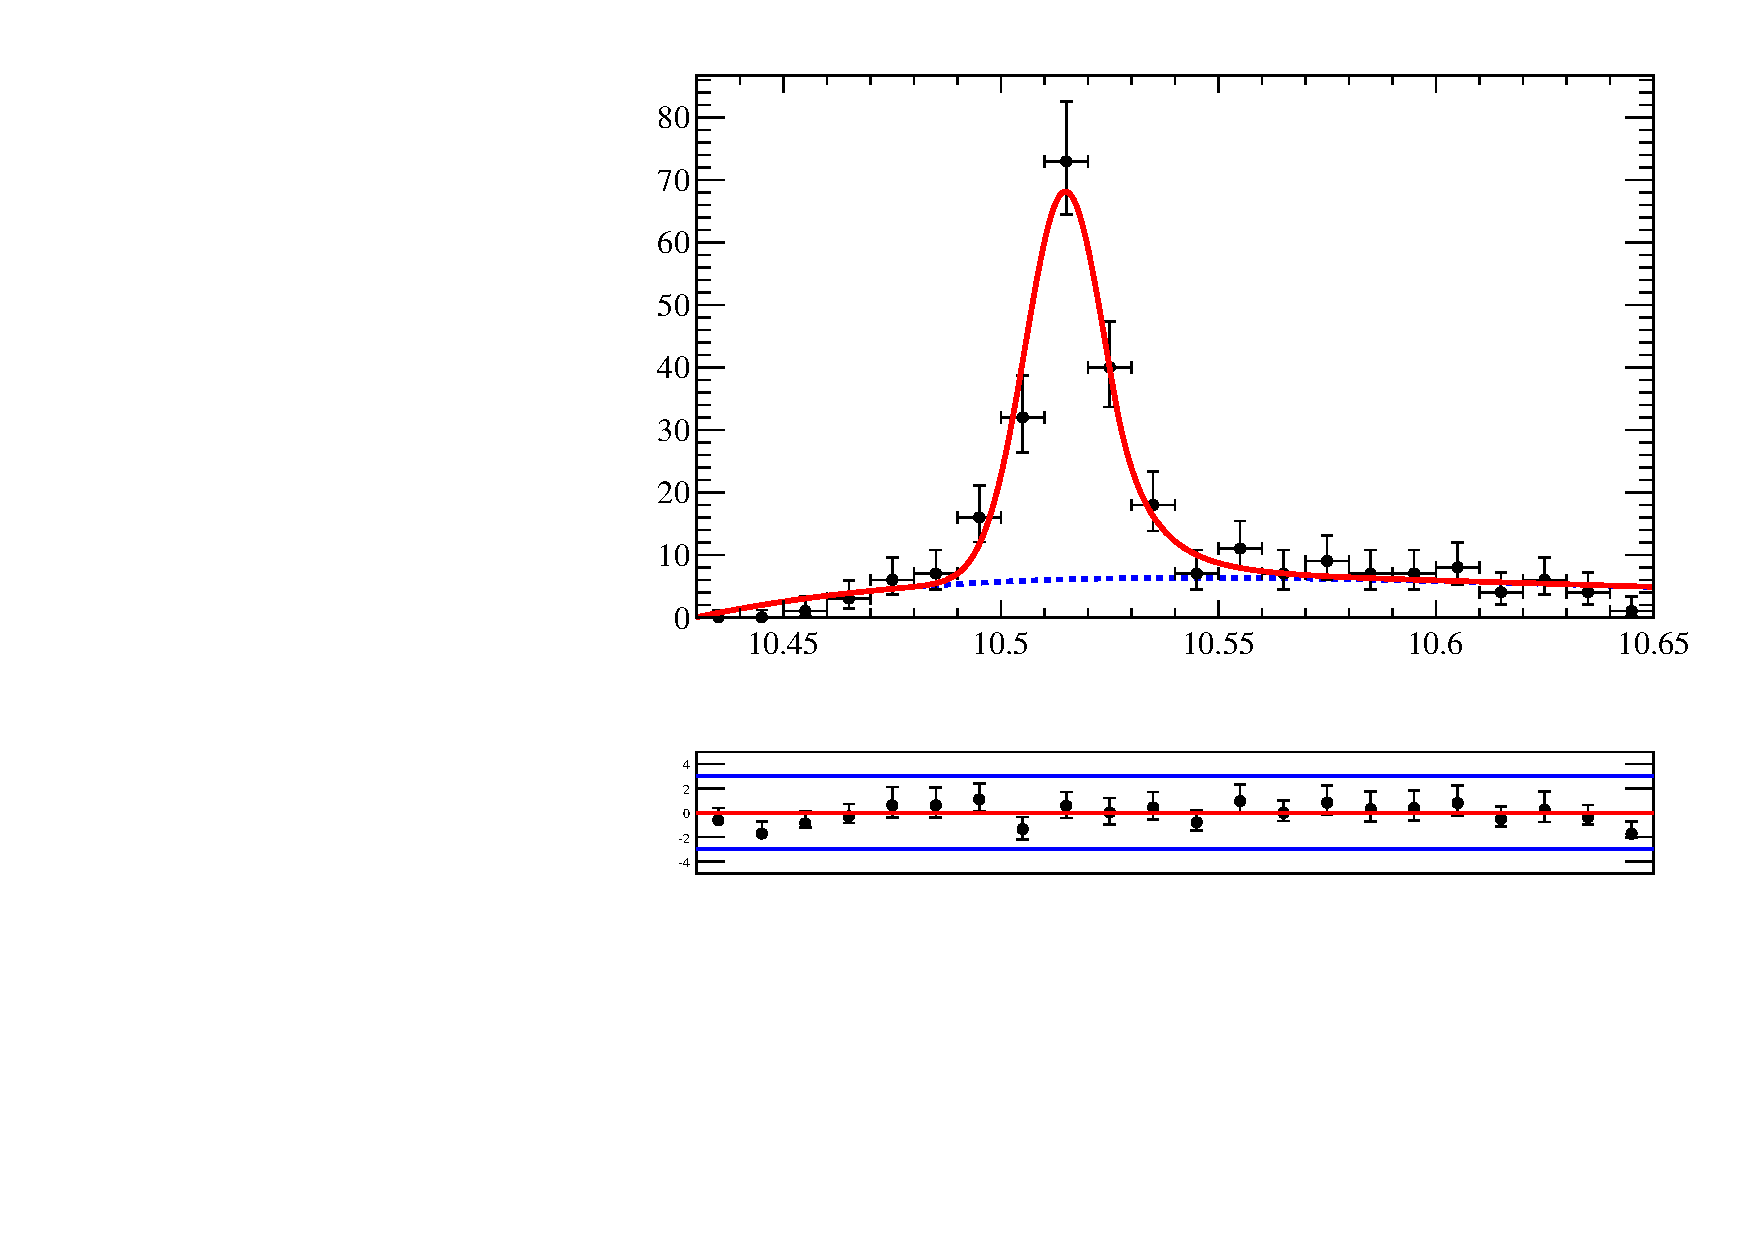
\includegraphics[width=75mm, height=60mm]{mc-fits-figs/cb13_27_40}
    }
    \put(192,54){\scriptsize $\chiboneThreeP \to \Y3S \gamma$}
    \put(192,49){\scriptsize $27 < p_T^{\Y3S} < 40 \gevc$}
    \put(160,13){$m_{\mumu \gamma} - m_{\mumu} + m_{\Y3S}^{PDG} \left[\gevcc\right]$}
    \put(153,25){\scriptsize \begin{sideways}Candidates/(10\mevcc)\end{sideways}}    
    % \put(195,43){\scriptsize N = 154 $\pm$ 17}
    % \put(195,40){\scriptsize B = 113 $\pm$ 16 (42 $\pm$ 7\%)}
    

     % \graphpaper[5](0,0)(225, 120)        
  \end{picture}
 }

\end{frame}
\begin{frame}{Data --- Monte Carlo comparison (1)}
A comparison of the distribution of the relevant observables used in this
analysis was performed on real and simulated data, in order to assess the
reliability of Monte Carlo in computing efficiencies

\begin{center}
\scalebox{0.38}{
  \setlength{\unitlength}{1mm}
  \begin{picture}(150,140)
    %
    \put(0,0){
      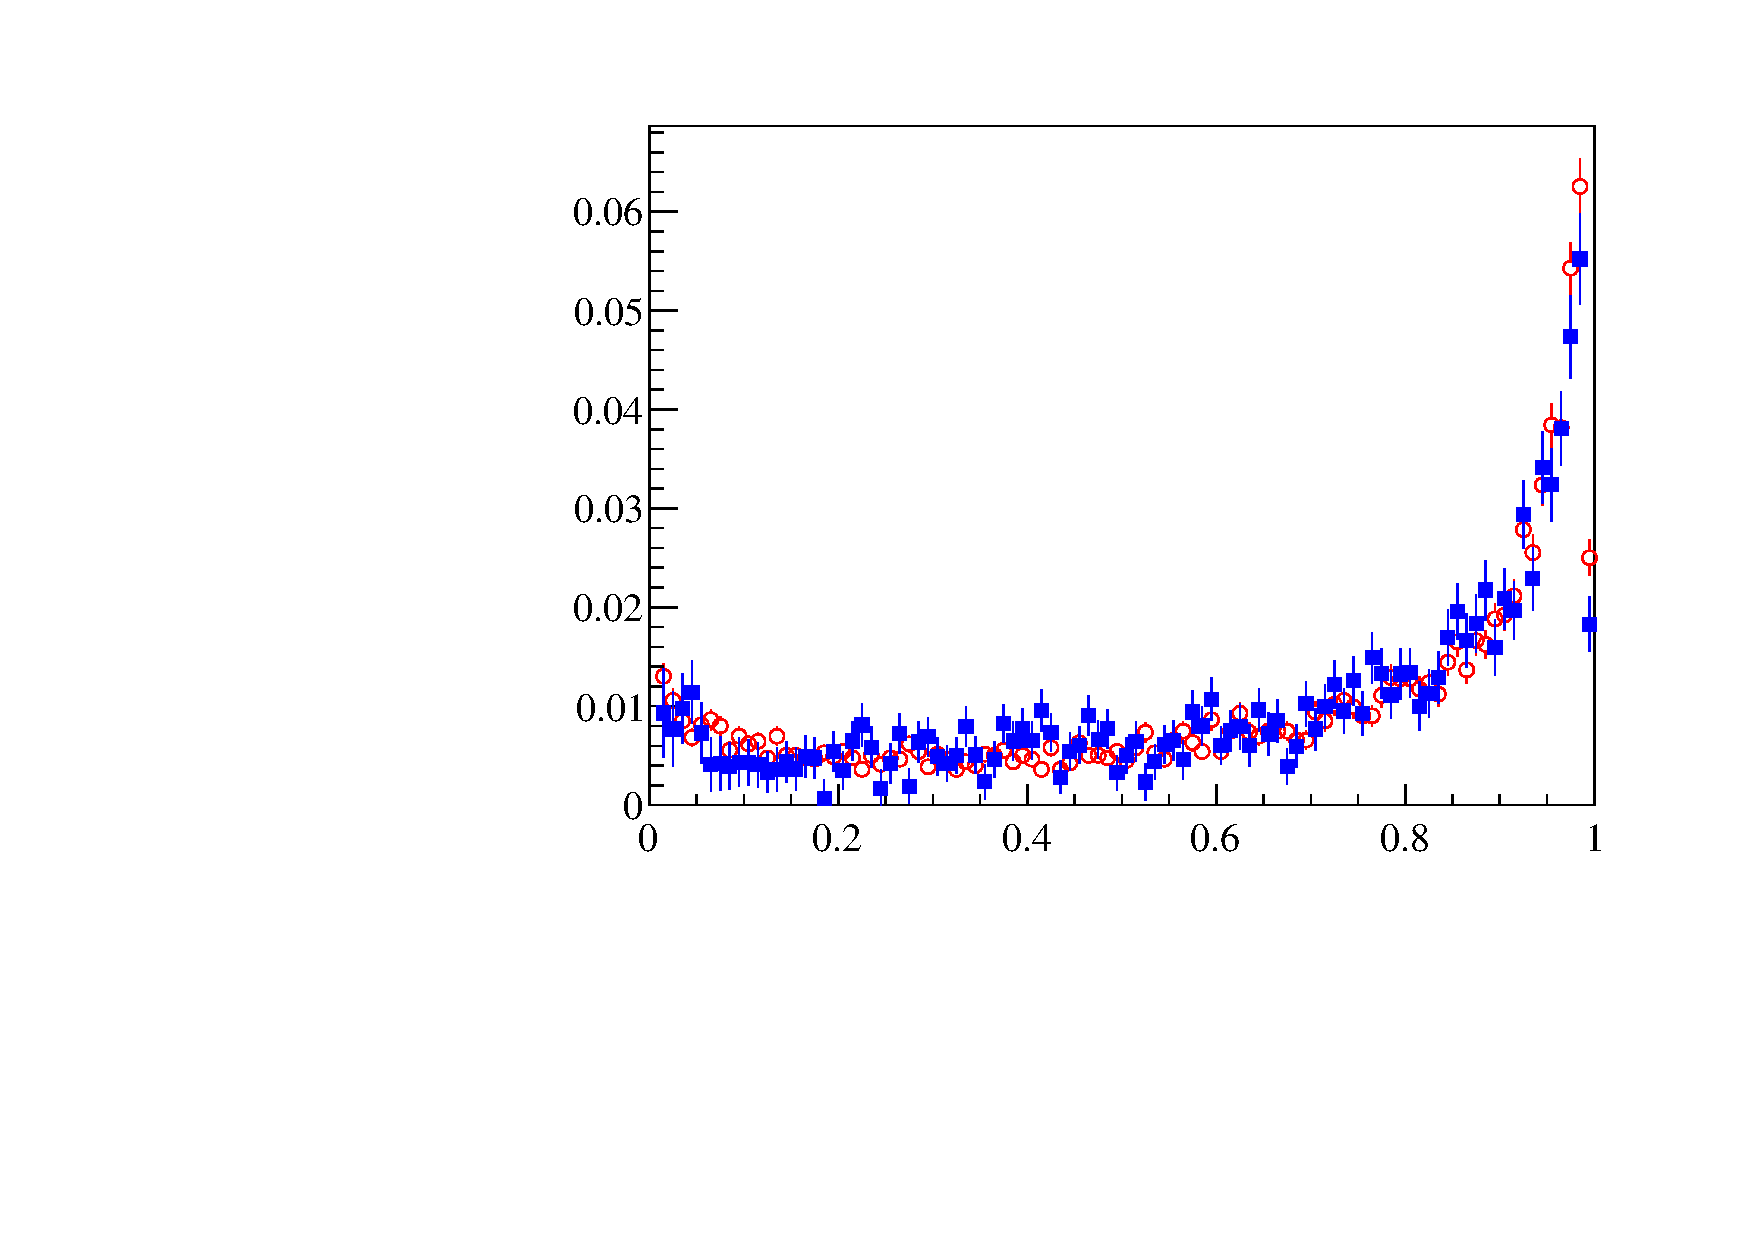
\includegraphics[width=50mm, height=35mm]{mc-data/cl_g_1p}
    }
    \put(50,0){
      \includegraphics[width=50mm, height=35mm]{mc-data/cl_g_2p}
    }
    \put(100,0){
      \includegraphics[width=50mm, height=35mm]{mc-data/cl_g_3p}
    }

    \put(0,35){
      \includegraphics[width=50mm, height=35mm]{mc-data/c2_dtf_1p}
    }
    \put(50,35){
      \includegraphics[width=50mm, height=35mm]{mc-data/c2_dtf_2p}
    }
    \put(100,35){
      \includegraphics[width=50mm, height=35mm]{mc-data/c2_dtf_3p}
    }
    \put(0,70){
      \includegraphics[width=50mm, height=35mm]{mc-data/pt_chib_1p}
    }
    \put(50,70){
      \includegraphics[width=50mm, height=35mm]{mc-data/pt_chib_2p}
    }
    \put(100,70){
      \includegraphics[width=50mm, height=35mm]{mc-data/pt_chib_3p}
    }
    \put(0,105){
      \includegraphics[width=50mm, height=35mm]{mc-data/pt_ups_1p}
    }
    \put(50,105){
      \includegraphics[width=50mm, height=35mm]{mc-data/pt_ups_2p}
    }
    \put(100,105){
      \includegraphics[width=50mm, height=35mm]{mc-data/pt_ups_3p}
    }

    \put(15,-1){\scriptsize $\gamma$ confidence level}
    \put(65,-1){\scriptsize $\gamma$ confidence level}
    \put(115,-1){\scriptsize $\gamma$ confidence level}
    \put(10,34){\scriptsize $\chisq$ of decay tree fitter}
    \put(60,34){\scriptsize $\chisq$ of decay tree fitter}
    \put(110,34){\scriptsize $\chisq$ of decay tree fitter}
    \put(20,69){\scriptsize $p_T[\chibOneP] \left[\gevcc\right]$}
    \put(70,69){\scriptsize $p_T[\chibTwoP] \left[\gevcc\right]$}
    \put(120,69){\scriptsize $p_T[\chibThreeP] \left[\gevcc\right]$}
    \put(20,104){\scriptsize $p_T[\Y1S] \left[\gevcc\right]$}
    \put(70,104){\scriptsize $p_T[\Y1S] \left[\gevcc\right]$}
    \put(120,104){\scriptsize $p_T[\Y1S] \left[\gevcc\right]$}

    \put(0,7){\scriptsize \begin{sideways}Arbitrary units\end{sideways}}
    \put(50,7){\scriptsize \begin{sideways}Arbitrary units\end{sideways}}
    \put(100,7){\scriptsize \begin{sideways}Arbitrary units\end{sideways}}
    \put(0,42){\scriptsize \begin{sideways}Arbitrary units\end{sideways}}
    \put(50,42){\scriptsize \begin{sideways}Arbitrary units\end{sideways}}
    \put(100,42){\scriptsize \begin{sideways}Arbitrary units\end{sideways}}
    \put(0,77){\scriptsize \begin{sideways}Arbitrary units\end{sideways}}
    \put(50,77){\scriptsize \begin{sideways}Arbitrary units\end{sideways}}
    \put(100,77){\scriptsize \begin{sideways}Arbitrary units\end{sideways}}
    \put(0,112){\scriptsize \begin{sideways}Arbitrary units\end{sideways}}
    \put(50,112){\scriptsize \begin{sideways}Arbitrary units\end{sideways}}
    \put(100,112){\scriptsize \begin{sideways}Arbitrary units\end{sideways}}

    \put(35,27){\scriptsize \chibOneP}
    \put(85,27){\scriptsize \chibTwoP}
    \put(135,27){\scriptsize \chibThreeP}
    \put(35,62){\scriptsize \chibOneP}
    \put(85,62){\scriptsize \chibTwoP}
    \put(135,62){\scriptsize \chibThreeP}
    \put(35,97){\scriptsize \chibOneP}
    \put(85,97){\scriptsize \chibTwoP}
    \put(135,97){\scriptsize \chibThreeP}
    \put(35,132){\scriptsize \chibOneP}
    \put(85,132){\scriptsize \chibTwoP}
    \put(135,132){\scriptsize \chibThreeP}
 
    % \graphpaper[5](0,0)(150, 175)        
  \end{picture}
}
\end{center}
\begin{block}{}
The agreement is generally very good.
\end{block}

\end{frame}

\begin{frame}{Data --- Monte Carlo comparison (2)}

\begin{center}
\resizebox{\textwidth}{!}{
  \setlength{\unitlength}{1mm}
  \begin{picture}(150,70)
    %
    \put(0,0){
      \includegraphics[width=50mm, height=35mm]{mc-data/pt_g_1p}
    }
    \put(50,0){
      \includegraphics[width=50mm, height=35mm]{mc-data/pt_g_2p}
    }
    \put(100,0){
      \includegraphics[width=50mm, height=35mm]{mc-data/pt_g_3p}
    }

    \put(15,-1){\scriptsize $p_T(\gamma) [\gevc]$ }
    \put(65,-1){\scriptsize $p_T(\gamma) [\gevc]$}
    \put(115,-1){\scriptsize $p_T(\gamma) [\gevc]$}

    \put(0,7){\scriptsize \begin{sideways}Arbitrary units\end{sideways}}
    \put(50,7){\scriptsize \begin{sideways}Arbitrary units\end{sideways}}
    \put(100,7){\scriptsize \begin{sideways}Arbitrary units\end{sideways}}

    \put(35,27){\scriptsize \chibOneP}
    \put(85,27){\scriptsize \chibTwoP}
    \put(135,27){\scriptsize \chibThreeP}
 
    % \graphpaper[5](0,0)(150, 175)        
  \end{picture}
}
\end{center}
\begin{alertblock}{}
This is due to the \sPlot\ technique, when applied on variables that affect the
background shape. In our study the background in the fit of the invariant mass
distribution depends on the photon transverse momentum, hence a mismatch
between data and simulation is expected.
\end{alertblock}

\end{frame}

\begin{frame}{Monte-Carlo photon reconstruction efficiency}
\begin{columns}
\column{.5\textwidth}
\setlength{\unitlength}{1mm}
\centering
\resizebox{.9\textwidth}{!}{
\begin{picture}(150,180)
\put(0,0){\includegraphics*[width=75mm,height=60mm]{mc-eff/ups2_3}}
\put(2,18){\begin{sideways}Efficiency, \%\end{sideways}}
\put(34,0){$p_T^{\Y2S} \left[\gevc\right]$}
\put(30,24){$\chi_b(3P) \to \Upsilon(2S) \gamma$}
\put(30,18){\includegraphics*[width=4mm, height=2mm]{blue}}
\put(35,18){\small \textcolor{blue}{\sqs=7\tev}}
\put(30,13){\includegraphics*[width=4mm, height=2mm]{red}}
\put(35,13){\small \textcolor{red}{\sqs=8\tev}}

\put(75,0){\includegraphics*[width=75mm,height=60mm]{mc-eff/ups3_3}}
\put(77,18){\begin{sideways}Efficiency, \%\end{sideways}}
\put(109,0){$p_T^{\Y3S} \left[\gevc\right]$}
\put(105,24){$\chi_b(3P) \to \Upsilon(3S) \gamma$}
\put(105,18){\includegraphics*[width=4mm, height=2mm]{blue}}
\put(110,18){\small \textcolor{blue}{\sqs=7\tev}}
\put(105,13){\includegraphics*[width=4mm, height=2mm]{red}}
\put(110,13){\small \textcolor{red}{\sqs=8\tev}}

\put(0,60){\includegraphics*[width=75mm,height=60mm]{mc-eff/ups1_3}}
\put(2,78){\begin{sideways}Efficiency, \%\end{sideways}}
\put(34,60){$p_T^{\Y1S} \left[\gevc\right]$}
\put(30,84){$\chi_b(3P) \to \Upsilon(1S) \gamma$}
\put(30,78){\includegraphics*[width=4mm, height=2mm]{blue}}
\put(35,78){\small \textcolor{blue}{\sqs=7\tev}}
\put(30,73){\includegraphics*[width=4mm, height=2mm]{red}}
\put(35,73){\small \textcolor{red}{\sqs=8\tev}}

\put(75,60){\includegraphics*[width=75mm,height=60mm]{mc-eff/ups2_2}}
\put(77,78){\begin{sideways}Efficiency, \%\end{sideways}}
\put(109,60){$p_T^{\Y2S} \left[\gevc\right]$}
\put(105,84){$\chi_b(2P) \to \Upsilon(2S) \gamma$}
\put(105,78){\includegraphics*[width=4mm, height=2mm]{blue}}
\put(110,78){\small \textcolor{blue}{\sqs=7\tev}}
\put(105,73){\includegraphics*[width=4mm, height=2mm]{red}}
\put(110,73){\small \textcolor{red}{\sqs=8\tev}}

\put(0,120){\includegraphics*[width=75mm,height=60mm]{mc-eff/ups1_1}}
\put(2,138){\begin{sideways}Efficiency, \%\end{sideways}}
\put(34,120){$p_T^{\Y1S} \left[\gevc\right]$}
\put(30,144){$\chi_b(1P) \to \Upsilon(1S) \gamma$}
\put(30,138){\includegraphics*[width=4mm, height=2mm]{blue}}
\put(35,138){\small \textcolor{blue}{\sqs=7\tev}}
\put(30,133){\includegraphics*[width=4mm, height=2mm]{red}}
\put(35,133){\small \textcolor{red}{\sqs=8\tev}}

\put(75,120){\includegraphics*[width=75mm,height=60mm]{mc-eff/ups1_2}}
\put(77,138){\begin{sideways}Efficiency, \%\end{sideways}}
\put(109,120){$p_T^{\Y1S} \left[\gevc\right]$}
\put(105,144){$\chi_b(2P) \to \Upsilon(1S) \gamma$}
\put(105,138){\includegraphics*[width=4mm, height=2mm]{blue}}
\put(110,138){\small \textcolor{blue}{\sqs=7\tev}}
\put(105,133){\includegraphics*[width=4mm, height=2mm]{red}}
\put(110,133){\small \textcolor{red}{\sqs=8\tev}}
  
  % \graphpaper[5](0,0)(75, 60)
\end{picture}
} % end scalebox
\column{.5\textwidth}
Photon is more energetic as $p_T(\Upsilon)$ increases so it is reconstructed more efficiently.
\end{columns}
\end{frame}
\begin{frame}{Systematic uncertainties}
Since this analysis measures the fraction of $\Upsilon(nS)$ particles
originating from $\chi_b$ decays, most systematic uncertainties cancel in the
ratio and only residual effects need to be taken into account. 

\bigskip

Systematic uncertainties on the event yields are mostly
due to the fit model of $\Upsilon$ and $\chi_b$ invariant masses, while the
ones on the efficiency are due to the photon reconstruction and the unknown
initial polarization of $\chi_b$ and $\Upsilon$ particles.
\end{frame}
\begin{frame}{$\chi_b$ yields systematic uncertainties. Unknown $\sigma{\chi_{b2}}/\sigma{\chi_{b1}}$ ratio (1)}

\centering

The $\sigma(\chi_{b2})/\sigma(\chi_{b1})$ ratio prediction:

\resizebox{.5\textwidth}{!}{
\setlength{\unitlength}{1mm}
\begin{picture}(75,60)
%
 \put(0,0){\includegraphics[width=75mm, height=60mm]{theory/ratio}}
 \put(-1,22){\begin{sideways}$\sigma({\chi_2})/\sigma({\chi_1}$)\end{sideways}}
\end{picture}
} 

\footnotesize
Transverse momentum distributions of the
$d\sigma\left[\chi_{2}\right]/d\sigma[\chi_{1}]$ ratio. Solid and dashed lines
stand for charmonium and bottomonium mesons. The dot-dashed line corresponds to
the rescaled bottomonium ratio:
$\sigma_{b2}/\sigma_{b1}(M_{\chi_c}/M_{\chi_b}p_T)$. The experimental results
for charmonium from LHCb are shown with dots, CDF --- with rectangles, and CMS
--- with triangles.
\end{frame}

\begin{frame}{$\chi_b$ yields systematic uncertainties. Unknown $\sigma{\chi_{b2}}/\sigma{\chi_{b1}}$ ratio (2)}
\definecolor{LRed}{rgb}{1,.8,.8}
{\footnotesize $\chi_b$ yields systematic uncertainties (\%)  related to
unknown $\lambda=N_{\chi_{b1}}/(N_{\chi_{b1}}+N_{\chi_{b2}})$  ratio in the fit
model for  $\chi_b(1,2,3P) \to \OneS \gamma$ decays.\\
Systematic uncertanties are
measured in each $p_T^{\Upsilon}$ bin and center-of-mass energy. }

\bigskip

\centering

\resizebox{.5\textwidth}{!}{
\begin{tabular}{lrrrrrrrrrrrr}\toprule
 & \multicolumn{12}{c}{$\Upsilon(1S)$ transverse momentum intervals, \gevc}\\
 & \multicolumn{6}{c}{6 -- 8} & \multicolumn{6}{c}{8 -- 10}\\
\cmidrule(r){2-7}\cmidrule(r){8-13}
 & \multicolumn{3}{c}{\sqs = 7\tev} & \multicolumn{3}{c}{\sqs = 8\tev} & \multicolumn{3}{c}{\sqs = 7\tev} & \multicolumn{3}{c}{\sqs = 8\tev}\\
\cmidrule(r){2-4}\cmidrule(r){5-7}\cmidrule(r){8-10}\cmidrule(r){11-13}
 & \multicolumn{1}{c}{$N_{\chi_{b}(1P)}$} & \multicolumn{1}{c}{$N_{\chi_{b}(2P)}$} & \multicolumn{1}{c}{$N_{\chi_{b}(3P)}$} & \multicolumn{1}{c}{$N_{\chi_{b}(1P)}$} & \multicolumn{1}{c}{$N_{\chi_{b}(2P)}$} & \multicolumn{1}{c}{$N_{\chi_{b}(3P)}$} & \multicolumn{1}{c}{$N_{\chi_{b}(1P)}$} & \multicolumn{1}{c}{$N_{\chi_{b}(2P)}$} & \multicolumn{1}{c}{$N_{\chi_{b}(3P)}$} & \multicolumn{1}{c}{$N_{\chi_{b}(1P)}$} & \multicolumn{1}{c}{$N_{\chi_{b}(2P)}$} & \multicolumn{1}{c}{$N_{\chi_{b}(3P)}$}\\
\midrule
$\lambda=0.0$ & 13.3 & -8.3 & --- & 10.1 & -12.9 & --- & 19.3 & -8.7 & --- & 15.9 & -7.3 & ---\\
$\lambda=0.1$ & 9.0 & -6.7 & --- & 6.1 & -8.9 & --- & 13.9 & -7.0 & --- & 11.1 & -5.9 & ---\\
$\lambda=0.2$ & 5.4 & -5.2 & --- & 2.9 & -5.4 & --- & 9.1 & -5.2 & --- & 6.9 & -4.2 & ---\\

\rule{0pt}{4ex}$\lambda=0.3$ & 2.5 & -3.4 & --- & 0.8 & -3.9 & --- & 4.9 & -3.2 & --- & 3.6 & -2.6 & ---\\
\rowcolor{LRed}$\lambda=0.4$ & 0.7 & -1.6 & --- & -0.3 & -1.5 & --- & 1.9 & -1.5 & --- & 1.2 & -1.1 & ---\\
\rowcolor{LRed}$\lambda=0.5$ & 0.0 & 0.0 & --- & 0.0 & 0.0 & --- & 0.0 & 0.0 & --- & 0.0 & 0.0 & ---\\
\rowcolor{LRed}$\lambda=0.6$ & 0.8 & 1.5 & --- & 1.3 & 0.7 & --- & -0.7 & 1.2 & --- & 0.1 & 0.8 & ---\\
\rowcolor{LRed}$\lambda=0.7$ & 2.7 & 1.6 & --- & 4.1 & -2.2 & --- & -0.1 & 1.9 & --- & 1.4 & 1.0 & ---\\

\rule{0pt}{4ex}$\lambda=0.8$ & 6.1 & 0.8 & --- & 7.1 & -8.3 & --- & 1.6 & 2.2 & --- & 3.7 & 0.9 & ---\\
$\lambda=0.9$ & 9.4 & -1.3 & --- & 10.9 & -17.2 & --- & 4.3 & 2.0 & --- & 7.1 & 0.5 & ---\\
$\lambda=1.0$ & 13.9 & -5.8 & --- & 14.7 & -24.4 & --- & 7.9 & 1.7 & --- & 11.2 & -0.4 & ---\\
\bottomrule
\end{tabular}
}

\resizebox{.5\textwidth}{!}{
\begin{tabular}{lrrrrrrrrrrrr}\toprule
 & \multicolumn{12}{c}{$\Upsilon(1S)$ transverse momentum intervals, \gevc}\\
 & \multicolumn{6}{c}{10 -- 14} & \multicolumn{6}{c}{14 -- 18}\\
\cmidrule(r){2-7}\cmidrule(r){8-13}
 & \multicolumn{3}{c}{\sqs = 7\tev} & \multicolumn{3}{c}{\sqs = 8\tev} & \multicolumn{3}{c}{\sqs = 7\tev} & \multicolumn{3}{c}{\sqs = 8\tev}\\
\cmidrule(r){2-4}\cmidrule(r){5-7}\cmidrule(r){8-10}\cmidrule(r){11-13}
 & \multicolumn{1}{c}{$N_{\chi_{b}(1P)}$} & \multicolumn{1}{c}{$N_{\chi_{b}(2P)}$} & \multicolumn{1}{c}{$N_{\chi_{b}(3P)}$} & \multicolumn{1}{c}{$N_{\chi_{b}(1P)}$} & \multicolumn{1}{c}{$N_{\chi_{b}(2P)}$} & \multicolumn{1}{c}{$N_{\chi_{b}(3P)}$} & \multicolumn{1}{c}{$N_{\chi_{b}(1P)}$} & \multicolumn{1}{c}{$N_{\chi_{b}(2P)}$} & \multicolumn{1}{c}{$N_{\chi_{b}(3P)}$} & \multicolumn{1}{c}{$N_{\chi_{b}(1P)}$} & \multicolumn{1}{c}{$N_{\chi_{b}(2P)}$} & \multicolumn{1}{c}{$N_{\chi_{b}(3P)}$}\\
\midrule
$\lambda=0.0$ & 15.8 & -3.1 & 36.1 & 13.7 & -13.6 & 36.2 & 6.8 & -0.9 & 5.3 & 7.3 & -2.0 & -9.5\\
$\lambda=0.1$ & 10.7 & -2.6 & 25.9 & 5.5 & -7.0 & -0.6 & 4.2 & -1.0 & 5.5 & 4.7 & -1.9 & -5.7\\
$\lambda=0.2$ & 6.3 & -1.7 & 16.6 & 5.2 & -6.3 & 16.8 & 2.2 & -1.0 & 5.1 & 2.5 & -1.6 & -3.1\\

\rule{0pt}{4ex}$\lambda=0.3$ & 3.0 & -0.9 & 9.0 & 2.6 & -3.4 & 9.3 & 0.9 & -0.9 & 3.9 & 1.1 & -1.2 & -1.2\\
\rowcolor{LRed}$\lambda=0.4$ & 0.9 & -0.2 & 3.6 & 0.2 & -0.9 & 0.9 & 0.1 & -0.5 & 2.1 & 0.2 & -0.6 & -0.0\\
\rowcolor{LRed}$\lambda=0.5$ & 0.0 & 0.0 & 0.0 & 0.0 & 0.0 & 0.0 & 0.0 & 0.0 & 0.0 & 0.0 & 0.0 & 0.0\\
\rowcolor{LRed}$\lambda=0.6$ & 0.4 & -0.2 & -2.1 & 0.6 & 0.6 & -1.5 & 0.7 & 0.3 & -6.2 & 0.5 & 0.9 & -0.7\\
\rowcolor{LRed}$\lambda=0.7$ & 1.9 & -1.0 & -2.9 & 2.5 & 0.3 & 1.4 & 1.6 & 2.2 & -4.8 & 1.6 & 2.0 & -1.8\\

\rule{0pt}{4ex}$\lambda=0.8$ & 4.4 & -2.0 & -3.0 & 4.1 & -0.2 & -4.8 & 3.1 & 4.4 & -3.5 & 3.2 & 3.4 & -3.4\\
$\lambda=0.9$ & 7.8 & -3.3 & -1.8 & 9.0 & -1.6 & 7.5 & 5.4 & 5.7 & -9.6 & 5.5 & 5.2 & -4.7\\
$\lambda=1.0$ & 12.0 & -4.8 & 0.4 & 13.3 & -3.1 & 9.4 & 8.1 & 8.1 & -11.4 & 8.3 & 7.3 & -5.9\\
\bottomrule
\end{tabular}

}

\begin{block}{}
\centering
Theory predicts that $\lambda$ belongs to the range between 0.4 and 0.7. 
\end{block}

\end{frame}
\begin{frame}{Systematic uncertainties due to $\chib$ polarization}
\begin{block}{}
\small
Efficiencies are evaluated on MC where \chib particles are unpolarized. To evaluate systematic effects due to the unknown polarization of \chib, MC events are reweighted as described in \textcolor{blue}{HERA-B Collaboration, I. Abt et al.,  Production of the Charmonium States $\chi_{c1}$ and $\chi_{c2}$ in Proton Nucleus Interactions at s = 41.6-GeV}, \href{http://arxiv.org/abs/0807.2167}{arXiv:0807.2167} and
\textcolor{blue}{LHCb collaboration, R. Aaij et al.,Measurement of the cross-section ratio $\sigma(\chi_{c2})/\sigma(\chi_{c1})$ for prompt $\chi_c$
production at $\sqrt{s}=7$ TeV}, \href{http://arxiv.org/abs/1202.1080}{arXiv:1202.1080}
\end{block}
For each simulated event in the unpolarised sample, a weight is calculated from
the distribution of the following angles in the various polarisation hypotheses compared to the
unpolarised distribution.

\scalebox{0.7}{
\begin{tabular}{c|p{10cm}}\toprule
$\Theta_{\Upsilon}$ & angle between the directions of the $\mu^{+}$ in the $\Upsilon$ rest frame and the $\Upsilon$ in the $\chi_b$ rest frame.\\
\midrule
$\Theta_{\chi_b}$ & angle between the directions of the $\Upsilon$ in the $\chi_b$ rest frame and $\chi_b$ in the lab frame.\\
\midrule
$\phi$ & angle between the $\Upsilon$ decay plane in the $\chi_b$ rest frame and the plane formed by $\chi_b$ direction in the lab frame and the direction of the $\Upsilon$ in the $\chi_b$ rest frame.\\
\bottomrule
\end{tabular}
}

\vspace{0.1in}

Two hypotheses for $\chibone$ state (w0, w1) and three hypotheses for $\chibtwo$ (w0, w1, w2).

\end{frame}
\begin{frame}{Systematic uncertainties due to \chib polarization}
The ratio of efficiency for unpolarized \chib to efficiency for polarized \chib.

\resizebox{\textwidth}{!}{
\setlength{\unitlength}{1mm}
  \begin{picture}(150,60)
    \put(0,0){
      \includegraphics*[width=75mm, height=45mm]{polarization/chib11p_ups1s_w0_ratio}
    }
    \put(75,0){
      \includegraphics*[width=75mm, height=45mm]{polarization/chib11p_ups1s_w1_ratio}
    }

    \put(50,0){$p_T^{\Y1S} \left[\gevc\right]$}
    \put(125,0){$p_T^{\Y1S} \left[\gevc\right]$}

    \put(50,0){$p_T^{\Y1S} \left[\gevc\right]$}
    \put(125,0){$p_T^{\Y1S} \left[\gevc\right]$}


    \put(0,20){\begin{sideways}$\eps_{m_{\chi_{b1}}} / \eps_{unpol}$\end{sideways}}
    \put(75,20){\begin{sideways}$\eps_{m_{\chi_{b1}}} / \eps_{unpol}$\end{sideways}}
 
    \put(40,36){\small $\chiboneOneP \to \Y1S \gamma$}
    \put(40,30){\small $|m_{\chi_{b1}}|=0$}
    \put(110,20){\small $\chiboneOneP \to \Y1S \gamma$}
    \put(110,14){\small $|m_{\chi_{b1}}|=1$}
 
  \end{picture}
}

\begin{block}{}
The difference between ratio and 1 is considered as systematic uncertainty.
\end{block}

\end{frame}
\begin{frame}{Summary of systematic uncertainties}
\begin{center}
$\Upsilon$ fraction uncertainties common to all \chib decays (\%)
% \scale{.75\textwidth}{!}{
\begin{tabular}{lc}
\toprule
$\Upsilon$ fit model & $\pm 0.7$ \\
$\gamma$ reconstruction & $\pm 3$ \\
\bottomrule
\end{tabular}
% }
\bigskip

Summary of $\Upsilon$ fraction systematic uncertainties (\%)\\
(maximum deviations that were found in $p_T^{\Upsilon}$ bins):

\scalebox{.75}{
\begin{tabular}{lcc}
\toprule
&  \chib fit model & \chib polarization\\
\midrule
\rule{0pt}{4ex}$\chib(1P) \to \Y1S \gamma$ & ${}^{+4.3}_{-5.8}$ & ${}^{+5.1}_{-4.0}$\\
\rule{0pt}{4ex}$\chib(2P) \to \Y1S \gamma$ & ${}^{+4.8}_{-6.2}$ & ${}^{+5.8}_{-6.8}$\\
\rule{0pt}{4ex}$\chib(3P) \to \Y1S \gamma$ & ${}^{+19.6}_{-16.6}$ & ${}^{+6.9}_{-6.7}$\\
\rule{0pt}{4ex}$\chib(2P) \to \Y2S \gamma$ & ${}^{+2.3}_{-7.0}$ & ${}^{+8.7}_{-7.8}$\\
\rule{0pt}{4ex}$\chib(3P) \to \Y2S \gamma$ & ${}^{+19.7}_{-19.9}$ & ${}^{+4.5}_{-4.2}$\\
\rule{0pt}{4ex}$\chib(3P) \to \Y3S \gamma$ & ${}^{+20.9}_{-27.6}$ & ${}^{+6.4}_{-7.5}$\\
\bottomrule
\end{tabular}
}
\end{center}
\end{frame}
\begin{frame}{$\Upsilon$ fractions in $\chib \to \Upsilon \gamma$ decays}
\setlength{\unitlength}{1mm}
\begin{columns}
\column{.5\textwidth}
  \resizebox{!}{.8\textheight}{
  \begin{picture}(150,180)
    %% =======================================================================
    \put(0,120){
      \includegraphics*[width=75mm, height=60mm]{results/ups1s_1}
    }
    \put(2,145){\begin{sideways}\Y1S fraction, \% \end{sideways}}
    \put(35,122){$p_T^{\Y1S} \left[\gevc\right]$}

    \put(15,173){\scriptsize $\chibOneP \to \Y1S \gamma$}
    
    \put(20,169){\scriptsize \textcolor{blue}{\sqs=7\tev}}
    \put(20,165){\scriptsize \textcolor{red}{\sqs=8\tev}}
    % \put(48,140){\scriptsize \textcolor{cyan}{\sqs=7\tev (2010)}}
    
    \put(15,169){\includegraphics*[width=4mm, height=2mm]{blue}}
    \put(15,165){\includegraphics*[width=4mm, height=2mm]{red}}
    % \put(43,140){\includegraphics*[width=4mm, height=2mm]{cyan}}
    %% =======================================================================
    \put(75,120){
      \includegraphics*[width=75mm, height=60mm]{results/ups1s_2}
    }
    \put(77,145){\begin{sideways}\Y1S fraction, \% \end{sideways}}
    \put(110,122){$p_T^{\Y1S} \left[\gevc\right]$}

    \put(90,173){\scriptsize $\chibTwoP \to \Y1S \gamma$}
    
    \put(95,169){\scriptsize \textcolor{blue}{\sqs=7\tev}}
    \put(95,165){\scriptsize \textcolor{red}{\sqs=8\tev}}
    
    
    \put(90,169){\includegraphics*[width=4mm, height=2mm]{blue}}
    \put(90,165){\includegraphics*[width=4mm, height=2mm]{red}}
    
    %% =======================================================================
    \put(0,60){
      \includegraphics*[width=75mm, height=60mm]{results/ups1s_3}
    }
    \put(2,85){\begin{sideways}\Y1S fraction, \% \end{sideways}}
    \put(35,62){$p_T^{\Y1S} \left[\gevc\right]$}

    \put(15,113){\scriptsize $\chibThreeP \to \Y1S \gamma$}
    \put(20,108){\scriptsize \textcolor{blue}{\sqs=7\tev}}
    \put(20,104){\scriptsize \textcolor{red}{\sqs=8\tev}}
    
    
    \put(15,108){\includegraphics*[width=4mm, height=2mm]{blue}}
    \put(15,104){\includegraphics*[width=4mm, height=2mm]{red}}
    
    %% =======================================================================
    \put(75,60){
      \includegraphics*[width=75mm, height=60mm]{results/ups2s_2}
    }
    \put(77,85){\begin{sideways}\Y2S fraction, \% \end{sideways}}
    \put(110,62){$p_T^{\Y2S} \left[\gevc\right]$}

    \put(90,113){\scriptsize $\chibTwoP \to \Y2S \gamma$}
    \put(95,109){\scriptsize \textcolor{blue}{\sqs=7\tev}}
    \put(95,105){\scriptsize \textcolor{red}{\sqs=8\tev}}
    
    
    \put(90,109){\includegraphics*[width=4mm, height=2mm]{blue}}
    \put(90,105){\includegraphics*[width=4mm, height=2mm]{red}}
    
    %% =======================================================================
    \put(0,0){
      \includegraphics*[width=75mm, height=60mm]{results/ups2s_3}
    }
    \put(2,25){\begin{sideways}\Y2S fraction, \% \end{sideways}}
    \put(35,2){$p_T^{\Y2S} \left[\gevc\right]$}

    \put(15,53){\scriptsize $\chibThreeP \to \Y2S \gamma$}
    \put(20,48){\scriptsize \textcolor{blue}{\sqs=7\tev}}
    \put(20,44){\scriptsize \textcolor{red}{\sqs=8\tev}}
    
    
    \put(15,48){\includegraphics*[width=4mm, height=2mm]{blue}}
    \put(15,44){\includegraphics*[width=4mm, height=2mm]{red}}

    %% =======================================================================
    \put(75,0){
      \includegraphics*[width=75mm, height=60mm]{results/ups3s_3}
    }
    \put(77,25){\begin{sideways}\Y3S fraction, \% \end{sideways}}
    \put(110,2){$p_T^{\Y3S} \left[\gevc\right]$}

    \put(90,53){\scriptsize $\chibThreeP \to \Y3S \gamma$}
    \put(95,48){\scriptsize \textcolor{blue}{\sqs=7\tev}}
    \put(95,44){\scriptsize \textcolor{red}{\sqs=8\tev}}
    
    
    \put(90,48){\includegraphics*[width=4mm, height=2mm]{blue}}
    \put(90,44){\includegraphics*[width=4mm, height=2mm]{red}}
    
  % \graphpaper[5](0,0)(150, 180)
  \end{picture}
}
\column{.5\textwidth}
\resizebox{\textwidth}{!}{
\begin{picture}(80,60)
    %% =======================================================================
    \put(0,0){
      \includegraphics*[width=75mm, height=60mm]{results/ups1s_1_old}
    }
    \put(2,15){\begin{sideways}\Y1S fraction, \% \end{sideways}}
    \put(40,0){$p_T^{\Y1S} \left[\gevc\right]$}

    \put(40,30){\scriptsize $\chibOneP \to \Y1S \gamma$}
    
    \put(45,26){\scriptsize \textcolor{blue}{\sqs=7\tev}}
    \put(45,22){\scriptsize \textcolor{red}{\sqs=8\tev}}
    \put(45,18){\scriptsize \sqs=7\tev (2010)}
    
    \put(40,26){\includegraphics*[width=4mm, height=2mm]{blue}}
    \put(40,22){\includegraphics*[width=4mm, height=2mm]{red}}
    \put(40,18){\includegraphics*[width=4mm, height=2mm]{black}}

    
  % \graphpaper[5](0,0)(80, 60)
  \end{picture}
}

\bigskip

{\scriptsize
Outer error bars show statistical and systematics errors,
inner error bars --- only statistical errors.
}

\end{columns}
\end{frame}
\begin{frame}{Summary}

\begin{itemize}
\item Measured fractions of \Y1,2,3S originated from \chib decays.
About 40\% of $\Upsilon$ come from $\chi_b$, with mild dependence on $\Upsilon$ transverse momentum.
\item This analysis improves significantly the statistical precision of the previous work and 
adds more decays and transverse momentum regions.
% \item  The \lhcb detector design allows to perform measurements in $\Upsilon$ rapidity and 
% transverse momentum regions, which are complementary to the ones exploited 
% by \atlas and \cms.
\item Measured mass of $\chi_b(3P)$ is $10{,508}\pm2\stat\pm8\stat\mevcc$, consistent with another determination which uses converted photons.
\end{itemize}

% \begin{block}{}
% The results on \chib production were regularly presented at the LHCb bottomonium working group,
% an internal document was prepared by the author, is currently under review and will form 
% the basis of a future LHCb publication.
% \end{block}

\end{frame}
% \begin{frame}
\begin{exampleblock}{}
    \begin{center}
        {\huge High Level Trigger software performance profiling}
    \end{center}
\end{exampleblock}
\end{frame}

% \begin{frame}
Optimizing the LHCb trigger is crucial in many measurement. In particular,
decays with muons can be triggered on with \textbf{unprecedented high efficiency} ($\sim$80\%).
\begin{columns}[c]
\column{.5\textwidth}
\includegraphics[width=\textwidth]{profiler/mumu.png}
\column{.5\textwidth}
The dimuon trigger:

\begin{itemize}
  \item is not prescaled.
  \item is used in more than 50\% of LHCb's papers.
\end{itemize}
\end{columns}
\end{frame}
% \begin{frame}{Trigger software profiling}
\begin{columns}[c]
\column{.4\textwidth}
\includegraphics[width=.9\textwidth]{profiler/hlt_struct1.png}\\~\\
\textcolor{red}{The trigger needs fast algorithms!}
\column{.6\textwidth}
Most experiments require a trigger in order to record interesting events at suitable rate.
\begin{itemize}
  \item L0 Hardware Trigger $40 MHz \rightarrow 1 MHz$. Search for high pt, $\mu$, e, $\gamma$, hadron candidates.
  \item High Level Software Trigger Farm
  \begin{itemize}
    \item HLT1: Add Impact parameter cuts
    \item HLT2: Global event reconstruction.
  \end{itemize}
\end{itemize}
\begin{itemize}
  \item 100 man/years work that has only 20-30 ms to process an average event.
  \item 29K CPUs or 1700 servers.
  \item $2 \times 10^{15}$ bytes stored in 2012.
\end{itemize}
% \includegraphics[width=.8\textwidth]{images/moore.png}
\end{columns}
\end{frame}

% \begin{frame}
\frametitle{CPU Profiler Auditor}
CPU profiler tool is vital for trigger optimization.\\~\\
\begin{columns}[c]
\column{.5\textwidth}
\includegraphics[width=\textwidth]{profiler/cpu01.png}\\~\\
\includegraphics[width=\textwidth]{profiler/cpu02.png}
\column{.5\textwidth}
\begin{itemize}
    \item C++ library.
    \item Deployed into the core software framework in LHCb --- Gaudi.
    \item Based on Intel\textsuperscript{\textregistered} VTune\texttrademark
    Amplifier XE User API
    \item Full and clear reports.
\end{itemize}
\end{columns}
\end{frame}
% \begin{frame}{CHEP2012: Talk and Paper}
This work was presented on ``Computing in High Energy and Nuclear Physics'' conference.
The largest of the conferenes in this area. The conference is held every 18 months.
\begin{columns}[l]
\column{.4\textwidth}
\includegraphics[height=.6\textheight]{profiler/chep.png}
\column{.6\textwidth}
\begin{itemize}
    \item A. Mazurov and B. Couturier, ``Advanced modular software performance monitoring'',
    Journal of Physics: Conference Series 396 (2012), no. 5052054.
\end{itemize}
\end{columns}
\end{frame}

\begin{frame}
\begin{center}
    {\huge Thank you!}
\end{center}
\end{frame}

\end{document}
